\documentclass[]{article}
\usepackage{assignment}
\usepackage{amsmath}
\usepackage{codex}
\usepackage{listings}
\usepackage{xcolor}
\usepackage{titlesec}
\titleformat{\section}
  {\Large\scshape}{Session \thesection}{1em}{}
\title{H0E76A: Model Predictive Control\\\large--- Homework assignments ---}
%%%%%%%%%%%%%%%%%%%%%%%%%%%
\author{Andrea Alboni - r1030437} 
%%%%%%%%%%%%%%%%%%%%%%%%%%%

\newcommand{\acyear}{2024-2025}
\newcommand{\assignmentweight}{7/20}

\newcommand{\toledo}{Toledo}

\begin{document}
\maketitle



The assignments below are homework assignments related to the exercise sessions that are organized throughout the 
semester.
The assignments count for \assignmentweight{} of the total marks on this course, and are graded based on the following deliverables
\begin{deliverables}
\begin{itemize}
	\item A report containing the answers to the questions and any numerical values or plots that are asked in the assignments. 
	You can write your solutions directly in this \texttt{tex}-file. Make sure to fill in your name above. 
	\item A single zip-archive containing all the code to generate the plots included in your report. 
	Make sure to add a readme file describing which script(s) to run (and the working directory from which to do so) to reproduce your results.
	It is recommended that you have at least one separate script per session.
\end{itemize}
\end{deliverables}
Most of the assignments build upon the solutions obtained from the sessions.
Solutions for the exercise sessions will be made available on \toledo{} shortly after each session. 
Before submitting your final report, make sure that you verify your solutions from the sessions if you reuse them here. 

\section{LQR and Dynamic programming}
\begin{assignment} Compare the finite horizon controllers $K_{N}$ you computed during the session with the infinite horizon LQR controller.
\begin{itemize} 
	\item Implement the infinite horizon LQR controller $u = K_{\infty} x$ (with initial state $x_0 = (10,10)$).\footnote{Use \texttt{solve\_discrete\_are} from \texttt{scipy.linalg}.} Write the obtained value for $K_\infty$.
	\textbf{Remark.} Report your answers with at least four decimal places.
	\item Plot the simulated closed-loop trajectory of this controller with the trajectories of the finite-horizon controller. What happens as 
	you increase $N$?
	\item Explain this observation based on the recursion relation used earlier and 
	the discrete-time algebraic Riccati equation (DARE).
\end{itemize}
\end{assignment}

\begin{flushleft}
	The goal of this analysis is to compare the performance of finite-horizon controllers $K_N$, computed for various prediction horizons 
	$N$, with the infinite-horizon Linear Quadratic Regulator (LQR) controller $K_{\infty}$. The infinite-horizon controller is obtained by solving the 
	Discrete Algebraic Riccati Equation (DARE), which provides the optimal feedback gain $K_{\infty}$ for minimizing the infinite-horizon quadratic cost.
\end{flushleft}
\begin{itemize}
	\item The obtained value of $K_{\infty}$ is:
	\begin{lstlisting}[style=python]
		Kinf:  [[1.28645 2.31256]]
	\end{lstlisting}

	\item 	The analysis demonstrates, and the plots in figure \ref{fig:2x2grid} confirm, that increasing the prediction horizon $N$ improves the performance of the finite-horizon MPC. For small $N$, the controller struggles to approximate the long-term cost-to-go, leading to poor decision-making and significant deviation from the infinite-horizon LQR solution. 
	However, as $N$ increases, the finite-horizon MPC gradually captures more of the system's future behavior, reducing the mismatch between its terminal cost approximation and the true cost-to-go function. 
	Ultimately, for sufficiently large $N$, the finite-horizon MPC converges to the infinite-horizon LQR solution, achieving optimal control performance. 
	
	The black curves correspond to the real closed-loop trajectories under the finite-horizon controller, while the red curves represent the predicted trajectories at each time step. 
	For comparison, the blue trajectory represents the infinite-horizon Linear Quadratic Regulator (LQR) controller, which serves as the optimal solution for the system. 
	\begin{figure}[H]
		\centering
		\begin{subfigure}[b]{0.45\textwidth}
			\centering
			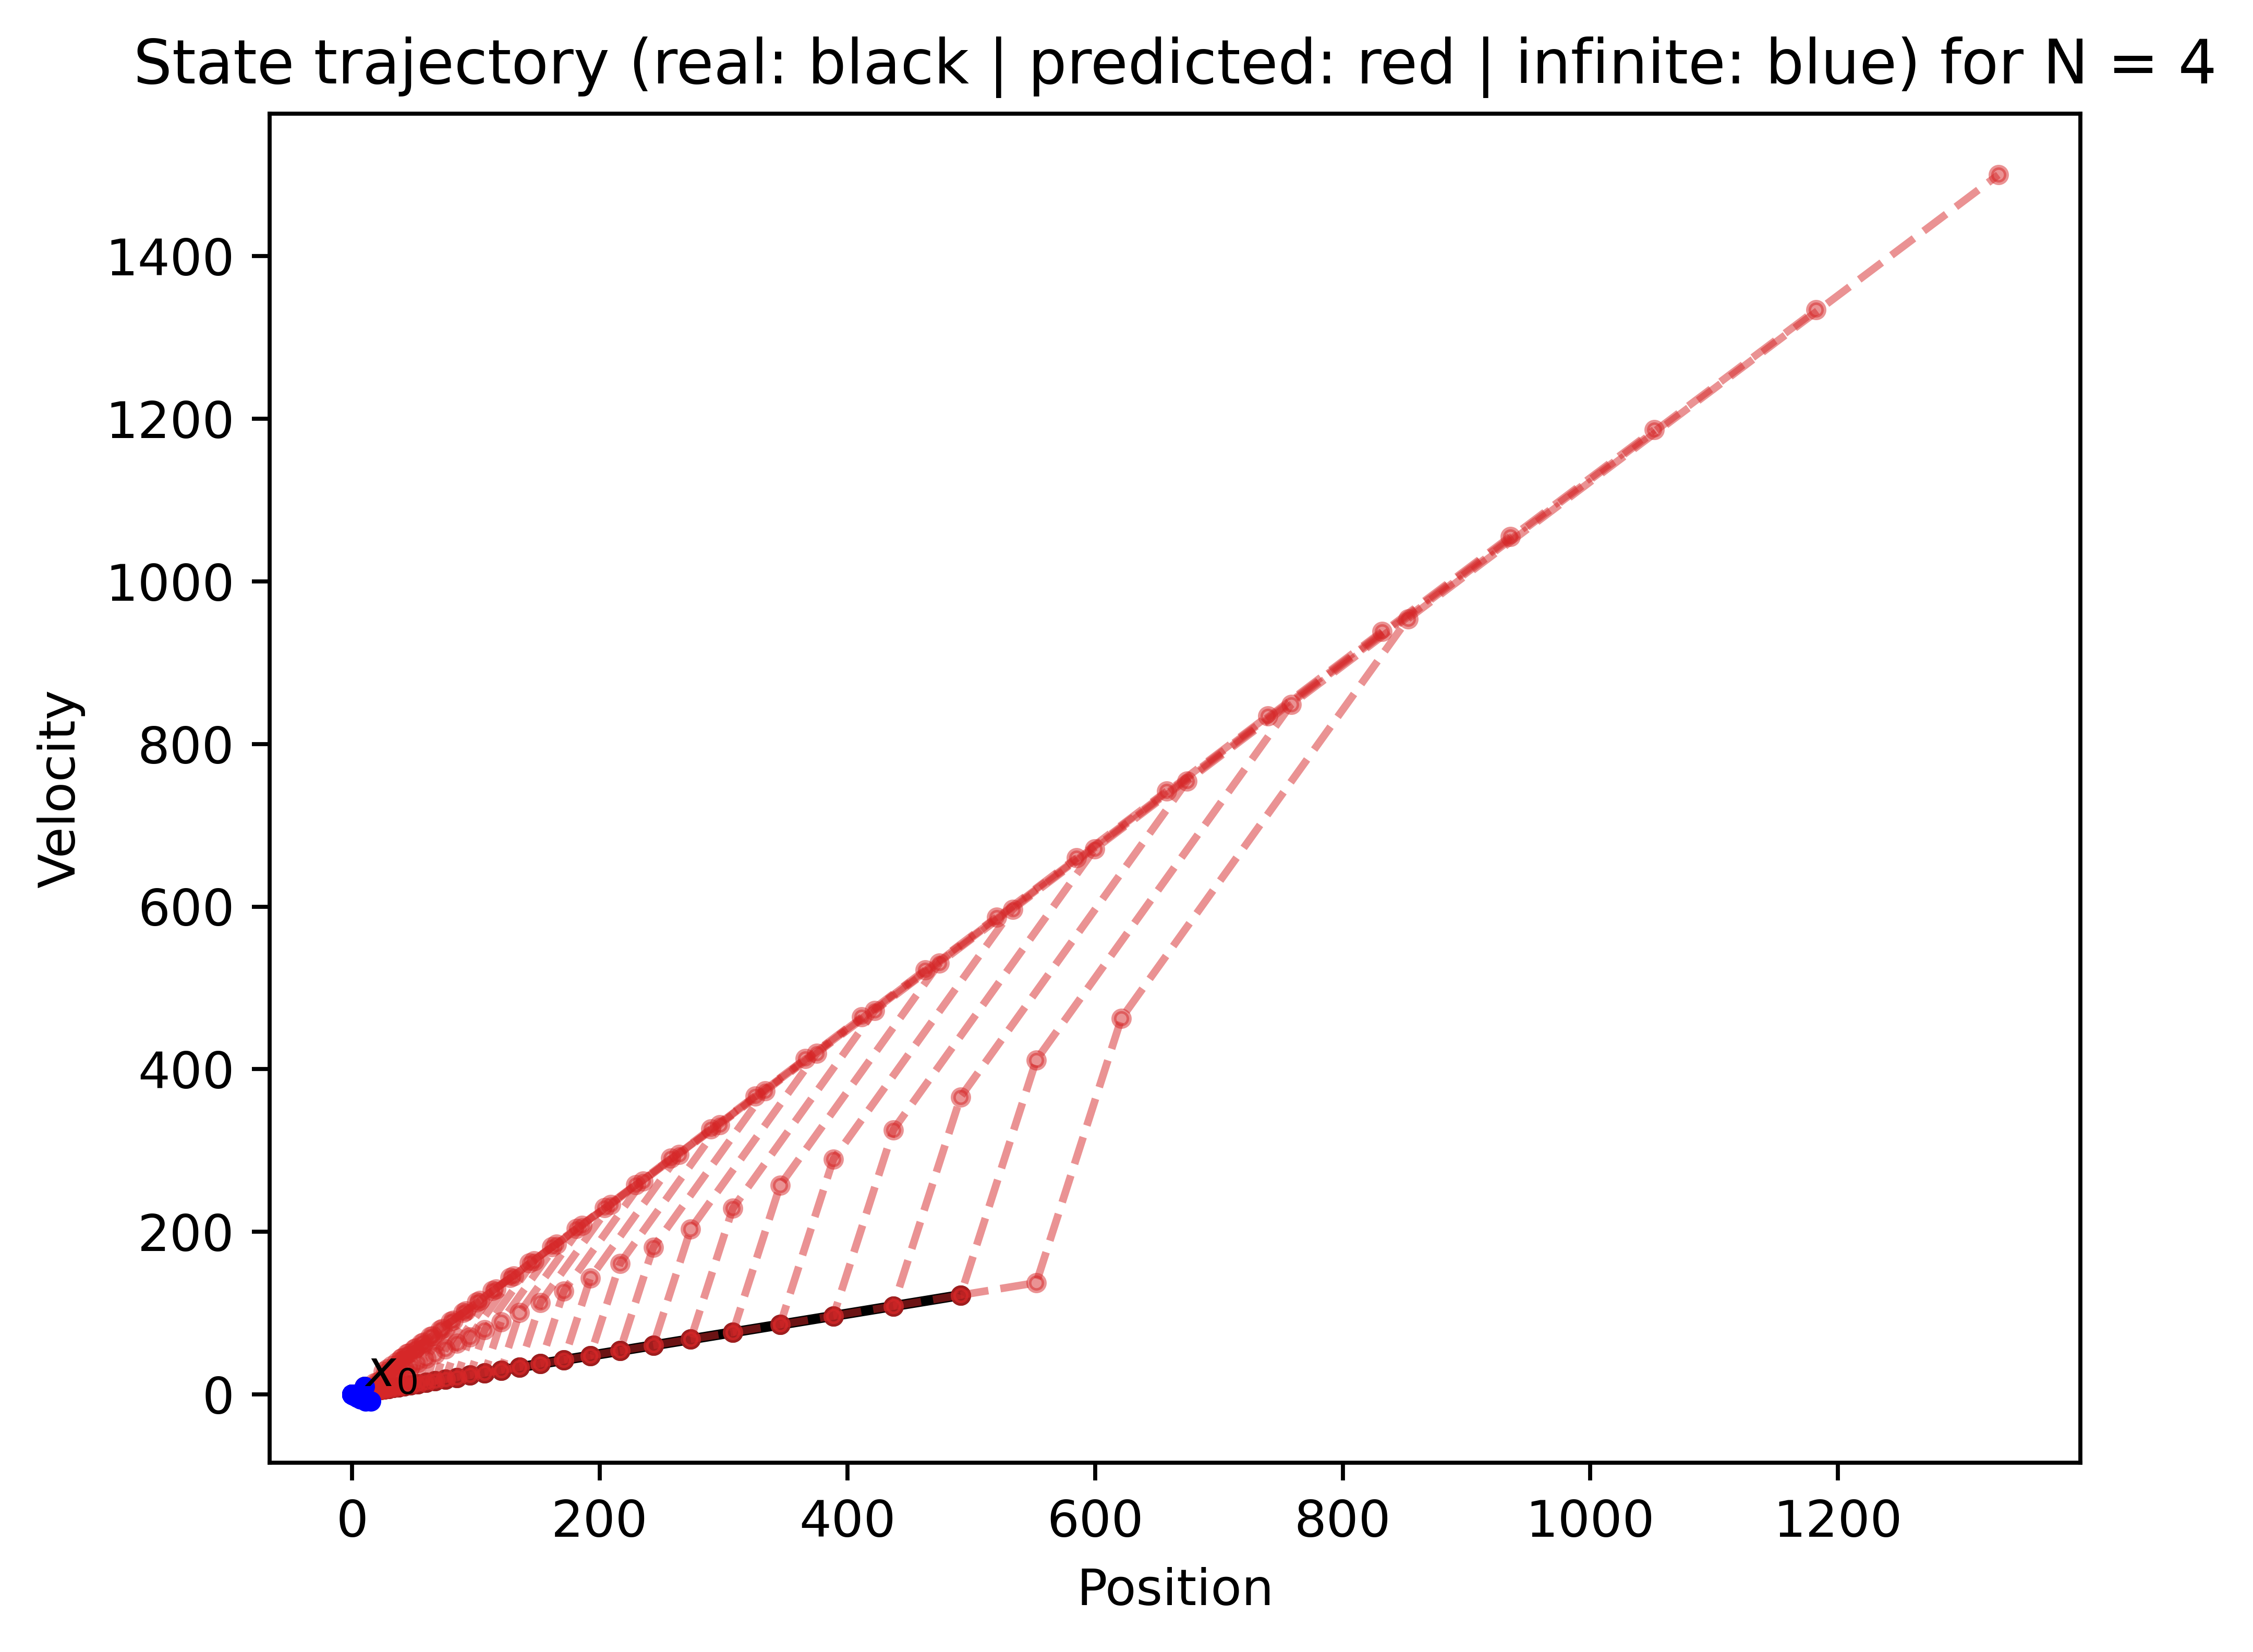
\includegraphics[width=\textwidth]{images/Assignment_11_N4.png}
			\caption{State trajectory for $N=4$}
			\label{fig:imgN4}
		\end{subfigure}
		\hfill
		\begin{subfigure}[b]{0.45\textwidth}
			\centering
			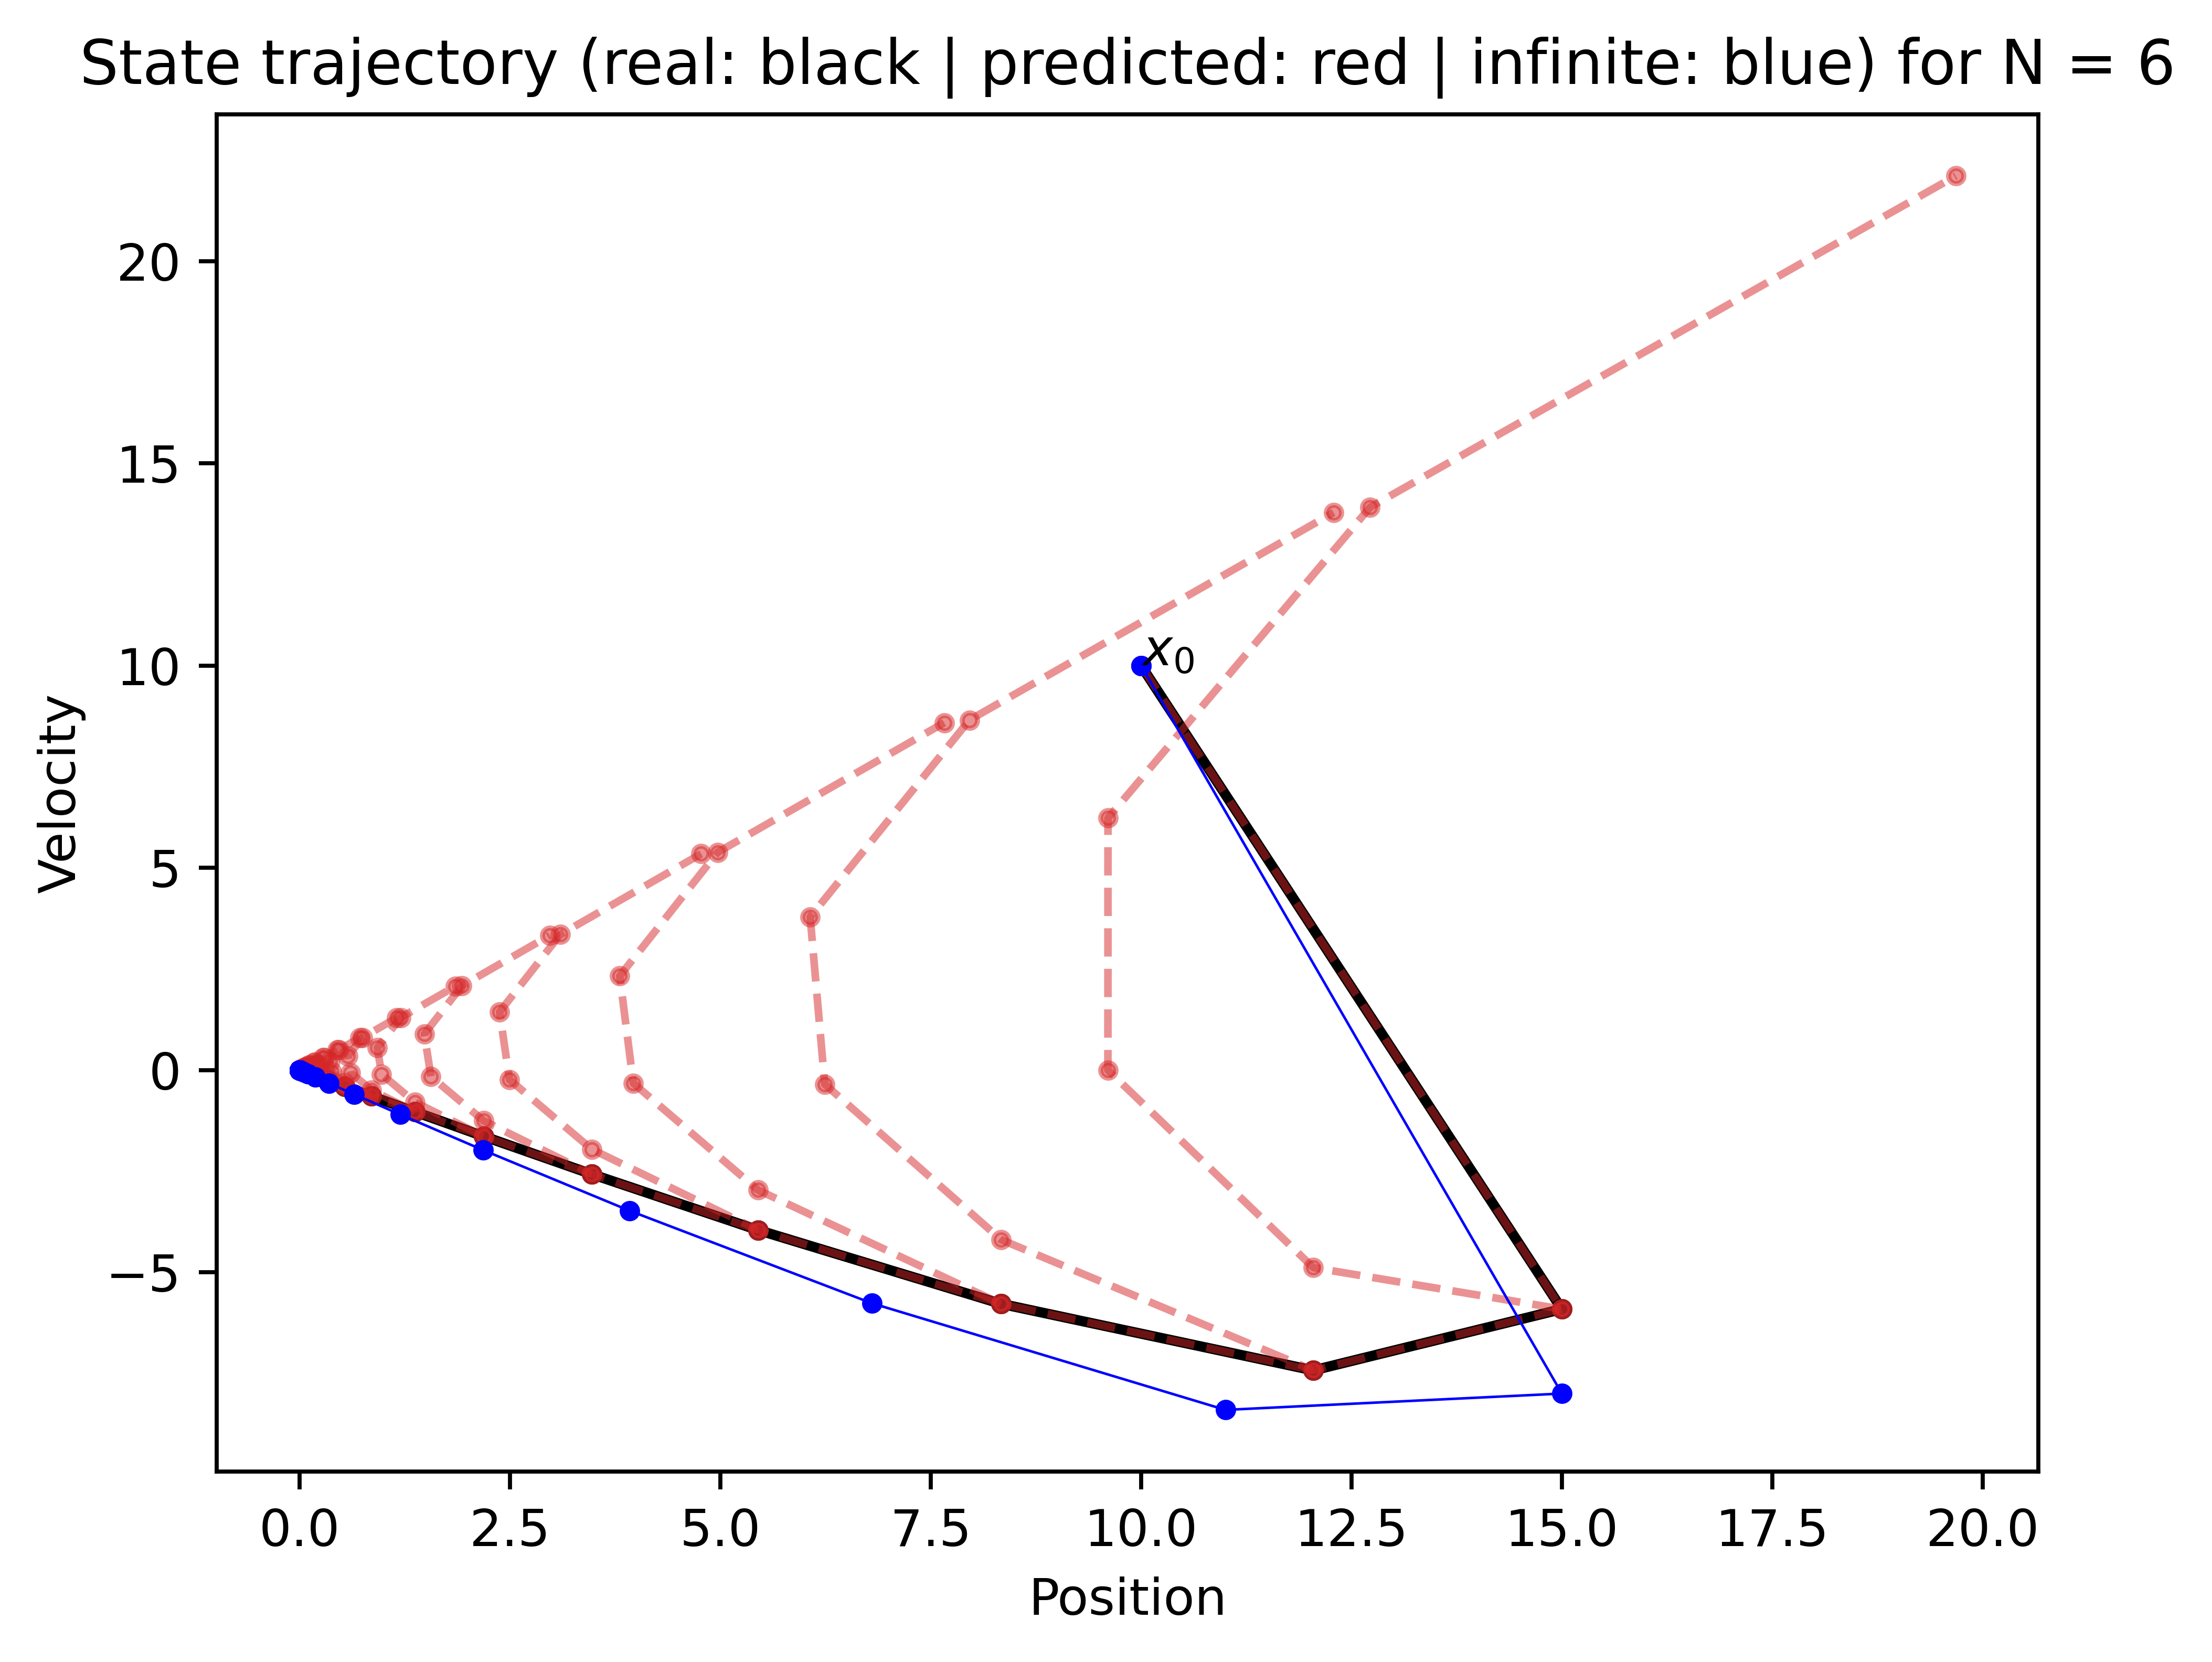
\includegraphics[width=\textwidth]{images/Assignment_11_N6.png}
			\caption{State trajectory for $N=6$}
			\label{fig:imgN6}
		\end{subfigure}
		\vfill
		\begin{subfigure}[b]{0.45\textwidth}
			\centering
			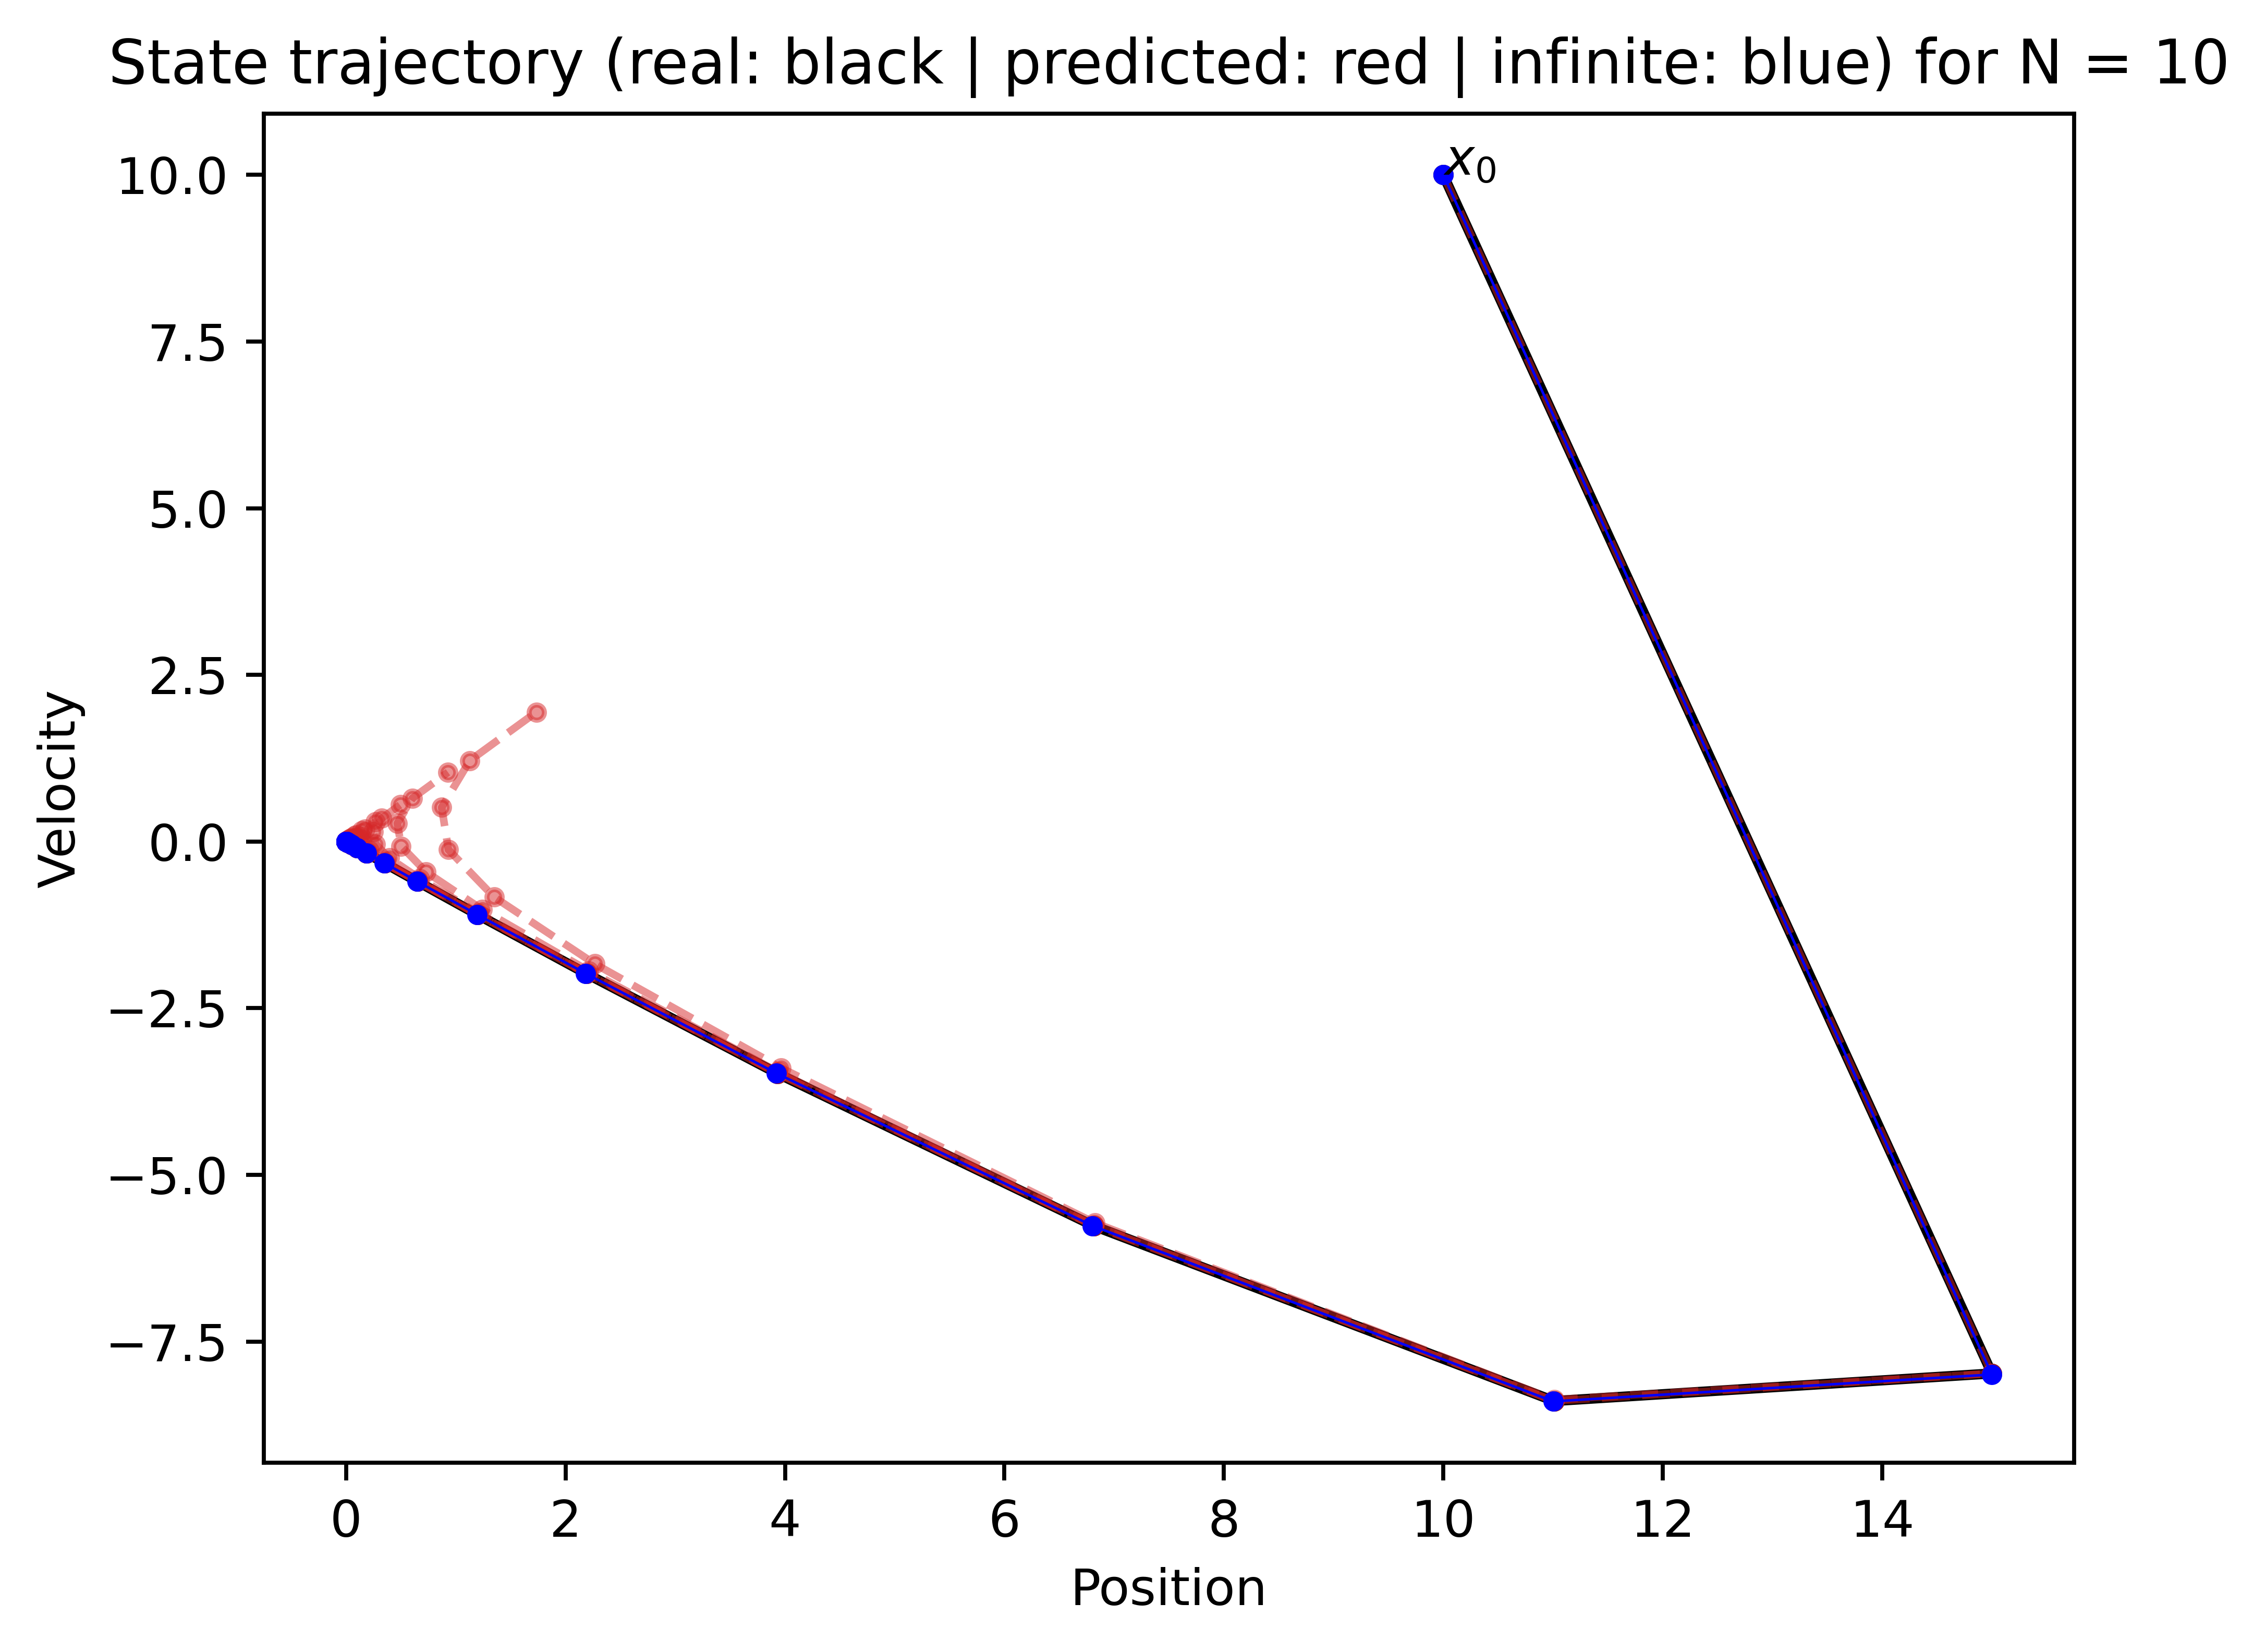
\includegraphics[width=\textwidth]{images/Assignment_11_N10.png}
			\caption{State trajectory for $N=10$}
			\label{fig:imgN10}
		\end{subfigure}
		\hfill
		\begin{subfigure}[b]{0.45\textwidth}
			\centering
			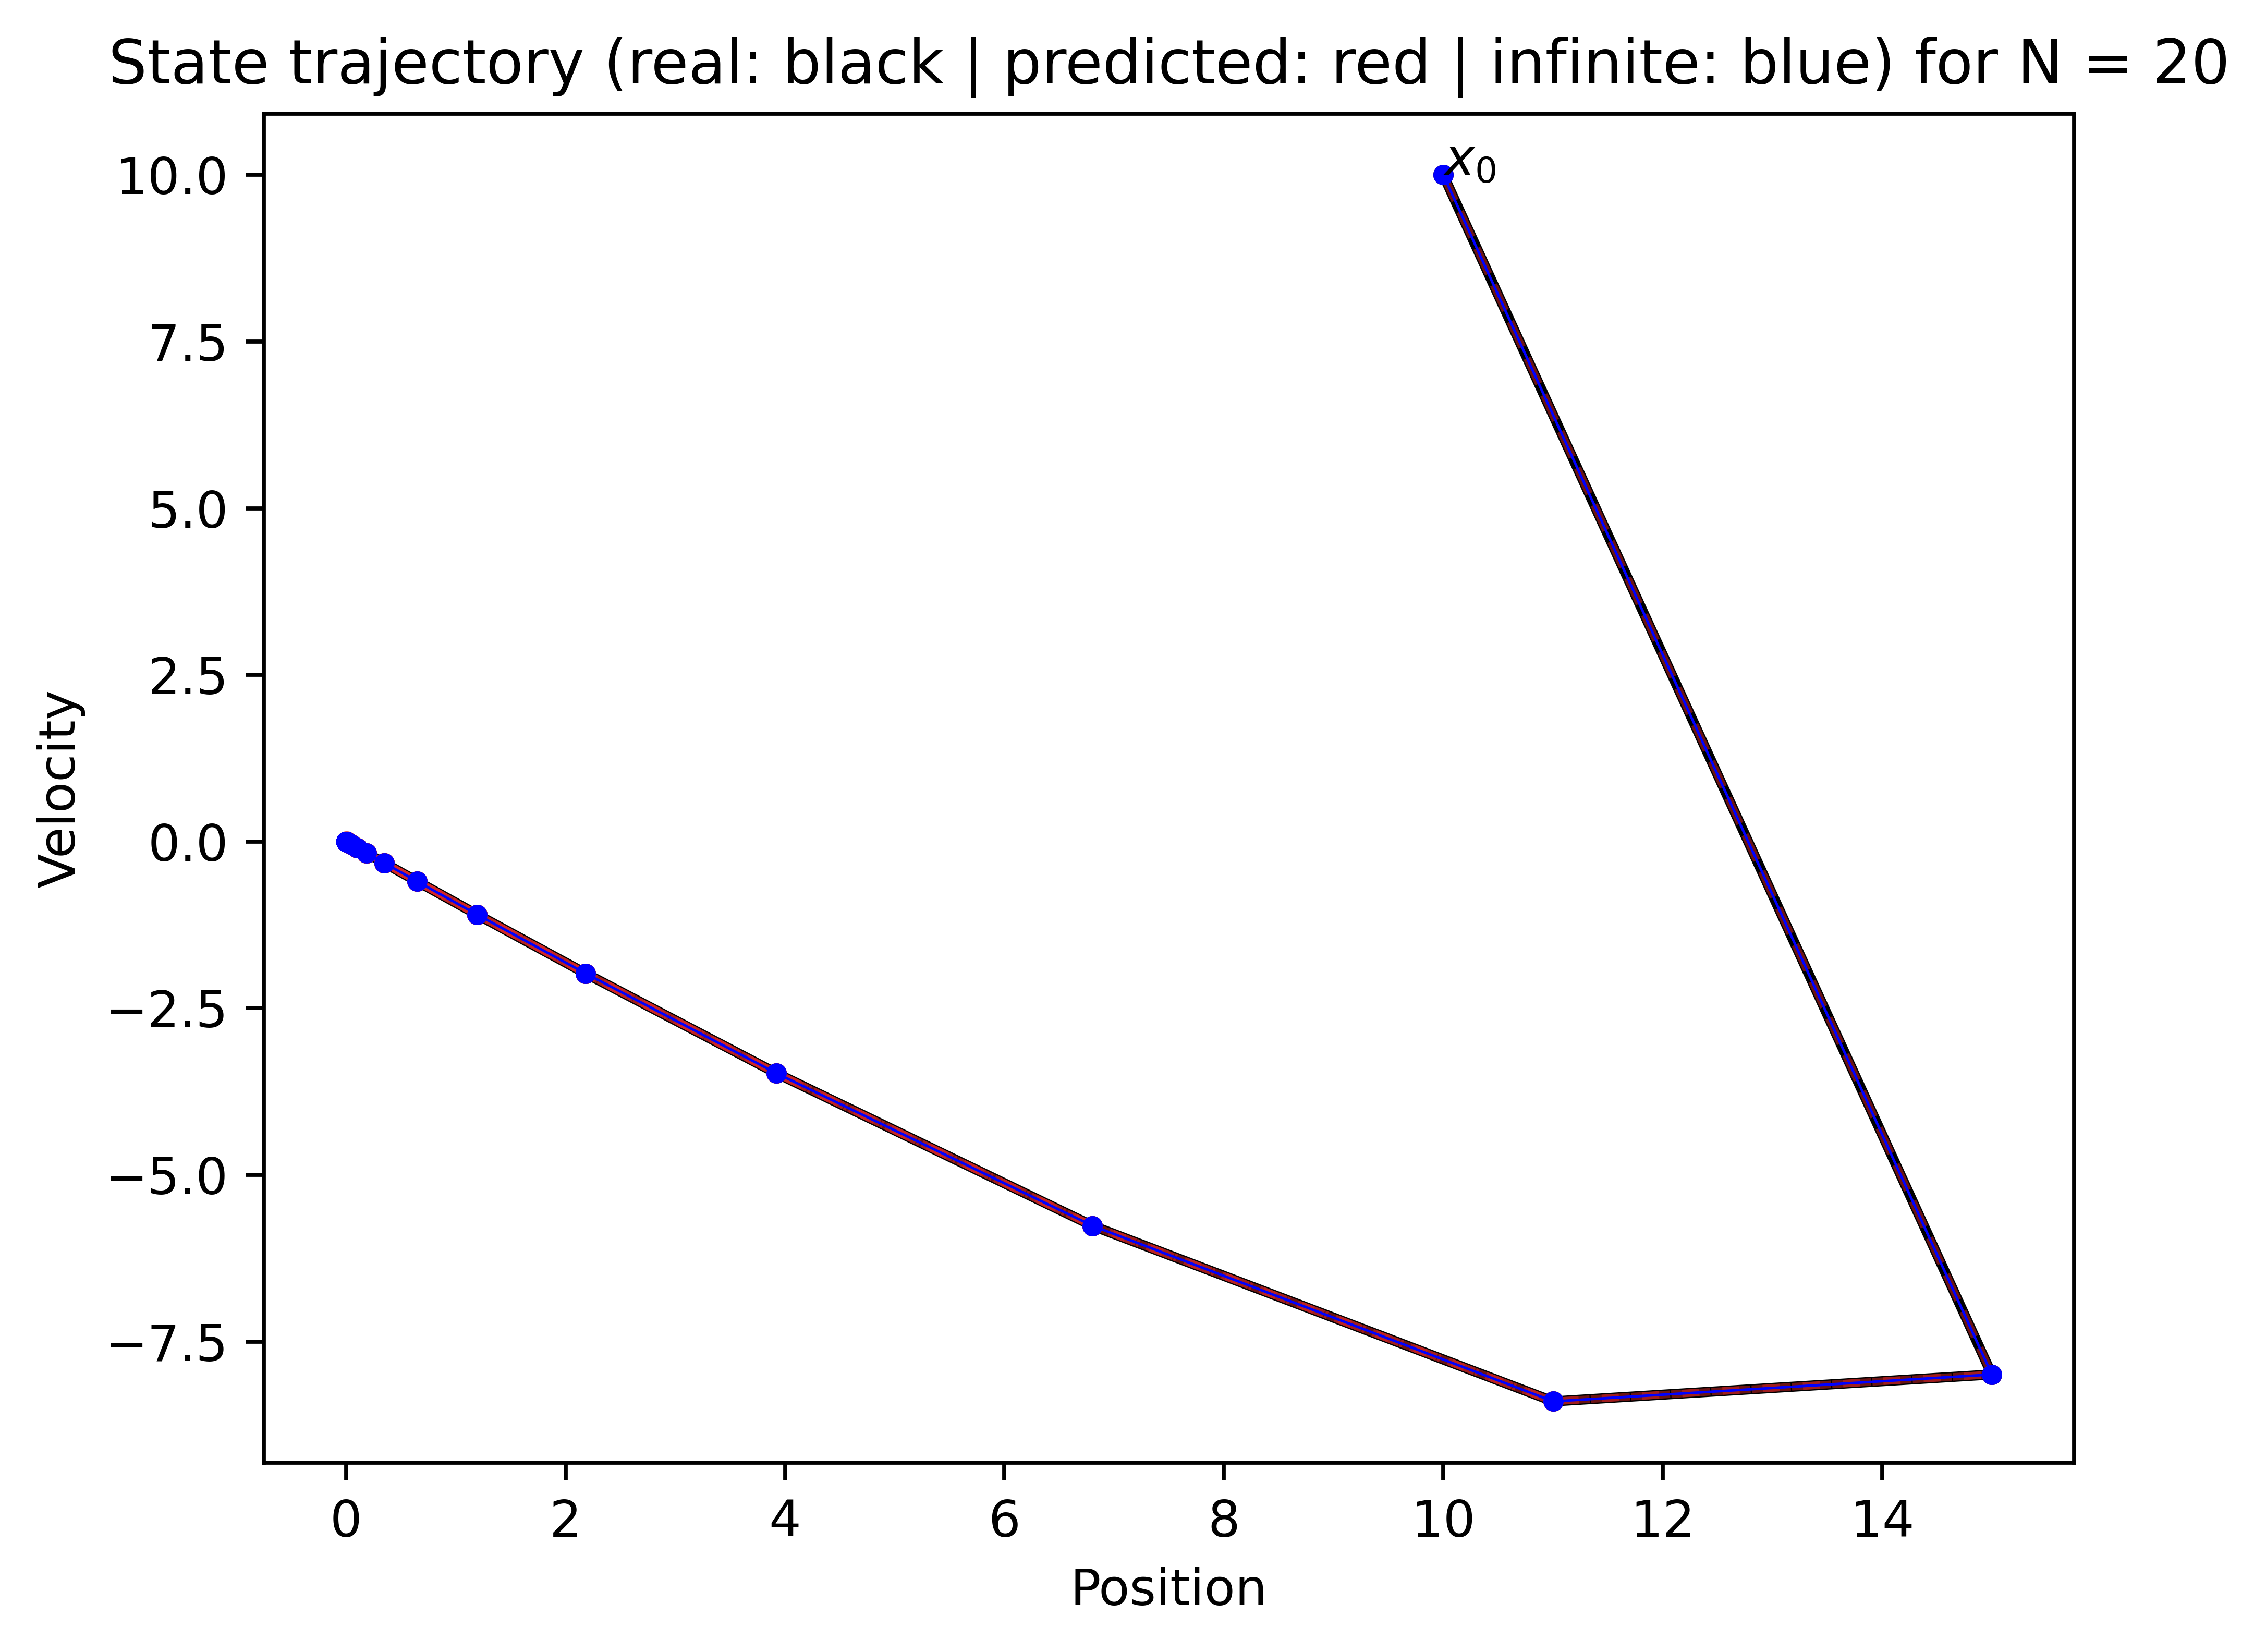
\includegraphics[width=\textwidth]{images/Assignment_11_N20.png}
			\caption{State trajectory for $N=20$}
			\label{fig:imgN20}
		\end{subfigure}
		\caption{State trajectories for different horizons}
		\label{fig:2x2grid}
	\end{figure}
\end{itemize}
For $N=4$, shown in figure \ref{fig:imgN4}, the MPC trajectories show a significant deviation from 
the infinite-horizon LQR solution. The real trajectory and predictions fail to converge toward the desired optimal behavior. 
This happens because a short prediction horizon limits the controller's ability to account for the system's long-term evolution.  

As the prediction horizon increases to $N=6$, figure \ref{fig:imgN6}, it improves noticeably. 
The predicted trajectories (red curves) begin to better align with the infinite-horizon LQR solution (blue curve), and the real trajectory starts to resemble the desired behavior. 
Although some visible deviation remains, the increased horizon length allows the controller to approximate the terminal cost more accurately, providing better foresight into the system's future behavior. 
This improvement reflects the recursive nature of the cost-to-go function: with a longer prediction horizon, the controller reduces the mismatch between the finite-horizon cost approximation and the true long-term cost-to-go.

For N=10, figure \ref{fig:imgN10}, the finite-horizon MPC achieves near-optimal behavior, as evidenced by the close overlap between the real and predicted trajectories with the infinite-horizon LQR trajectory. 
At this horizon length, the MPC solution has almost converged to the optimal control law. 
The terminal cost and the resulting feedback gain closely approximate those obtained from solving the Discrete Algebraic Riccati Equation (DARE), which characterizes the infinite-horizon optimal solution. 

As N increases, figure \ref{fig:imgN20} shows a simulation where $N=20$, the terminal cost used in the finite-horizon MPC converges to the true cost-to-go, enabling the MPC to replicate the infinite-horizon behavior.

\begin{assignment}
	Numerically compare the quality of the finite-horizon LQR controller to the infinite horizon controller. 
	For the same fixed $x_0$ as before and for $N$ ranging from 1 to 10\footnote{\textbf{Hint:} manually set the $y$-limit of the plot to $[0, 2000]$. Otherwise, the costs of unstable controllers will dominate the figure.}: 
\begin{itemize}
	\item Plot $V_{N} = x_0^\top P_N x_0$ versus $N$
	\item Plot $V_{\infty} = x_0^\top P_{\infty} x_0$ on the same axis (this is just a horizontal line).
	\item Approximate the infinite horizon cost for the finite-horizon controller using a long state and input trajectory:
		\begin{align} \nonumber
			\hat{V}_{N} = \sum_{k=0}^\infty(x_k^\top Q x_k + x_k^\top K^\top R K x_k) \approx \sum_{k=0}^{100}(x_k^\top Q x_k + x_k^\top K^\top R K x_k). 
		\end{align}
	and add a plot of $\hat{V}_N$ vs. $N$ on the same figure.
	\item Describe what you observe: Do you observe convergence? Which quantities observe to which and in what direction? \textbf{Briefly} explain these observations.
\end{itemize}
\end{assignment}

\begin{flushleft}
Figure \ref{fig:assignment1_2} illustrates the behavior of the value function $ V_N $, $ V_\infty $ and $ \hat{V}_N $ as a function of the horizon $ N $.
Each curve represents a different computation of the cost. $ V_N $, shown in cyan, which is converging from below represents the cost of following the MPC policy over a finite horizon 
$ N $. Since it only considers the cost over the horizon without accounting for what happens beyond it, $V_N$ tends to underestimate the total cost. As $N$ increases, $V_N$ includes the effects of more steps and approaches the infinite-horizon cost $V_\infty$.
The value function $\hat{V}_N$, shown in green, represents the cost computed for the infinite sequence of actions when applying the MPC policy derived using horizon $N$.
Initially, for small horizons (e.g. $N$ < 4), the MPC policy produces an unstable trajectory, leading to an infinite cost. However, as $N$ increases, the policy stabilizes, and 
$\hat{V}_N$ converges from above to the infinite-horizon cost $V_\infty$. The magenta line represents the infinite-horizon optimal cost $V_\infty$, which is constant and provides a benchmark for comparison.  
\end{flushleft}

The figure highlights the importance of selecting an adequate prediction horizon in MPC. For small horizons, the controller may produce unstable trajectories, as evidenced by the infinite cost. Once the horizon is sufficiently long (e.g. $N \geq$ 4), the MPC policy stabilizes, and both $V_N$ and $\hat{V}_N$ approach $V_\infty$, ensuring optimal and stable control.
\begin{figure}[H]
    \centering
    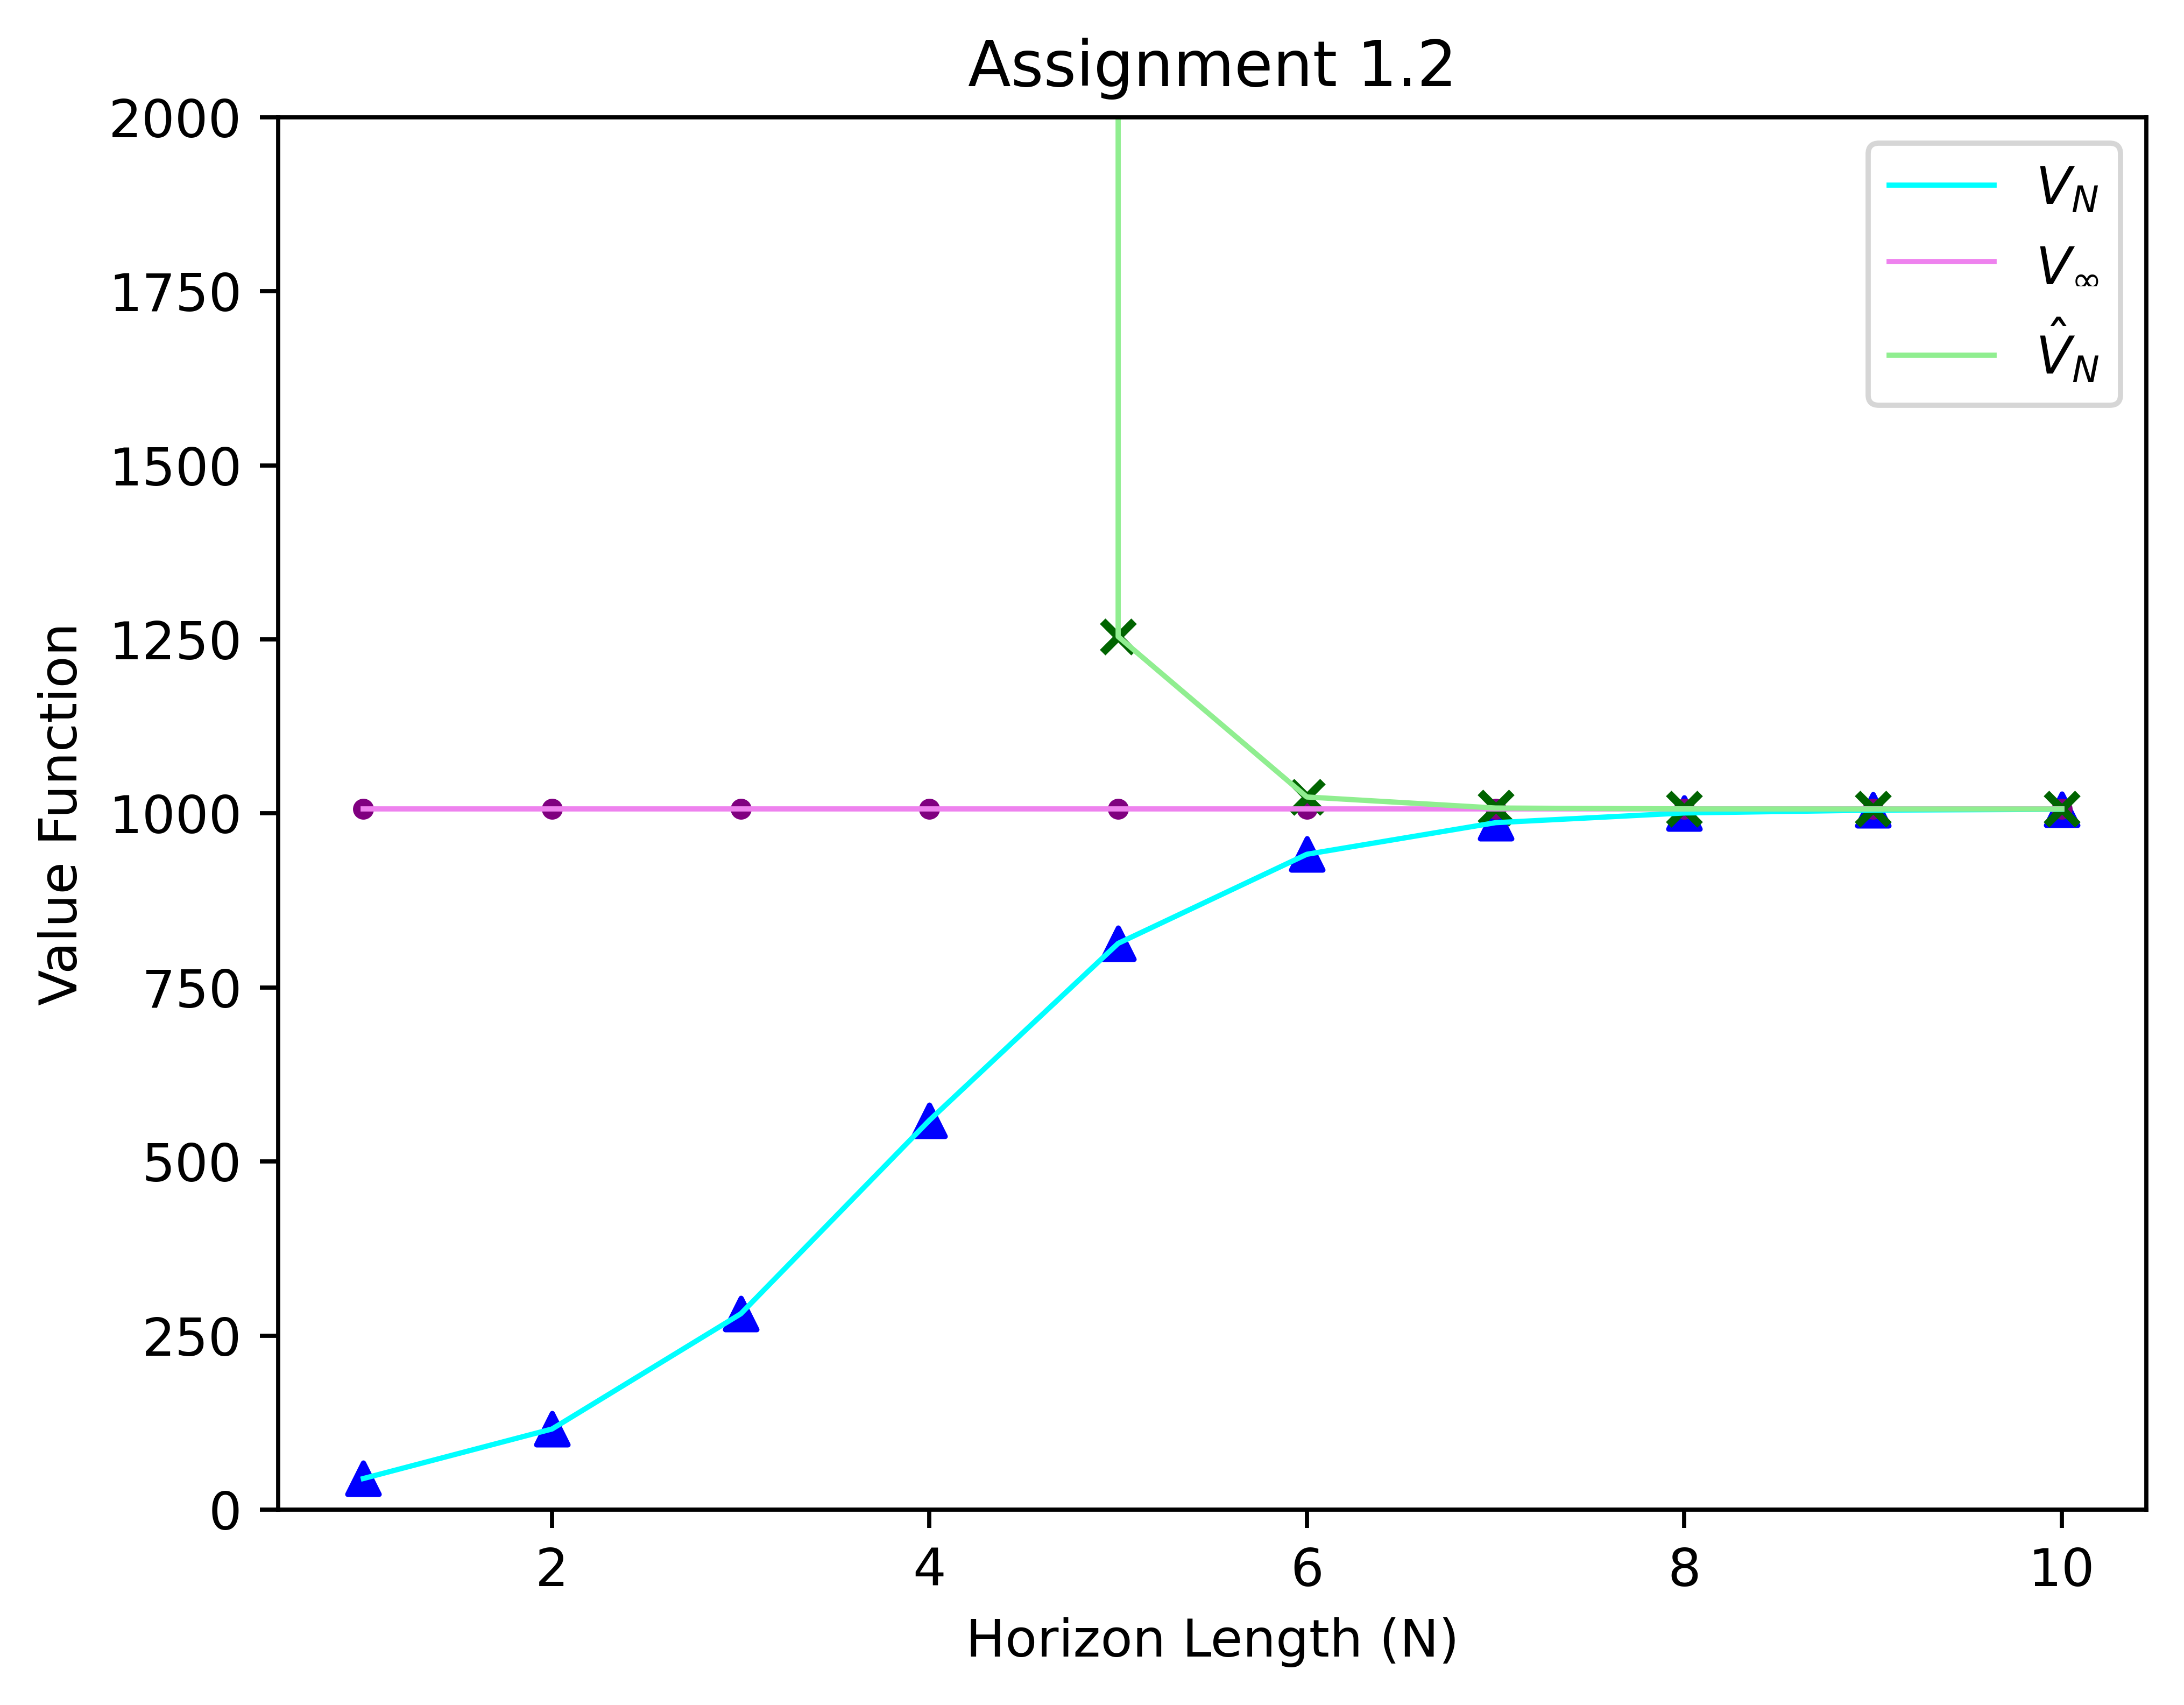
\includegraphics[width=0.7\textwidth]{images/Assignment_12.png}
    \caption{Plot}
    \label{fig:assignment1_2}
\end{figure}



\newpage
\section{Linear MPC and convex optimization}
\textbf{See the session 2 sheet for the set-up.}

The goal of this assignment is to look more closely at what goes wrong in the 
final exercise of the session, and to gain some intuition about ways to fix it.
In essence, the problem that occurs is a symptom of the myopic nature of MPC,
that is, it can only take into account what happens in the very near future.
To rectify this, we have to provide it with information about the long-term
behavior of the system under the applied controls.

\textbf{Remark.} The assignments in this session should be performed in discrete time.

\begin{assignment}
	Consider the vehicle at a fixed position and velocity $(p_0, v_0)$.
	Suppose we apply the maximum brake, i.e., $u_t = u_{\min}$ for $t = 0, \dots, T$.
	Write an expression of $T$ as a function of $v_0$, such the vehicle can come to standstill in $T$ steps.
\end{assignment}

\begin{flushleft}
Given the system dynamics:
\begin{equation}
	\begin{aligned}
		&x_{t+1} = \begin{bmatrix}
			1 & T_s \\ 
			0 & 1
		\end{bmatrix} x_t +
		\begin{bmatrix}
			0 \\ T_s
		\end{bmatrix} u_t \\
		&\text{where } x_t = \begin{bmatrix}
			p_t \\ 
			v_t
		\end{bmatrix}
	\end{aligned}
\end{equation}
it is possible to develop the evolution of the state's elements over time:
\end{flushleft}
\begin{equation}
	\begin{cases}
		p_1 = p_0 + T_s v_0 \\
		v_1 = v_0 + T_S u_{min}
	\end{cases}
\end{equation}
\begin{equation}
	\begin{cases}
		p_2 = p_1 + T_s v_1 = p_0 + 2 T_s v_0 + T_s^2 u_{min} \\
		v_2 = v_1 + T_S u_{min} = v_0 + 2 T_s u_{min}
	\end{cases}
\end{equation}
Therefore we have that:
\begin{equation}
	\begin{cases}
		p_T = p_{T-1} + T_s v_{T-1} = p_0 + T_s v_0 T + \frac{1}{2} T (T-1) T_s^2 u_{min} \\
		v_T = v_0 + T_s T u_{min}
	\end{cases}
\end{equation}
Since the objective is for the vehicle to come to a standstill in T steps:
\begin{equation}
	v_T = v_0 + T_s T u_{min} = 0 \implies T = -\frac{v_0}{T_s u_{min}}
\end{equation}



\begin{assignment}
	For a given $T$, compute the total braking distance, i.e., the distance travelled during the 
	deceleration: $p_T - p_0$. 
\end{assignment}

\begin{flushleft}
As previously stated, the vehicle's position after T steps can be expressed as:
\end{flushleft}
\begin{equation}
		p_T = p_{T-1} + T_s v_{T-1} = p_0 + T_s v_0 T + \frac{1}{2} T (T-1) T_s^2 u_{min}
\end{equation}
Therefore, the total braking distance is given by the difference between the final and initial positions:
\begin{equation}
		p_T - p_0 = T_s v_0 T + \frac{1}{2} T (T-1) T_s^2 u_{min}
\end{equation}




\begin{assignment}\label{ex:sess2-constraint}
   Use the result of the previous exercises to formulate a constraint on a state $x = (p, v)$ that 
   will guarantee that there will always exist a control input that will keep future states 
   in the set $S = \{x \mid p \leq p_{\max}\}$.
\end{assignment}

\begin{flushleft}
	Given the total braking distance expression derived in the previous exercise, where T can be expressed as a function of the initial velocity $v_0$, we can reformulate the total breaking distance as follows:
\end{flushleft}
\begin{equation}
	\begin{aligned}
		p_T - p_0 &= \frac{-v_0}{T_s u_{min}} T_s v_0 + \frac{1}{2} \Bigg(\frac{-v_0}{T_s u_{min}}\Bigg) \Bigg(\frac{-v_0}{T_s u_{min}}-1\Bigg) T_s^2 u_{min} \\
				  &= \frac{-v_0^2}{u_{min}} + \frac{1}{2} v_0 \Bigg( \frac{v_0 + T_s u_{min}}{u_{min}}\Bigg) 
	\end{aligned}
\end{equation}
Therefore, the constraint that guarantees that there will always exist a control input that will keep future states in the set $S$, states within the breaking distance to $p_{max}$, is:
\begin{equation}
	\begin{aligned}
		p_0 + (p_T - p_0) &\leq p_{max} \\
		p_0 \leq p_{max} - (p_T - p_0) &= p_{max} + \frac{v_0^2}{u_{min}} - \frac{1}{2} v_0 \Bigg( \frac{v_0 + T_s u_{min}}{u_{min}}\Bigg)
	\end{aligned}
\end{equation}



\begin{assignment} \label{ex:extra-1}
	Write a function that takes the horizon $N$ as an input and that 
	for all initial states $[-10, 0] \leq x_0 \leq [1, 25]$ (sampled in a grid), checks whether your MPC controller is feasible at this initial state.
	Set $u_{\min} = -5$.
	Leave the other settings at the same values as the ones in the session.
	For all $N \in \{2, 5, 10\}$, make a plot showing the set of states that are feasible (this can be a simple scatter plot), 
	and draw the boundary of the constraint you derived in \cref{ex:sess2-constraint}. 
	\textbf{Remark.} You only have to check the initial feasibility of the MPC problem, not recursive feasibility.
\end{assignment}
\begin{flushleft}
	The blue curve, in figure \ref{fig:assignment2_4_1}, \ref{fig:assignment2_4_2} and \ref{fig:assignment2_4_3}, represents the derived constraint, denoting the boundary for feasible initial points given the initial velocities. 
	States below this boundary ensure that the vehicle can decelerate and come to a complete stop within the allowed constraints, having a maximum final position $p_{max}=1$. 
	Thus, it is expected that only states below this line are classified as feasible initial states, as they satisfy the physical and control limitations of the system.
\end{flushleft}
From figure \ref{fig:assignment2_4_1}, \ref{fig:assignment2_4_2} and \ref{fig:assignment2_4_3} can be seen that the number of feasible initial states decreases as the prediction horizon $N$ increases. 
This phenomenon arises because, with a longer prediction horizon, the Model Predictive Control algorithm accounts for future constraints over a longer period. 
Specifically, the system becomes increasingly aware that with the minimum allowable braking input of $u_{min}=-5$, the car will not be able to stop in time if the initial velocity exceed a certain threshold, blue line, with respect to the initial position.
\begin{figure}[H]
    \centering
    \begin{minipage}{0.7\textwidth}
        \centering
        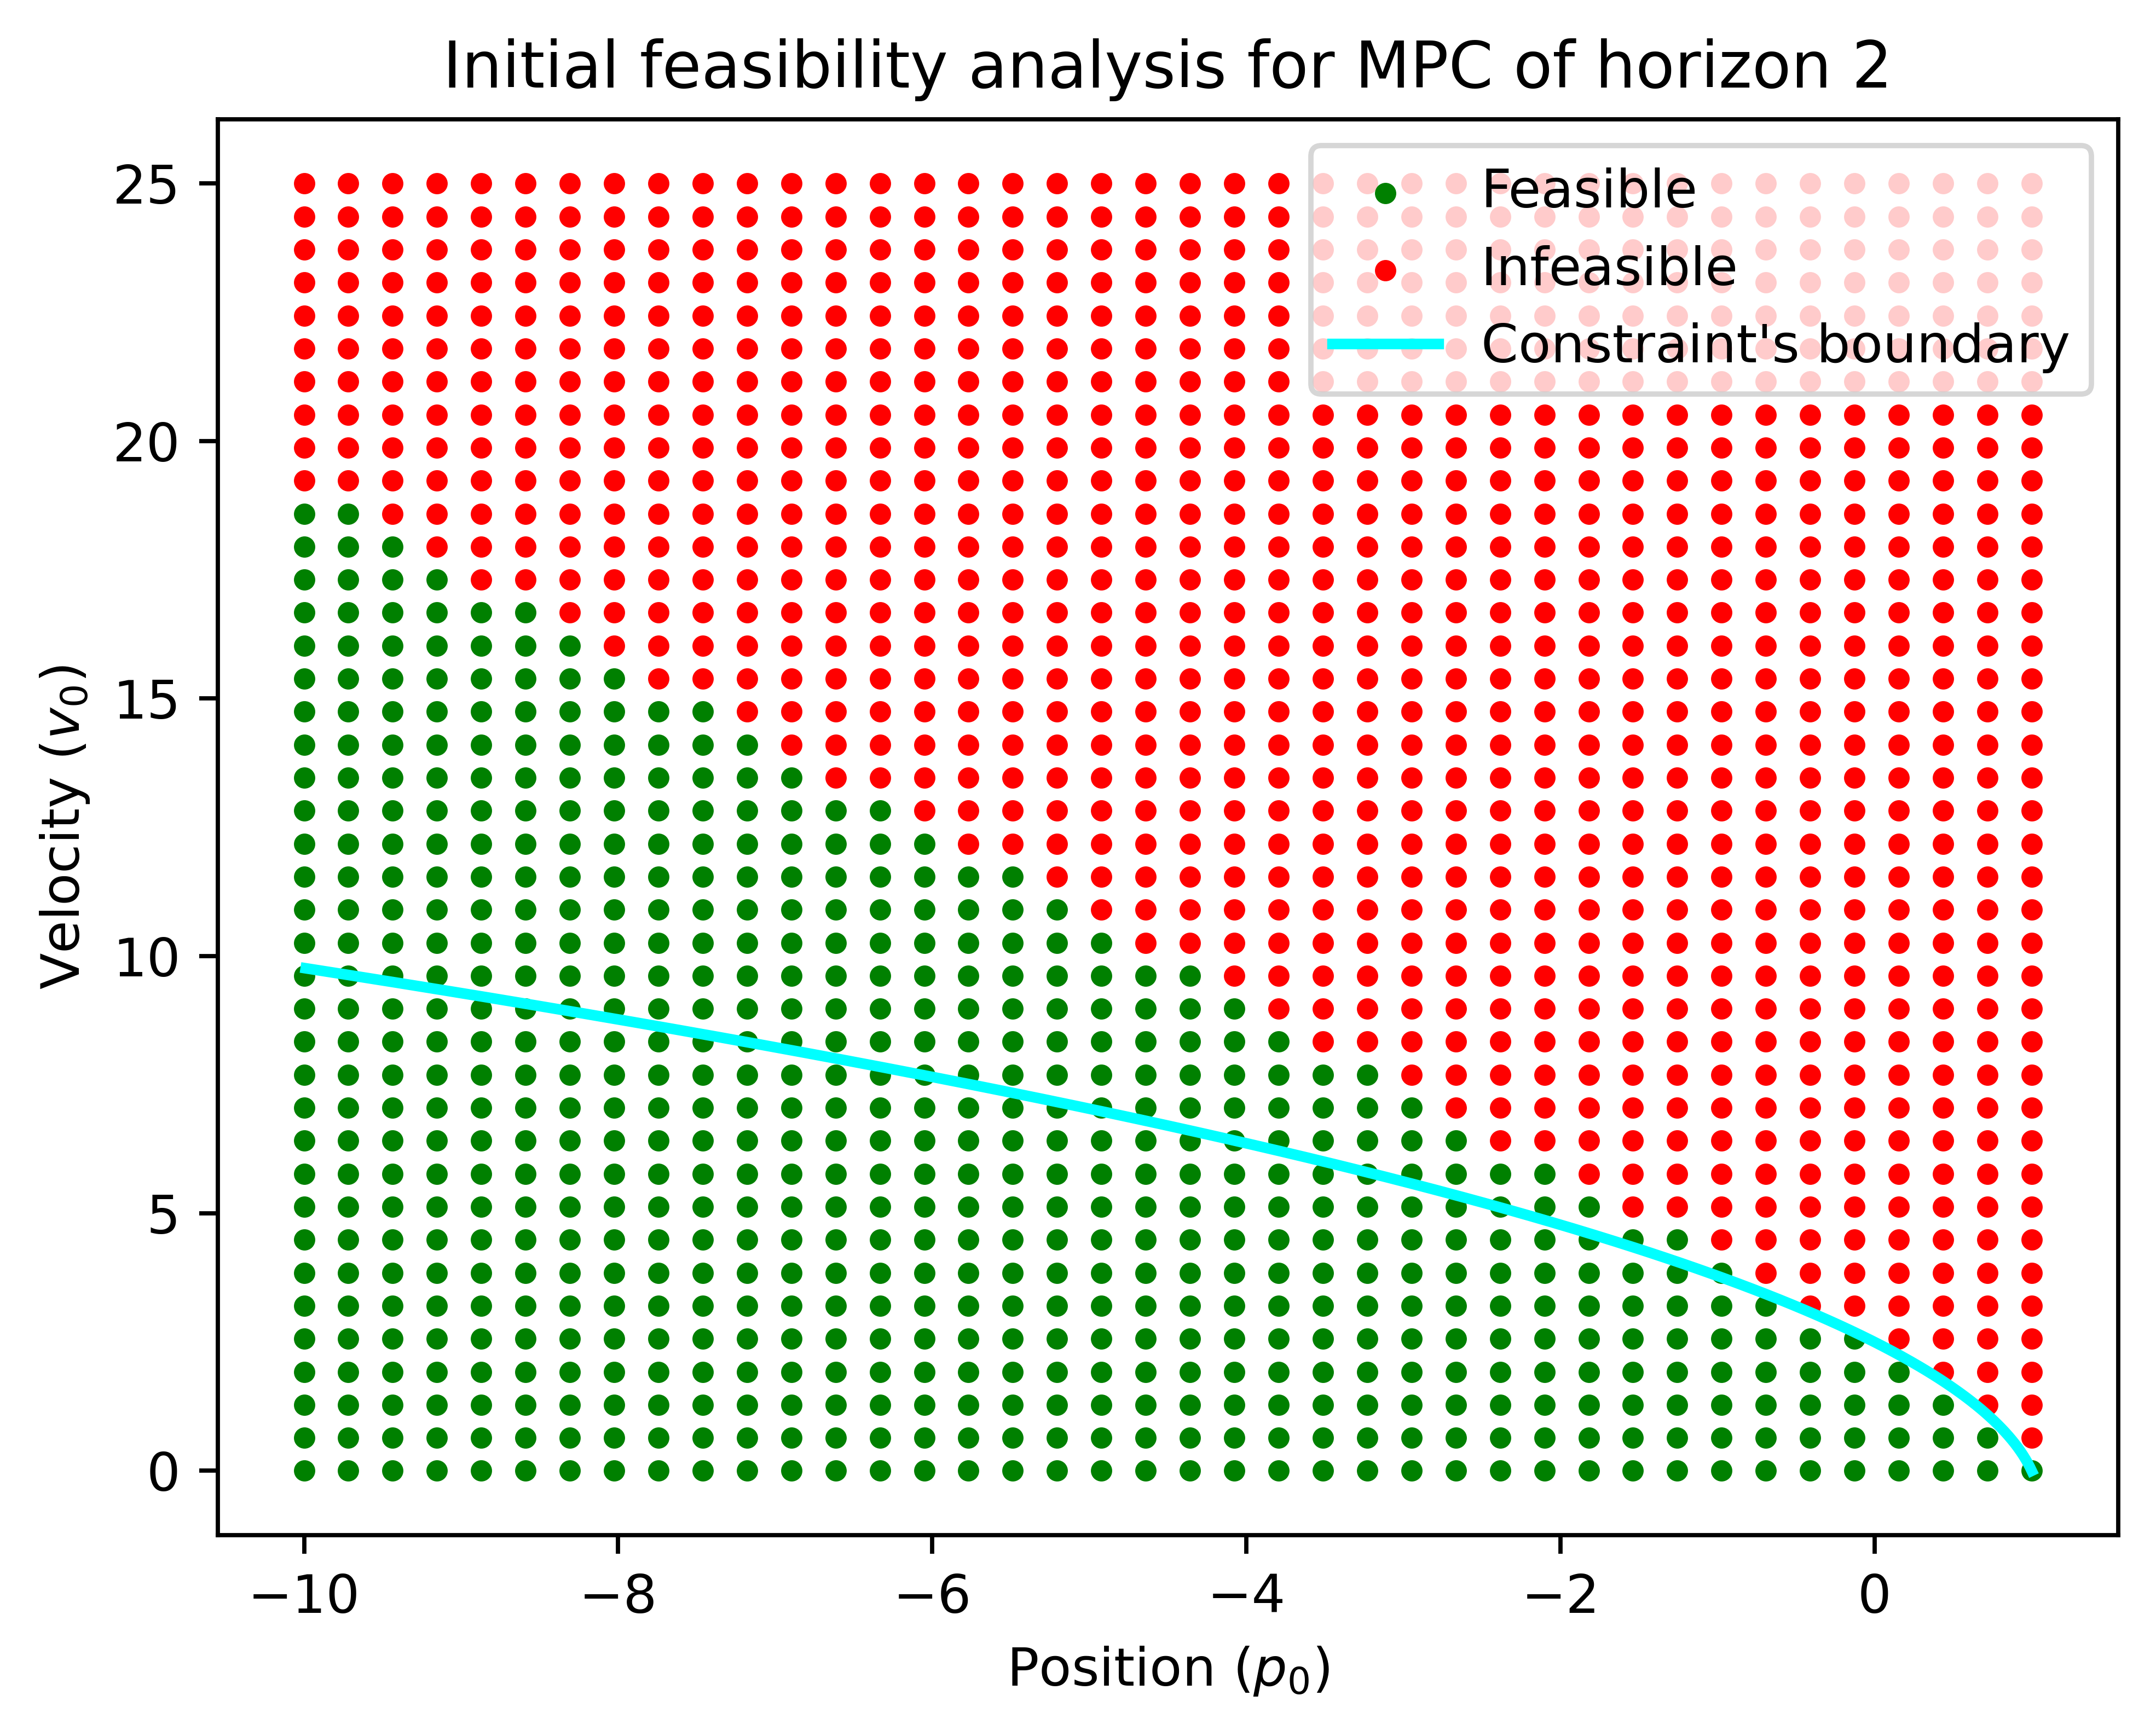
\includegraphics[width=\textwidth]{images/Assignment_24_N2.png}
        \caption{$N$ = 2}
        \label{fig:assignment2_4_1}
    \end{minipage}
    \hfill
    \begin{minipage}{0.7\textwidth}
        \centering
        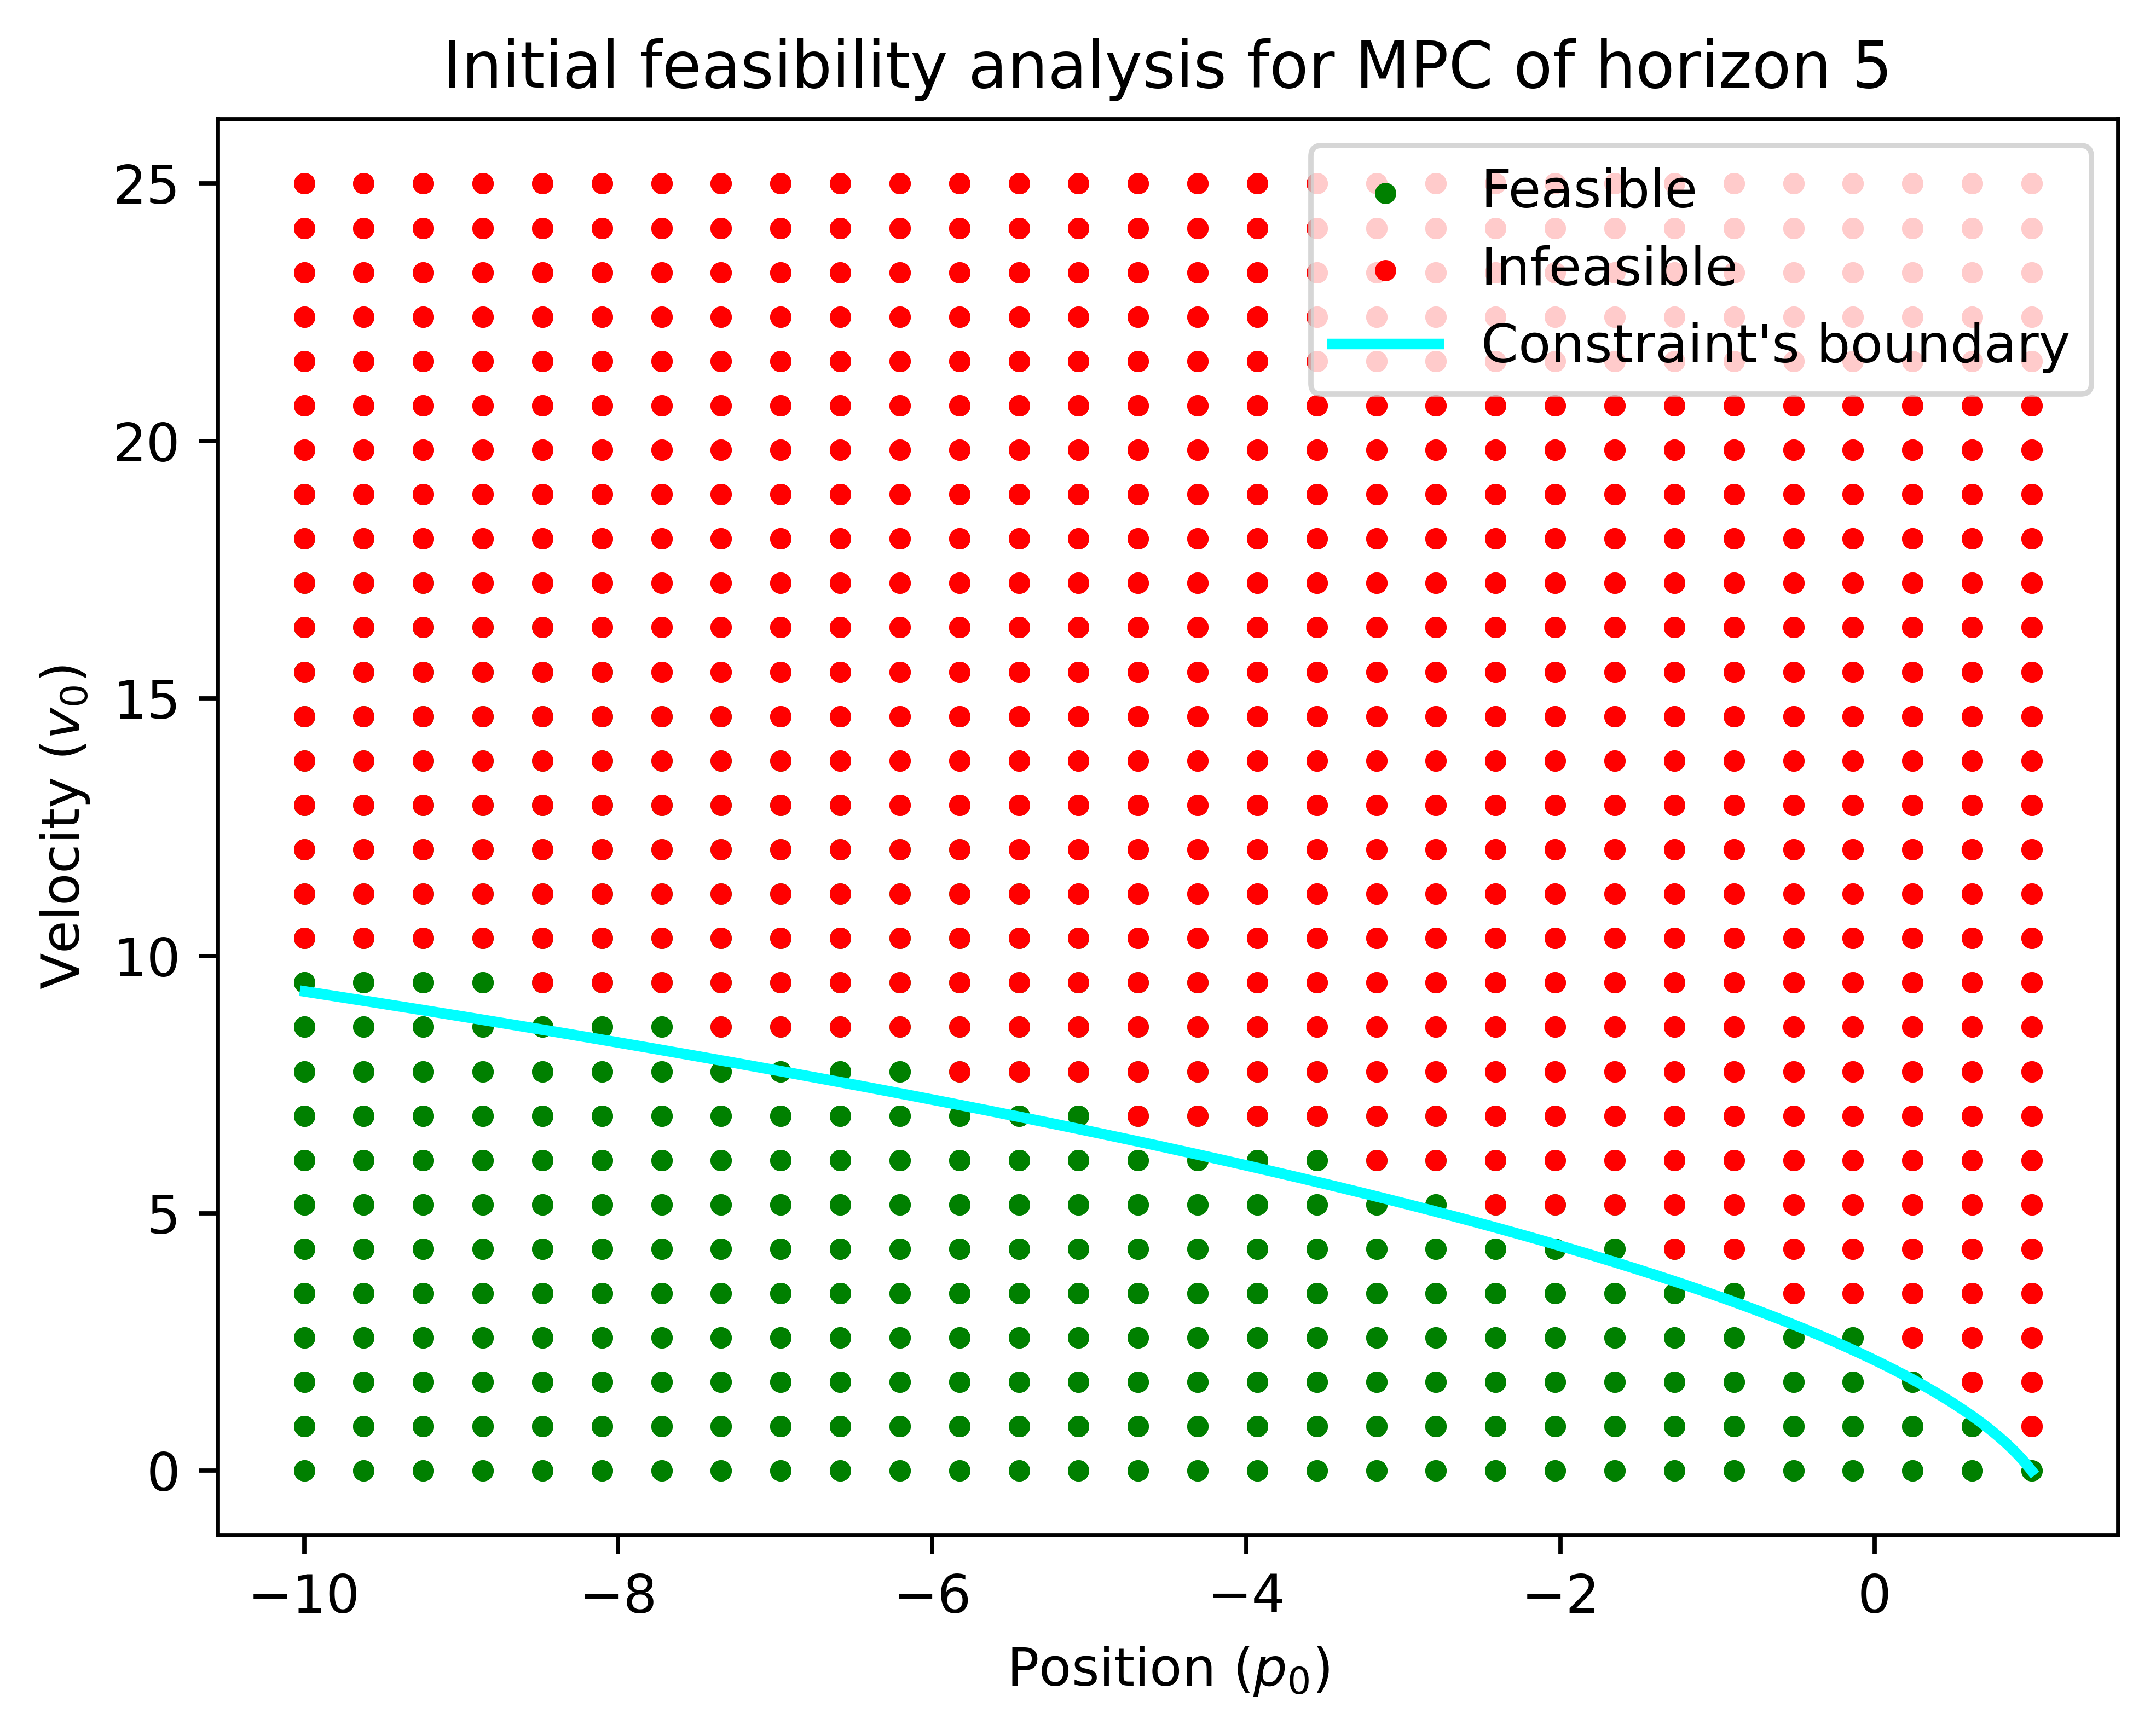
\includegraphics[width=\textwidth]{images/Assignment_24_N5.png}
        \caption{$N$ = 5}
        \label{fig:assignment2_4_2}
    \end{minipage}
\end{figure}
\begin{figure}[H]
    \centering
    \begin{minipage}{0.7\textwidth}
        \centering
        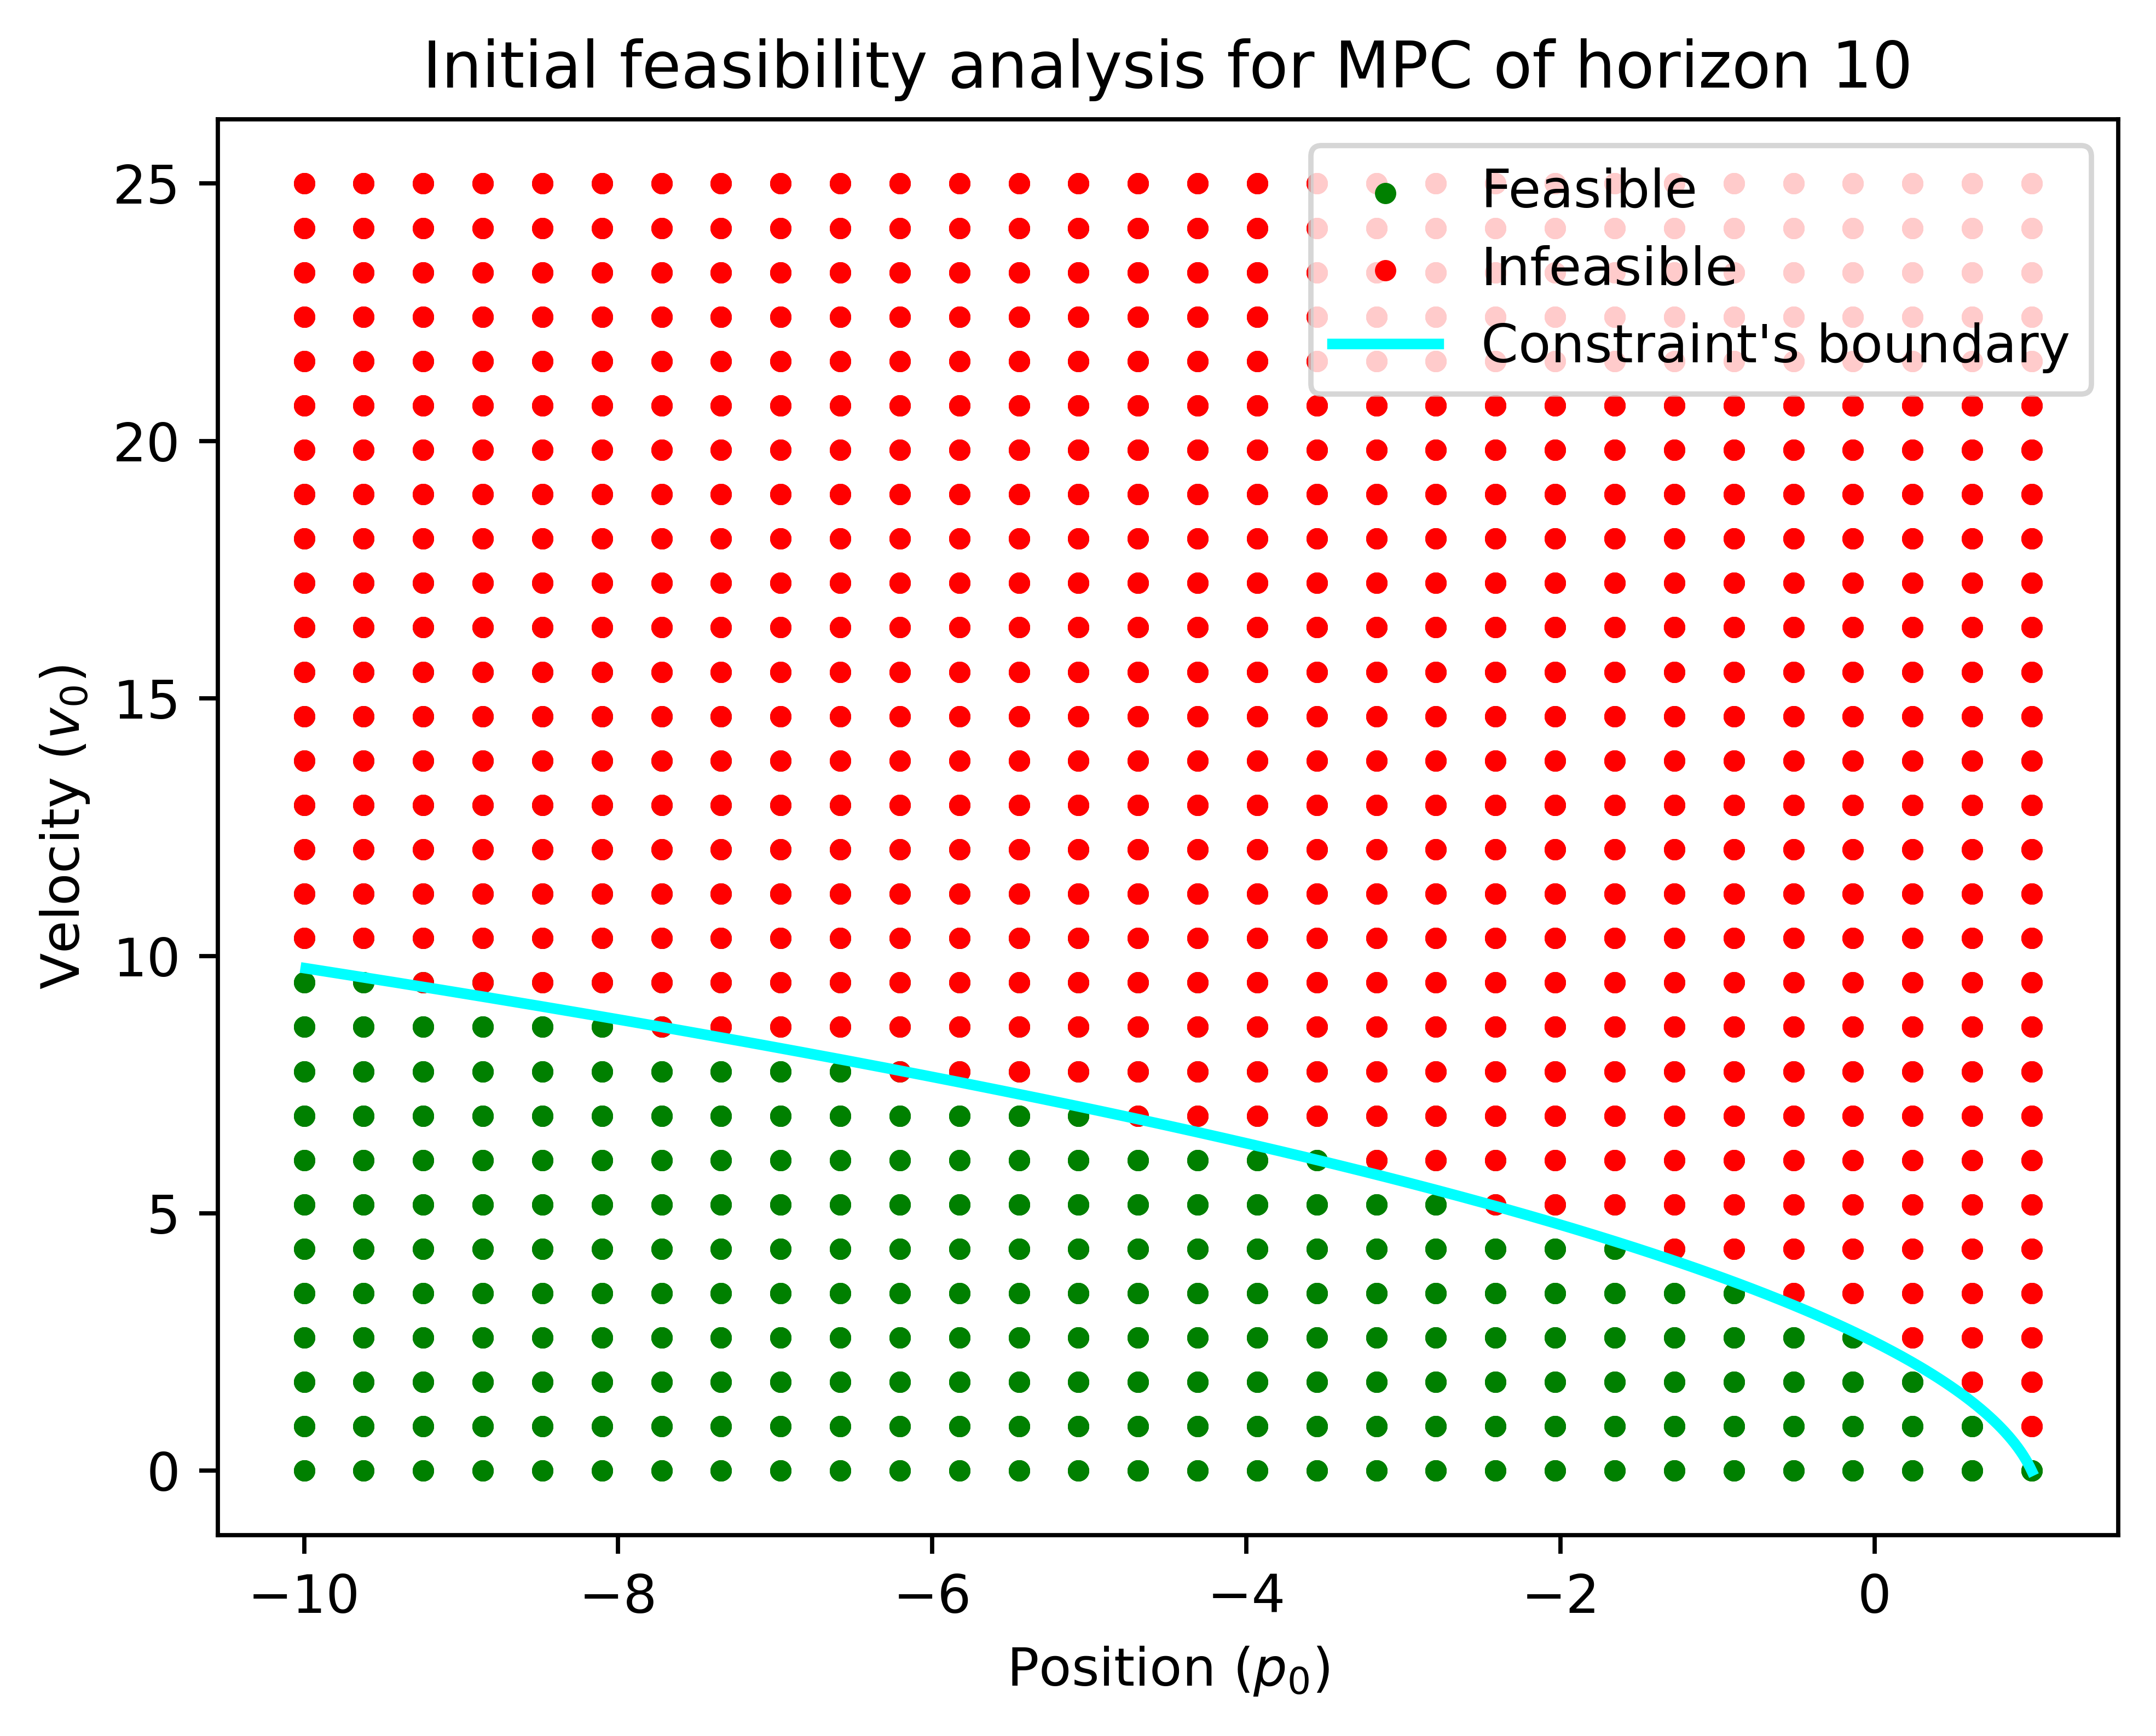
\includegraphics[width=\textwidth]{images/Assignment_24_N10.png}
        \caption{$N$ = 10}
        \label{fig:assignment2_4_3}
    \end{minipage}
\end{figure}



\newpage
\section{MPC theory: terminal ingredients}
During the sessions, we have computed polyhedral invariant sets to use 
for the terminal ingredients in our MPC controller. 
Alternatively, we can use ellipsoidal sets. 
The goal of this assignment is to compute such sets in a few different ways 
and compare them with the invariant sets we've computed during 
the session.

\begin{assignment} \label{sess3:assign-lqr}
	Let $K, P$ denote the optimal, infinite-horizon LQR gain and the solution of 
	the discrete-time Riccati equation, respectively. As shown in the lectures, 
	any level set
	\[ 
		\lev_{\alpha} V_{\infty} = \{x \mid V_{\infty}(x) = x^\top P x \leq \alpha\}
	\]
	is a positive invariant set for the system under the policy $u = Kx$. However, 
	not all states $x \in \lev_{\alpha} V_{\infty}$ necessarily satisfy the state and input constraints. 

	Write down the expression for the largest value of $\alpha$ 
	such that
	\[ 
	\begin{cases}
		x \in X \\
		Kx \in U  
	\end{cases} \quad \forall x \in \lev_{\alpha} V_{\infty},
	\]
	where $X = \{x \in \R^n \mid H_x x \leq h_x\}$ and $U = \{u \in \R^m \mid H_u u \leq h_u \}$ are 
	the (polyhedral) sets of feasible states and inputs, respectively.

	\textbf{Hint.} The notion of a support function might be of use.
\end{assignment}
\begin{flushleft}
	Given $ X_f = \left\{ x \in \R^n \mid x^T P x \le \alpha \right\} $, pick $ P \in S^{n_x}_{+} $ and $\alpha > 0$
	such that $ X_f $ is positive invariant for $ x^+ = A_k x $ and $ X_f \subseteq X_k $.
	We will pick $ P = P_f $: $ x_f = \left\{ x \in \R^{n_x} \mid V_f(x) \le \alpha \right\} $ since $ V_f $ is a Lyapunov function: $V(x^+) \le V_f(x) - \alpha(\| x \|) $.
	Now we should find the largest $\alpha$ such that $ X_f $ is as large as possible but still within $ X_k $, $ X_f \subseteq X_k $.
	\[
	\begin{aligned}
		X_k &= \left\{ x \in X \mid K_x \in U \right\} \\
			&= \left\{ x \in R^{n_x} \mid H_x x \le h_x, H_u K x \le h_u \right\} \\
			&= \left\{ x \in R^{n_x} \mid \begin{bmatrix}
				H_x \\
				H_u K 
			\end{bmatrix} x \le
			\begin{bmatrix}
				h_x \\
				h_u
			\end{bmatrix} \right\}
	\end{aligned} 
	\]
	Our objective is therefore to find the largest $\alpha$:
	\[ 
	\begin{aligned}
		\alpha &= \max \left\{ \alpha \mid X_f(\alpha) \subseteq X_k \right\} \\
			&= \max \left\{ h_i^T x \le g_i \mid x \in X_f(\alpha) \right\}
	\end{aligned}
	\]
	which, recalling that $ X_f(\alpha) \subseteq X_k = \left\{ x \mid h_i^T x \le g_i, \quad i = 1, \dots, m \right\} $ and implementing the support function $ \sigma_{X_f(\alpha)}(h_i) \le g_i$, can be written as:
	\[ 
		\max \left\{ h_i^T x \mid x^T P x \le \alpha \right\}
	\]
	Therefore, the lagrange function is:
	\[
		\mathcal{L}(x, \mu) = - h_i^T x + \mu g(x) = - h_i^T x + \mu (x^T P x - \alpha)
	\]
	Setting the gradient to zero, we obtain:
	\[ 
		\frac{\partial \mathcal{L}(x, \mu)}{\partial x} = - h_i + 2 \mu P x = 0 \implies x(\mu) = \frac{1}{2 \mu} P^{-1} h_i 
	\]
	Substituting $ x(\mu) $ back into the lagrange function, we obtain the dual function:
	\[
	\begin{aligned}
		q(\mu) = \mathcal{L}(x(\mu), \mu) &= - \frac{1}{2 \mu} h_i^T P^{-1} h_i - \mu \Bigg( \frac{1}{(2 \mu)^2} h_i^T P^{-1} P P^{-1} h_i - \alpha \Bigg) \\
			&= - \frac{1}{2 \mu} h_i^T P^{-1} h_i + \frac{1}{4 \mu} h_i^T P^{-1} h_i - \mu \alpha \\
			&= - \frac{1}{4 \mu} h_i^T P^{-1} h_i - \mu \alpha
	\end{aligned}
	\]	
	Solving the dual problem leads to:
	\[
		\dot{q}(\mu) = \frac{1}{4 \mu^2} h_i^T P^{-1} h_i - \alpha = 0 \implies \mu^* = \sqrt{\frac{1}{4 \alpha} h_i^T P^{-1} h_i}
	\]
	Finally the largest value of $\alpha$ can be obtained by solving:
	\[ 
		\max \left\{ \alpha \mid \sqrt{ \alpha h_i^T P^{-1} h_i } \le g_i, \quad i = 1, \dots, m\right\}
	\]
	which gives: 
	\[ \alpha = \min \left\{ \frac{g_i}{h_i^T P^{-1} h_i}, \quad i = 1, \dots, m \right\} \]
\end{flushleft}



\begin{assignment}
	Plot the ellipsoidal set 
	(You can use the given \texttt{Ellipsoid} class we provide,
	together with the function \texttt{visualization.plot\_ellipsoid} for this)
	together with the polyhedral set $\{ x \in \R^n \mid x \in X,\; Kx \in U \}$.
	Is the obtained ellipsoidal set a valid terminal set for the MPC problem? \\

	Alternatively, we can more directly encode the requirements for the invariant set and solve a convex optimization problem 
	to find it. 
	Let $E = \{ x \in \R^n \mid x^\top P x \leq 1 \}$ denote our candidate set, where 
	now $P$ is the positive definite shape matrix. 
	Let $K \in \R^{m \times n}$ furthermore be a candidate state feedback gain.
	Our goal is to determine 
	$P$ and $K$ to obtain the ``largest'' possible positive invariant set for 
	$x_{t+1} = A x_t + B u_t$ under the policy $u_t = K x_t$.
\end{assignment}
\begin{flushleft}
	The ellipsoidal set $E$, depicted in figure \ref{fig:assignment3_2} in yellow, is centered in $[0,0]$ and its size is defined by a shape matrix $P$, obtained from the Riccati recursion.
	Furthermore, by appropriately scaling the ellipsoid using the parameter $\alpha$, the largest possible ellipsoidal set that remains entirely within the polyhedral constraints is obtained. 
	The result is a maximized terminal set that touches precisely one boundary of the feasible polyhedral set, depicted in black, ensuring optimal usage of the allowable state space.
	
	This ellipsoid satisfies the necessary stability and feasibility requirements, since its entirely within $X_k$, additionally its positive invariance ensures 
	that it serves as a valid terminal set for the Model Predictive Control (MPC) probelm. 
\end{flushleft}
\begin{figure}[H]
    \centering
    \begin{minipage}{0.7\textwidth}
        \centering
        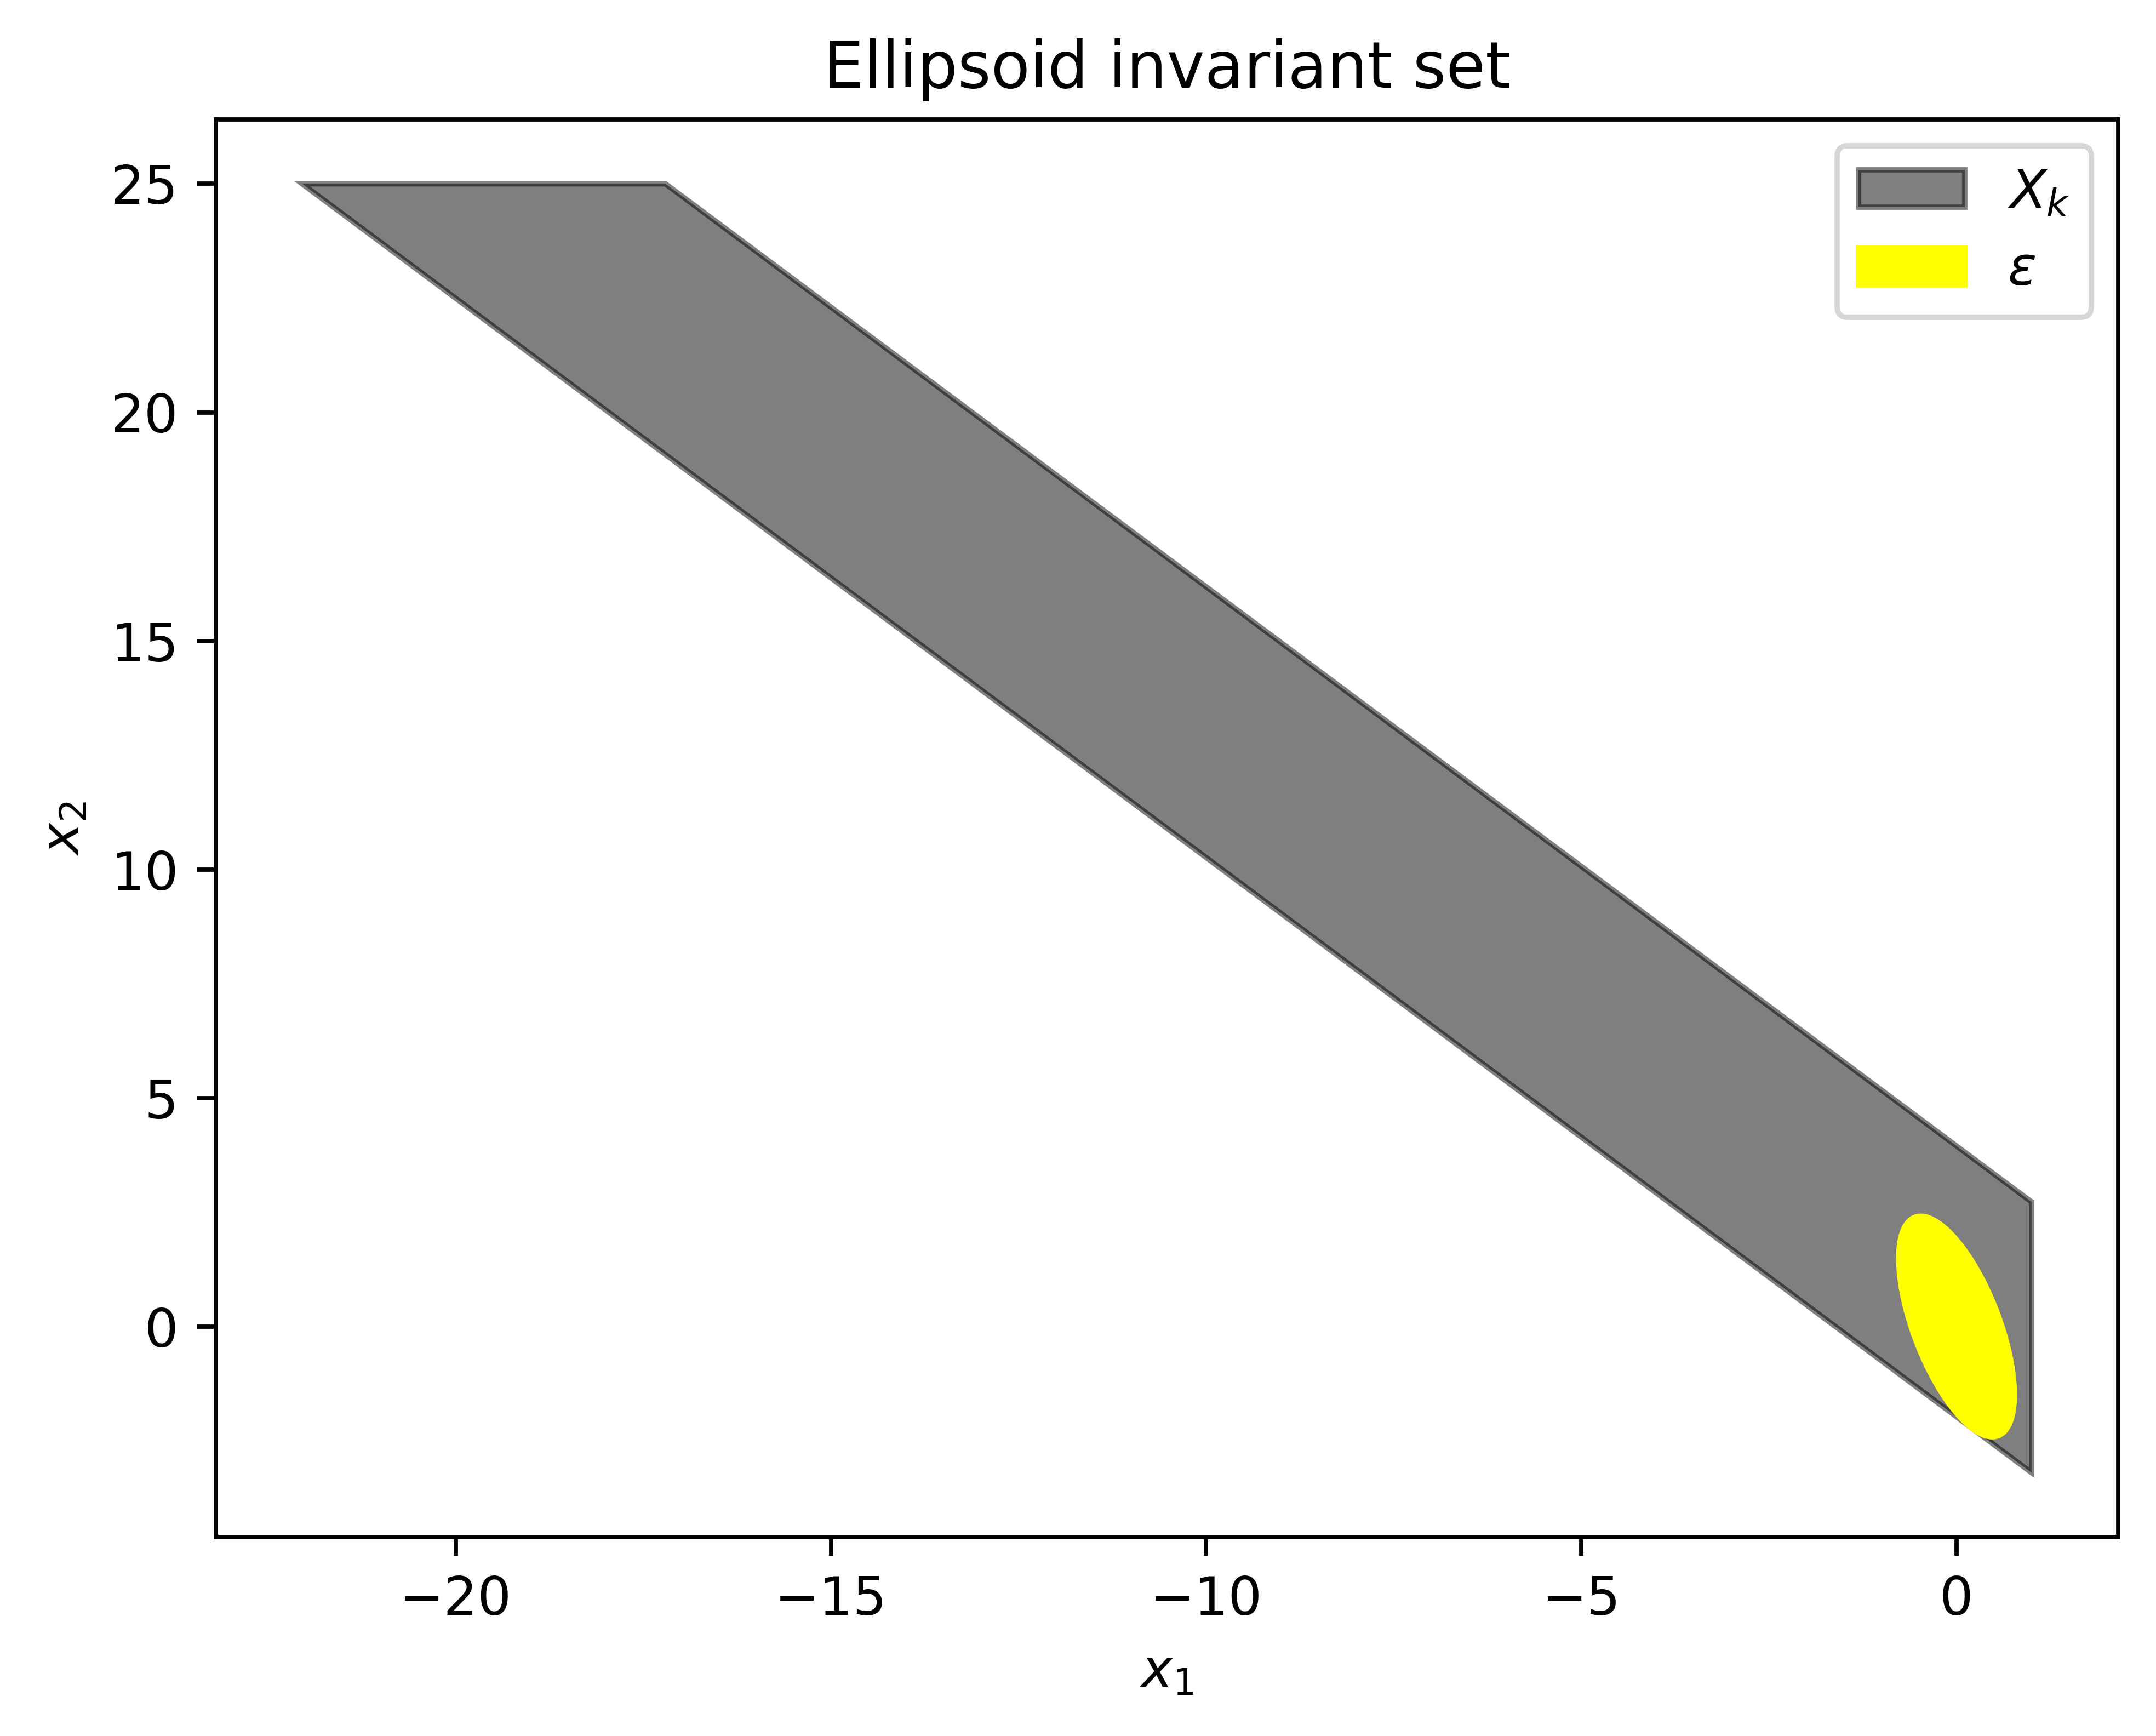
\includegraphics[width=\textwidth]{images/Assignment_32.png}
        \caption{Ellipsoidal set}
        \label{fig:assignment3_2}
    \end{minipage}
\end{figure}


\begin{assignment}
	Formulate a constraint on $P$ and $K$ that guarantees that 
	\[ 
		x^\top P x \leq 1 \implies x^\top(A + BK)^\top P (A + BK)x \leq 1  \quad \forall x \in \R
	\]
\end{assignment}
\begin{flushleft}
	To enforce positive invariance, if $x \in E$, then $x_{k+1} = (A + BK) x_k \in E$ too, we need:
\end{flushleft}
\begin{equation}
	x^\top(A + BK)^\top P (A + BK)x \preceq x^\top P x, \quad \forall x \in E
\end{equation}
Subtracting $x^\top P x$ from both sides, we obtain:
\begin{equation}
	x^\top\Big[ (A + BK)^\top P (A + BK) - P \Big] x \preceq 0
\end{equation}
This implies:
\begin{equation}
	(A + BK)^\top P (A + BK) - P \preceq 0
\end{equation}
The term $(A + BK)^\top P (A + BK) - P$ represents the "transformed" shape of the ellipsoid $E$ under the system dynamics, $u = Kx$. The constraint ensures that the transformed ellipsoid is contained within the original ellipsoid $E$, preserving invariance.



\begin{assignment}\label{sess3:c1}
	Show that the previous constraint can be written as the linear matrix inequality (LMI)
	\[ 
		\begin{bmatrix}
			S & (AS + BF)^\top \\ 
			AS + BF & S
		\end{bmatrix} \geq 0
	\]
	\textbf{Hint.} Doing this involves the following steps. 
	\begin{enumerate}
		\item multiply the inequality you obtained from the left and the right by $P^{-1}$
		\item Introduce the change of variables
			\begin{itemize}
			\item $S=P^{-1}$
			\item $F=KS$
			\end{itemize}
		\item Apply the \href{https://inst.eecs.berkeley.edu/~ee127/sp21/livebook/thm_schur_compl.html}{Schur complement lemma}.
	\end{enumerate}
\end{assignment}
\begin{flushleft}
	Given $P = P^\top$ by construction, we can multiply the inequality by $P^{-1}$ from the left and the right:
\end{flushleft}
\begin{equation}
	\begin{aligned}
		P^{-1} \Big[ (A + BK)^\top P (A + BK) - P \Big] P^{-1} &\preceq 0 \\  
		P^{-1} (A + BK)^\top P (A + BK) P^{-1} - P^{-1} &\preceq 0 \\
	\end{aligned}
\end{equation}
Let's introduce the change of variables:
\begin{equation}
	\begin{aligned}
		S = P^{-1} &\implies P = S^{-1}\\
		F = KS &\implies K = FS^{-1}
	\end{aligned}
\end{equation}
Therefore, we have that:
\begin{equation}
	\begin{aligned}
		S \Big[A + B ( F S^{-1}) \Big]^\top S^{-1} \Big[A + B ( F S^{-1} ) \Big] S - S &\preceq 0 \\
		S \Big[A^\top + S^{-1} F^\top B^\top \Big] S^{-1} \Big[A + B ( F S^{-1} ) \Big] S - S &\preceq 0 \\
		\Big[A S + B F \Big]^\top S^{-1} \Big[A S + B F \Big] - S &\preceq 0 \\
		S - \Big[A S + B F \Big]^\top S^{-1} \Big[A S + B F \Big] &\succeq 0
	\end{aligned}
\end{equation}
Finally, applying the Schur complement lemma, we obtain the desired LMI:
\begin{equation}
	\begin{aligned}
		\begin{bmatrix}
			S & (AS + BF)^\top \\ 
			AS + BF & S
		\end{bmatrix} &\succeq 0
	\end{aligned}
\end{equation}



\begin{assignment}\label{sess3:c2}
	Recall from the lectures that 
	\[ 
		E \subseteq \{x \in \R^n \mid Hx \leq g \} \iff \sigma_{E}(H_{i}) \leq g_i, \,\forall i = 1, \dots, p,
	\]
	where $\sigma_E$ denotes the support function of the ellipsoid $E$ and $H_i$ the $i$th row of $H$. 
	Use this fact to show that all states in our candidate invariant set $E$ satisfy the state constraints if and only if 
	\[ 
		H_{x,i}^\top S H_{x,i} \leq h_{x,i}^2, \quad i = 1, \dots, m_x,
	\]
	with $H_{x,i}$ the $i$th row of $H_x$ and $h_{x,i}$ the $i$th coordinate of $h_x$ (see \cref{sess3:assign-lqr})
	and $S = P^{-1}$ as before.

	\textbf{Hint.} An expression for the support function of an Ellipsoid is given in the 
	slides. (It's also a useful exercise to derive it yourself from the definition, but this is not part of the assignment) 
\end{assignment}
\begin{flushleft}
	Developing the definition of the ellipsoid $E$:
\end{flushleft}
\[ 
    E \subseteq \{x \in \mathbb{R}^n \mid Hx \leq g \} \equiv 
    \left\{ x \in \mathbb{R}^n \mid 
    \begin{bmatrix}
        H_x \\
        K^\top H_u
    \end{bmatrix} x \leq 
    \begin{bmatrix}
        h_x \\
        h_u
    \end{bmatrix} 
    \right\}
\]
The support function of the ellipsoid $E$ is given by:
\[ 
	\sigma_E(v) = \alpha^{1/2} \|P^{1/2} v\|_2
\] 
Therefore, knowing that $ P^{-1} = S $, we can write the support function as:
\begin{equation}
	\begin{aligned}
		\sigma_E(H_i) &= \alpha^{1/2} \|S^{1/2} H_i\|_2 \\
					  &= \alpha^{1/2} \Big[ \Big( S^{1/2} H_i \Big)^\top \Big( S^{1/2} H_i \Big) \Big]^{1/2} \\
					  &= \alpha^{1/2} \Big( H_i^\top S H_i \Big)^{1/2}
	\end{aligned}
\end{equation}
Since we are interested only in the states and $x^\top P x \leq 1 \implies \alpha = 1$:
\begin{equation}
		\sigma_E(H_{x,i}) = \Big( H_{x,i}^\top P H_{x,i} \Big)^{1/2} \leq g_{x,i} = h_{x,i} \implies \Big( H_{x,i}^\top S H_{x,i} \Big) \leq {h^2}_{x,i}, \quad \forall i = 1, \dots, m_x
\end{equation}



\begin{assignment}\label{sess3:c3}
	Similarly, show that $u = Kx$ satisfies the input constraints for all $x \in E$, 
	if and only if 
	\[ 
		h_{u,i}^2 - H_{u,i}^\top F P F^\top H_{u,i} \geq 0, \quad \forall i = 1, \dots, m_{u}.
	\]
	Use the Schur complement lemma to write this constraint as an LMI in $F$ and $S$.
\end{assignment}
\begin{flushleft}
	Developing the definition of the ellipsoid $E$:
\end{flushleft}
\[ 
    E \subseteq \{x \in \mathbb{R}^n \mid Hx \leq g \} \equiv 
    \left\{ x \in \mathbb{R}^n \mid 
    \begin{bmatrix}
        H_x \\
        K^\top H_u
    \end{bmatrix} x \leq 
    \begin{bmatrix}
        h_x \\
        h_u
    \end{bmatrix} 
    \right\}
\]
As previously seen, knowing that $ P^{-1} = S $, we can write the support function as:
\begin{equation}
	\sigma_E(H_i) = \alpha^{1/2} \Big( H_i^\top S H_i \Big)^{1/2}
\end{equation}
Since we are interested only in the inputs and knowing that $ K = F S^{-1} $:
\begin{equation}
	\begin{aligned}
		\sigma_E(K^\top H_{u,i}) &= \sigma_E(S^{-1} F^\top H_{u,i}) \\
								 &= \Big( H_{u,i}^\top F S^{-1} S S^{-1} F^\top H_{u,i} \Big)^{1/2} \leq g_{u,i} = h_{u,i} \\
								 &= \Big( H_{u,i}^\top F S^{-1} F^\top H_{x,i} \Big) \leq {h^2}_{u,i} \\
								 &\implies h_{u,i}^2 - H_{u,i}^\top F P F^\top H_{u,i} \succeq 0, \quad \forall i = 1, \dots, m_{u}
	\end{aligned}
\end{equation}
Applying the Schur complement lemma, we obtain the desired LMI:
\begin{equation}
	\begin{aligned}
		\begin{bmatrix}
			h_{u,i}^2 & H_{u,i}^\top F \\ 
			F^\top H_{u,i} & S
		\end{bmatrix} &\succeq 0
	\end{aligned}
\end{equation}



\begin{assignment}
	Since the volume of the ellipsoid is proportional to $\log \det P^{-1}$, we can now 
	compute the largest (in terms of volume) invariant set by maximizing $\log \det S$ subject 
	to the constraints in \cref{sess3:c1,sess3:c2,sess3:c3}. 
	
	Implement this problem using \texttt{cvxpy} and plot the resulting ellipsoid (using the given utility code as before.)
\end{assignment}
\begin{flushleft}
	The largest invariant set, represented by the ellipsoid, has been computed by: 
	\begin{equation}
		\begin{aligned}
			& \underset{S}{\text{minimize}}
			& & -\log \det S \\
			& \text{subject to}
			& & \text{constraints in \cref{sess3:c1,sess3:c2,sess3:c3}}
		\end{aligned}
	\end{equation} 
	The constraints, elaborated in the previous sections of this assignment, have been formulated as LMI. The resulting ellipsoid is shown in the figure \ref{fig:assignment3_7}. 
	Notably, this ellipsoid touches two boundaries of the polyhedral set, demonstrating that it has been scaled to its maximum possible size while remaining entirely within the feasible region. 
	This ensures the ellipsoid fully satisfies the constraints, serving as the largest admissible invariant set for the MPC problem.
\end{flushleft}
\begin{figure}[H]
    \centering
    \begin{minipage}{0.7\textwidth}
        \centering
        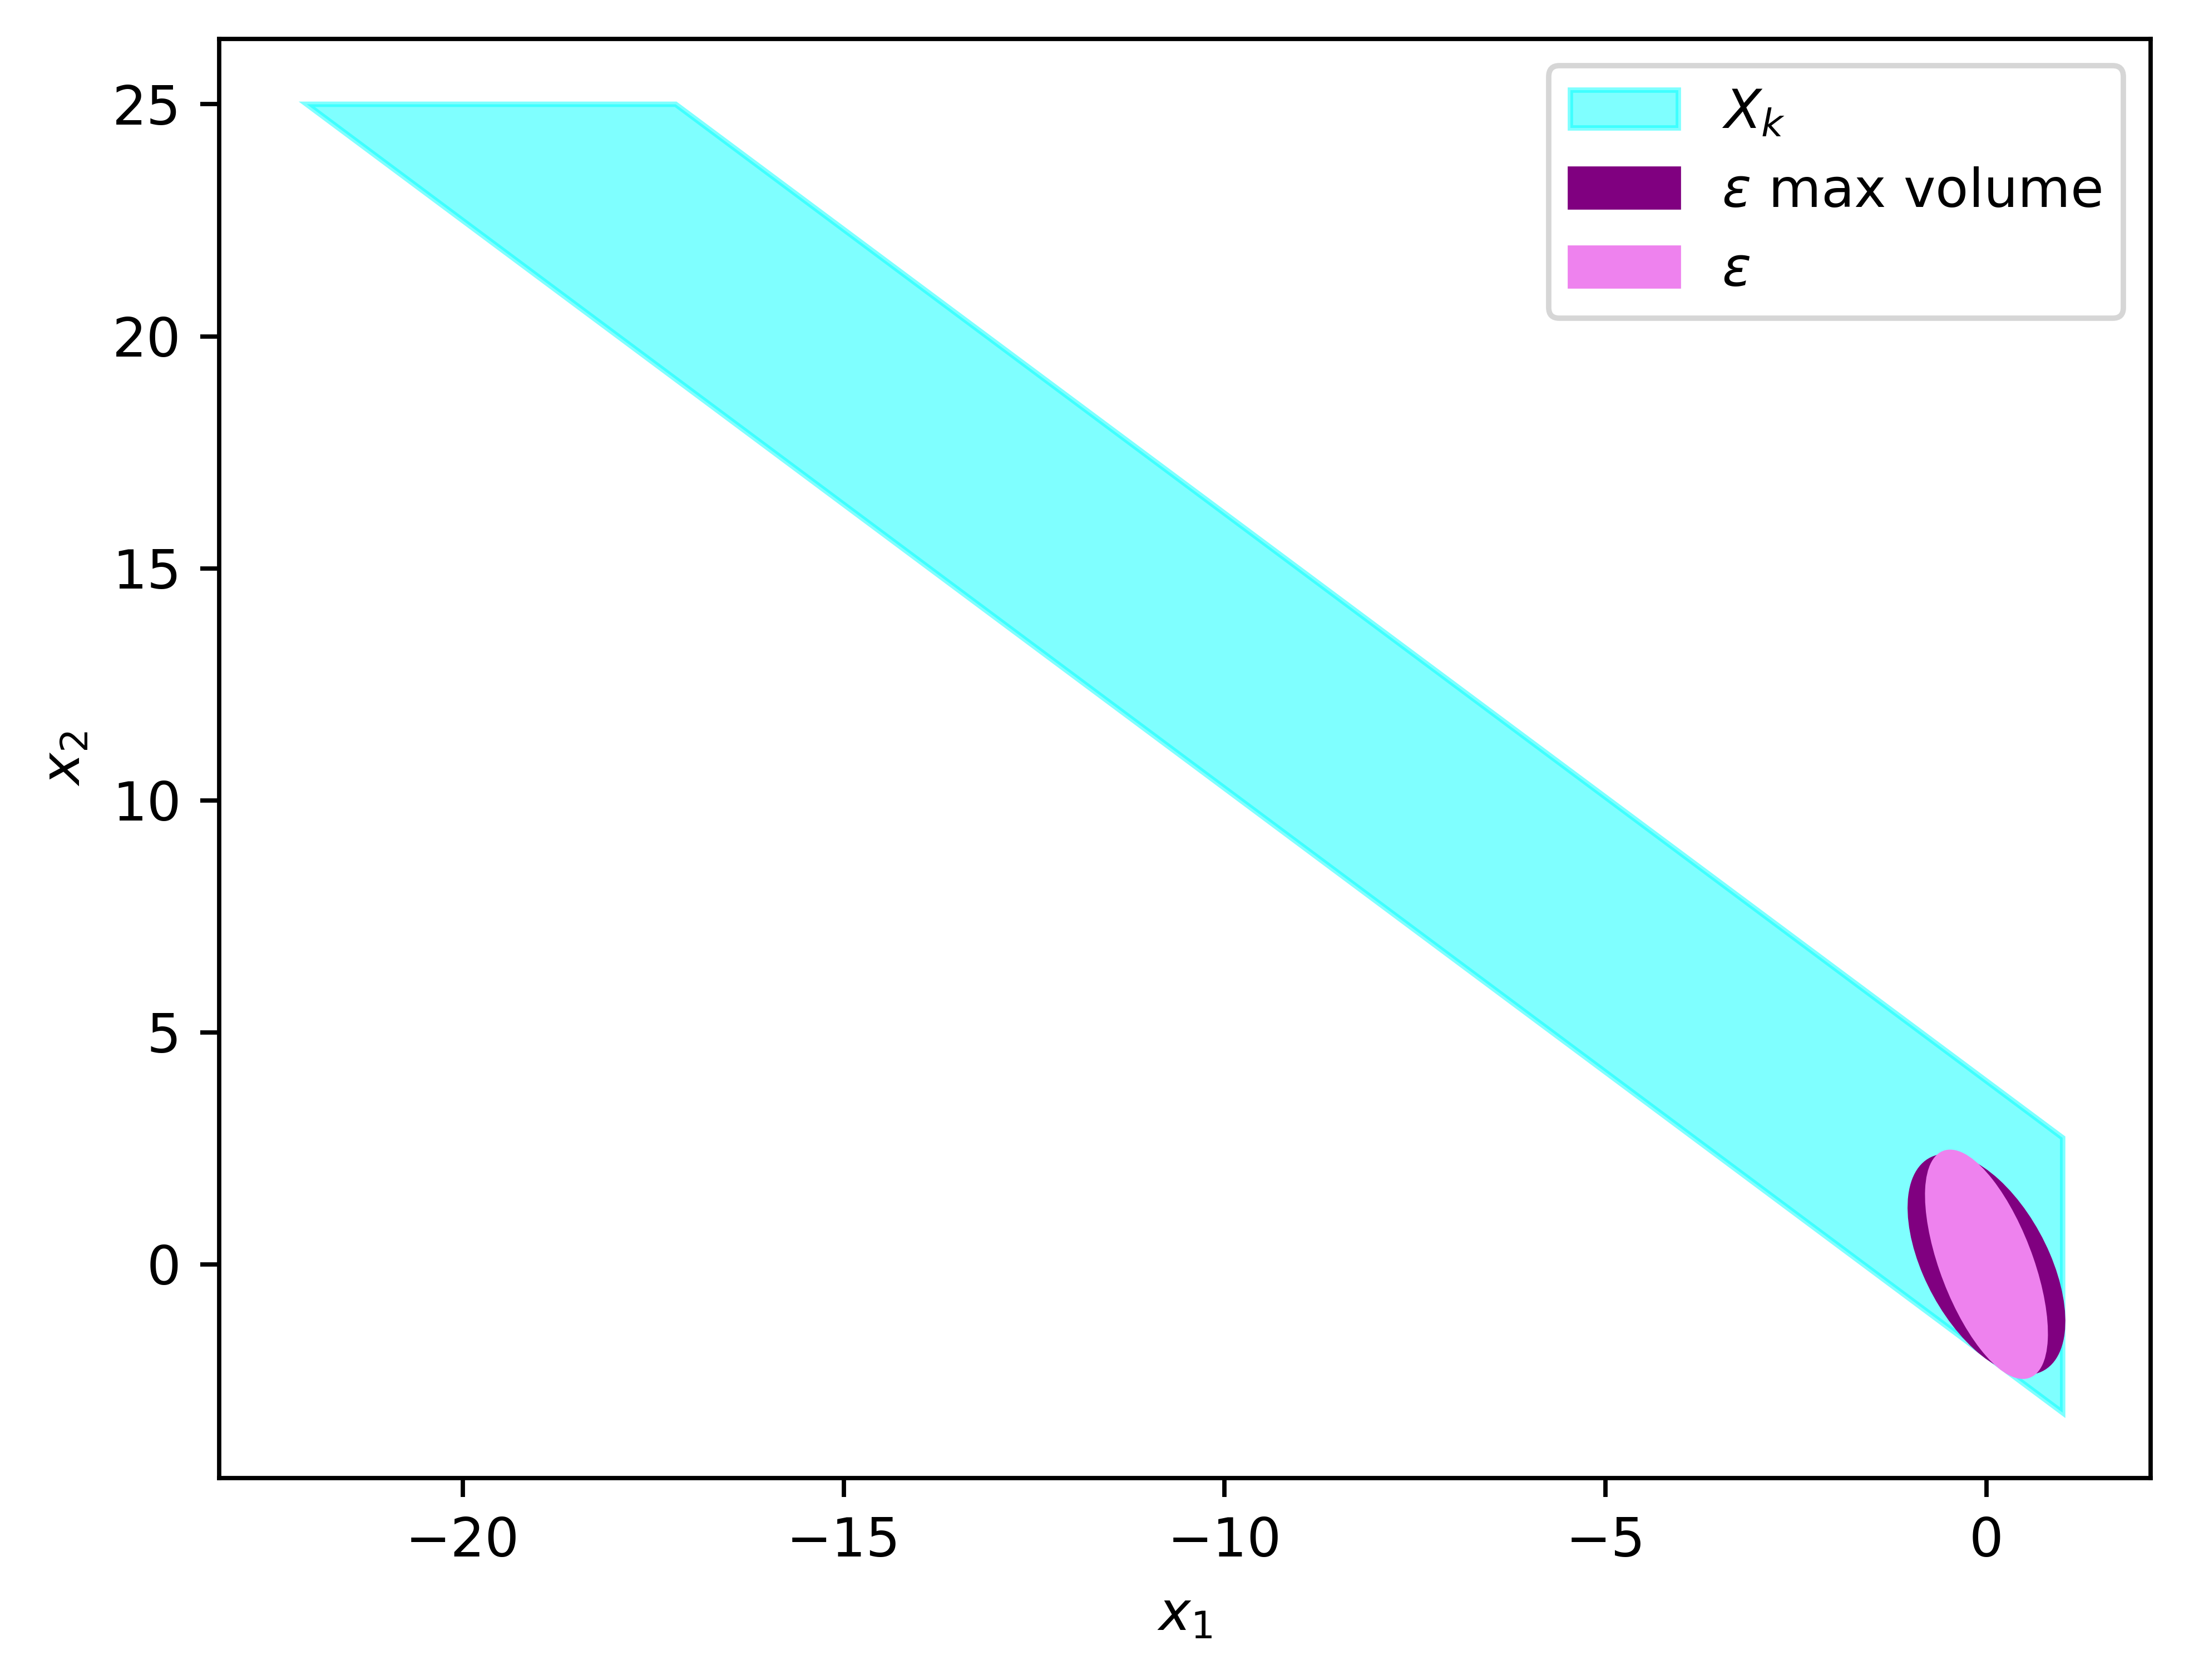
\includegraphics[width=\textwidth]{images/Assignment_37.png}
        \caption{Ellipsoidal sets}
        \label{fig:assignment3_7}
    \end{minipage}
\end{figure}




\newpage
\section{Nonlinear MPC}

We revisit the autonomous parking task but in a slightly more challenging situation. 
Suppose that there is a vehicle in the adjacent parking spot. 

\begin{figure}[ht!]
    \centering 
    \begin{tikzpicture}
        \tikzset{point/.style={circle, fill, inner sep=1pt}}
        \newlength{\pwid}
        \setlength{\pwid}{1cm}
        \newlength{\phei}
        \setlength{\phei}{0.48cm}
        \newlength{\cw}  % Car width 
        \newlength{\ch}  % Car height 
        \setlength{\cw}{0.8cm}
        \setlength{\ch}{0.4cm}
        
        \fill[gray!80!cyan] (-4\pwid, 1.5\phei) rectangle (4\pwid, -3\phei);
        \fill[black!70!cyan] (-4\pwid, 0.5\phei) rectangle (4\pwid, -3\phei); 
        \foreach\i in {-2,-1,...,2}{
            \begin{scope}[xshift=\i\pwid]
            \draw[very thick, white] (-0.5\pwid, -0.5\phei) rectangle (0.5\pwid, 0.5\phei);
            \end{scope}
        }
        \colorlet{carcol}{blue!50!cyan}
		\colorlet{obstaclecol}{red!80!black}
        \node[point, label=left:{\color{cyan}\textbf{Goal}}, color=cyan] {};
        \fill[carcol, rounded corners] (1.3\pwid-0.5\cw, -1.2\phei-0.5\ch) rectangle ++(\cw,\ch) coordinate[midway] (carcenter);
        \draw[->, >=stealth, thick, carcol] ($(carcenter)-(0.5\cw,0)$) to[in=0,out=180] (0,0); 
        \node[text=white] at (carcenter){car};
		
		\fill[obstaclecol, rounded corners] (1\pwid-0.5\cw, -0.5\ch) rectangle ++(\cw,\ch) coordinate[midway] (obscenter);
		\node[text=white] at (obscenter){obs};

    \end{tikzpicture}
    \caption{Autonomous parking task with obstacle}
    \label{fig:task}
\end{figure}

Naturally, the vehicle can in no circumstance be allowed to collide with the stationary obstacle. 
The goal of this assignment is to modify the MPC formulation from the exercise session to include collision avoidance constraints. 

One way of formulating the collision avoidance constraint is to cover each vehicle with a single row of circles as illustrated in  
\cref{fig:circles}. 
Here, $d$ denotes the horizontal distance between the center of each 
circle and its intersection with the rectangle, $r$ denotes the 
radius of the circles, $l$ is the length of the vehicle and $w$ is the width of the vehicle.

\begin{figure}[ht!]
	\centering
	\foreach \i in {2,3,5}{
	\begin{minipage}{0.3\textwidth}
	   \includegraphics[width=\textwidth]{figures/covering_circles\i.pdf}
	\end{minipage}
	}
	\caption{Vehicle covering with 2, 3 and 5 circles respectively.}
	\label{fig:circles}
\end{figure}


\newcommand{\nc}{n_{\mathrm{c}}}
\begin{assignment}
	Let $\nc$ denote the number of circles used to cover the vehicle. 
	Based on the figure, derive an expression 
	for the \textbf{centers} $c_i \in \R^2$, $i = 0, \dots, \nc-1$ 
	and the radius $r \in \R_+$ of the circles
	as a function of $l$, $w$ and $\nc$. 
	Assume that the origin lies in the center of the vehicle (i.e., the rectangle).
	
	Consider a vehicle of $l=4$ and $w=2$, and take $\nc=3$. 
	To verify your results, use \texttt{Circle} and \texttt{Rectangle} from \texttt{matplotlib.patches} 
	to plot it for this example.

	\textbf{Hint:} This task involves only basic geometry.
\end{assignment}
\begin{flushleft}
	Studying the figures, we can see derive an expression to compute d:
\end{flushleft}
\[
	d = \frac{l}{2 * nc} \quad \text{where } nc \text{ is the number of circles}
\]
Therefore the position of the center of the circles can be expressed as, taking into consideration the desired refernce frame:
\[
	c_i = \begin{bmatrix}
		- \frac{l}{2} + (1 + 2i)d \\
		0
	\end{bmatrix} \quad \text{where } c_i \text{ is the center of the i-th circle}
\]
Moroever, the radius of the circles, applying the Pitagora theorem, can be expressed as:
\[
	r = \sqrt{d^2 + \frac{w^2}{4}}
\]
Below, figure \ref{fig:assignment4_1}, a picture of the vehicle covered by 3 circles is shown.
\begin{figure}[H]
    \centering
    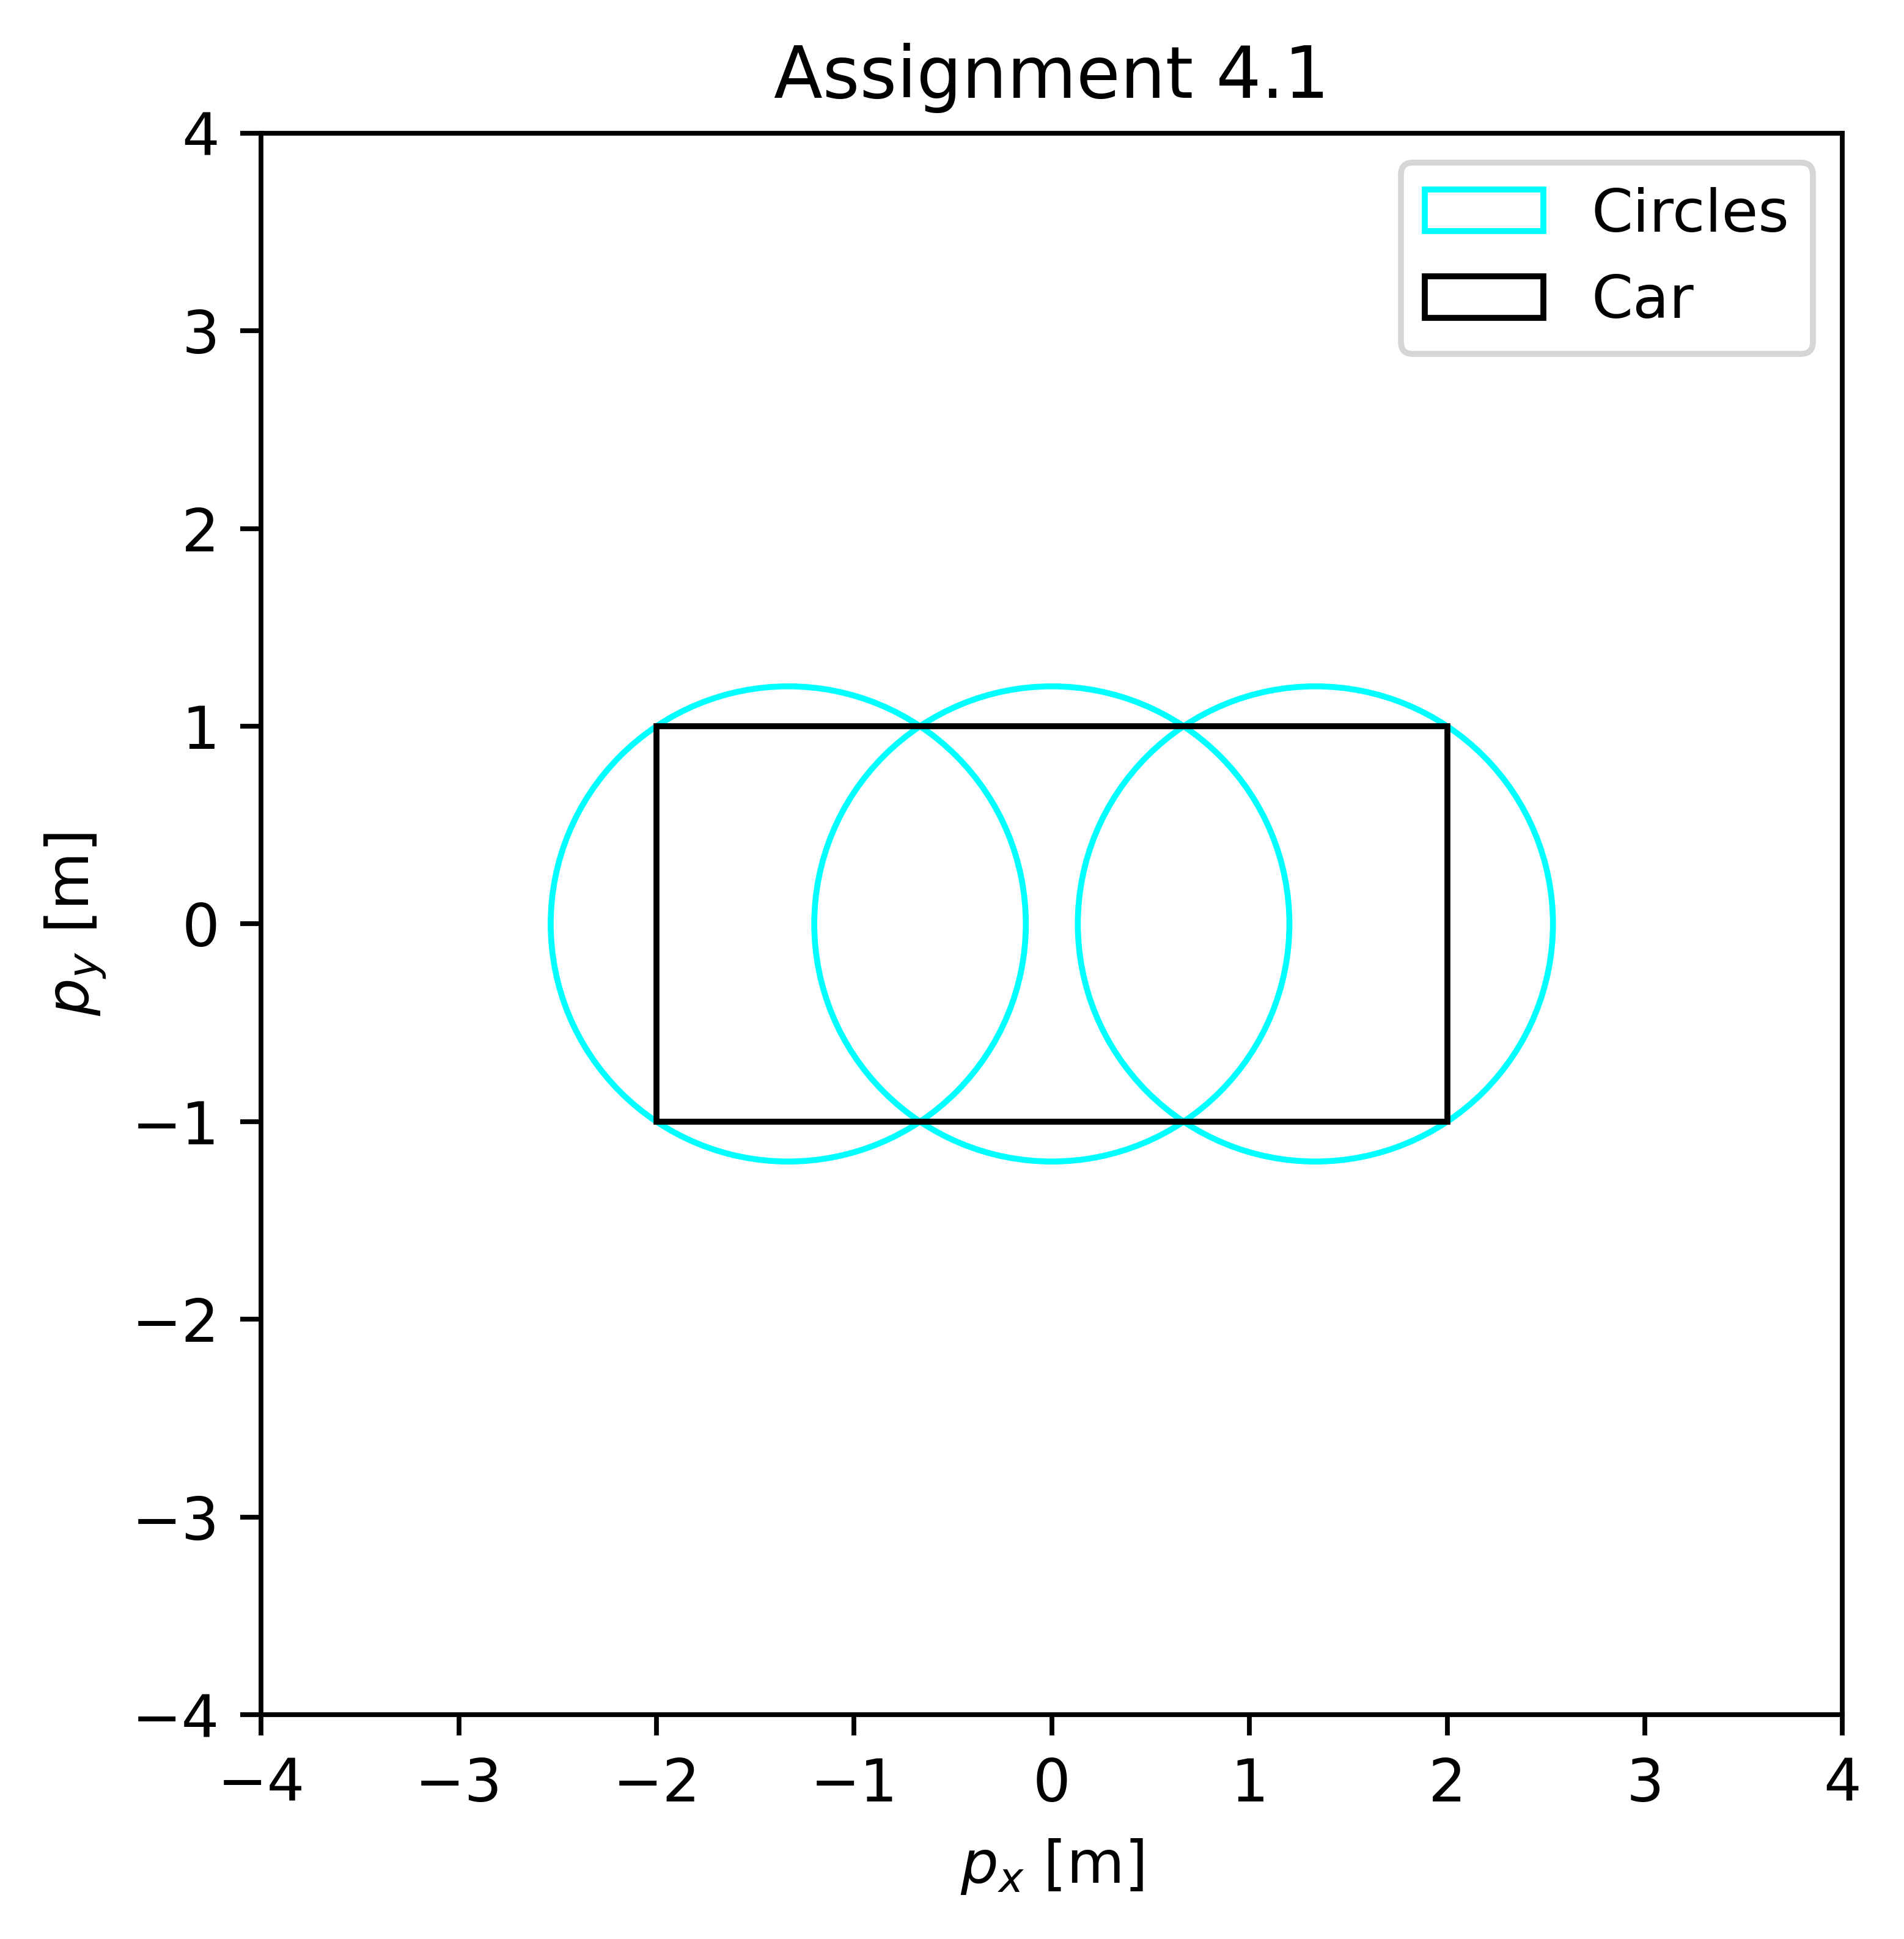
\includegraphics[width=0.7\textwidth]{images/Assignment_41.png}
    \caption{Vehicle covered by 3 circles}
    \label{fig:assignment4_1}
\end{figure}



\begin{assignment}
	Given that the current vehicle state is $x = (p_x, p_y, \psi, v)$, 
	express the center $\bar{c}$ of a circle in global coordinates, given that its local coordinates 
	(aligned with the vehicle, as in the previous exercise) are given by $c$.

	For a vehicle of length $l = 4$, width $w = 2$, with its center at $p = (2,2)$
	and heading angle $\psi = \tfrac{\pi}{4}$, use your result (combined with the previous assignment) to plot the 
	covering circles on this vehicle for $\nc = 3$.

	\textbf{Hint:} You can write your result in terms of the rotation matrix $R(\psi)$ defined by 
	the heading angle $\psi$. There is no need to work out everything into individual components.
\end{assignment}
\begin{flushleft}
	In order to go from local coordinates to global coordinates, we implement the rotation matrix $R(\psi)$:
\end{flushleft}
\[
	R(\psi) = \begin{bmatrix}
		\cos(\psi) & -\sin(\psi) \\
		\sin(\psi) & \cos(\psi)
	\end{bmatrix}
\]
And we sum to the circles' local coordinates obtained previously the global coordinates of the vehicle:
\[
	c_{i,global} = R c_{i,local} + p \quad \text{where } p \text{ is the position of the center of the car } 
	\begin{bmatrix}
		p_x \\ p_y
	\end{bmatrix}
\]
Below, figure \ref{fig:assignment4_2}, a picture of the vehicle having a yaw, $ \psi = \pi/4 $, positioned in $	p = [2, 2]^\top $ covered by 3 circles is shown.
\begin{figure}[H]
    \centering
    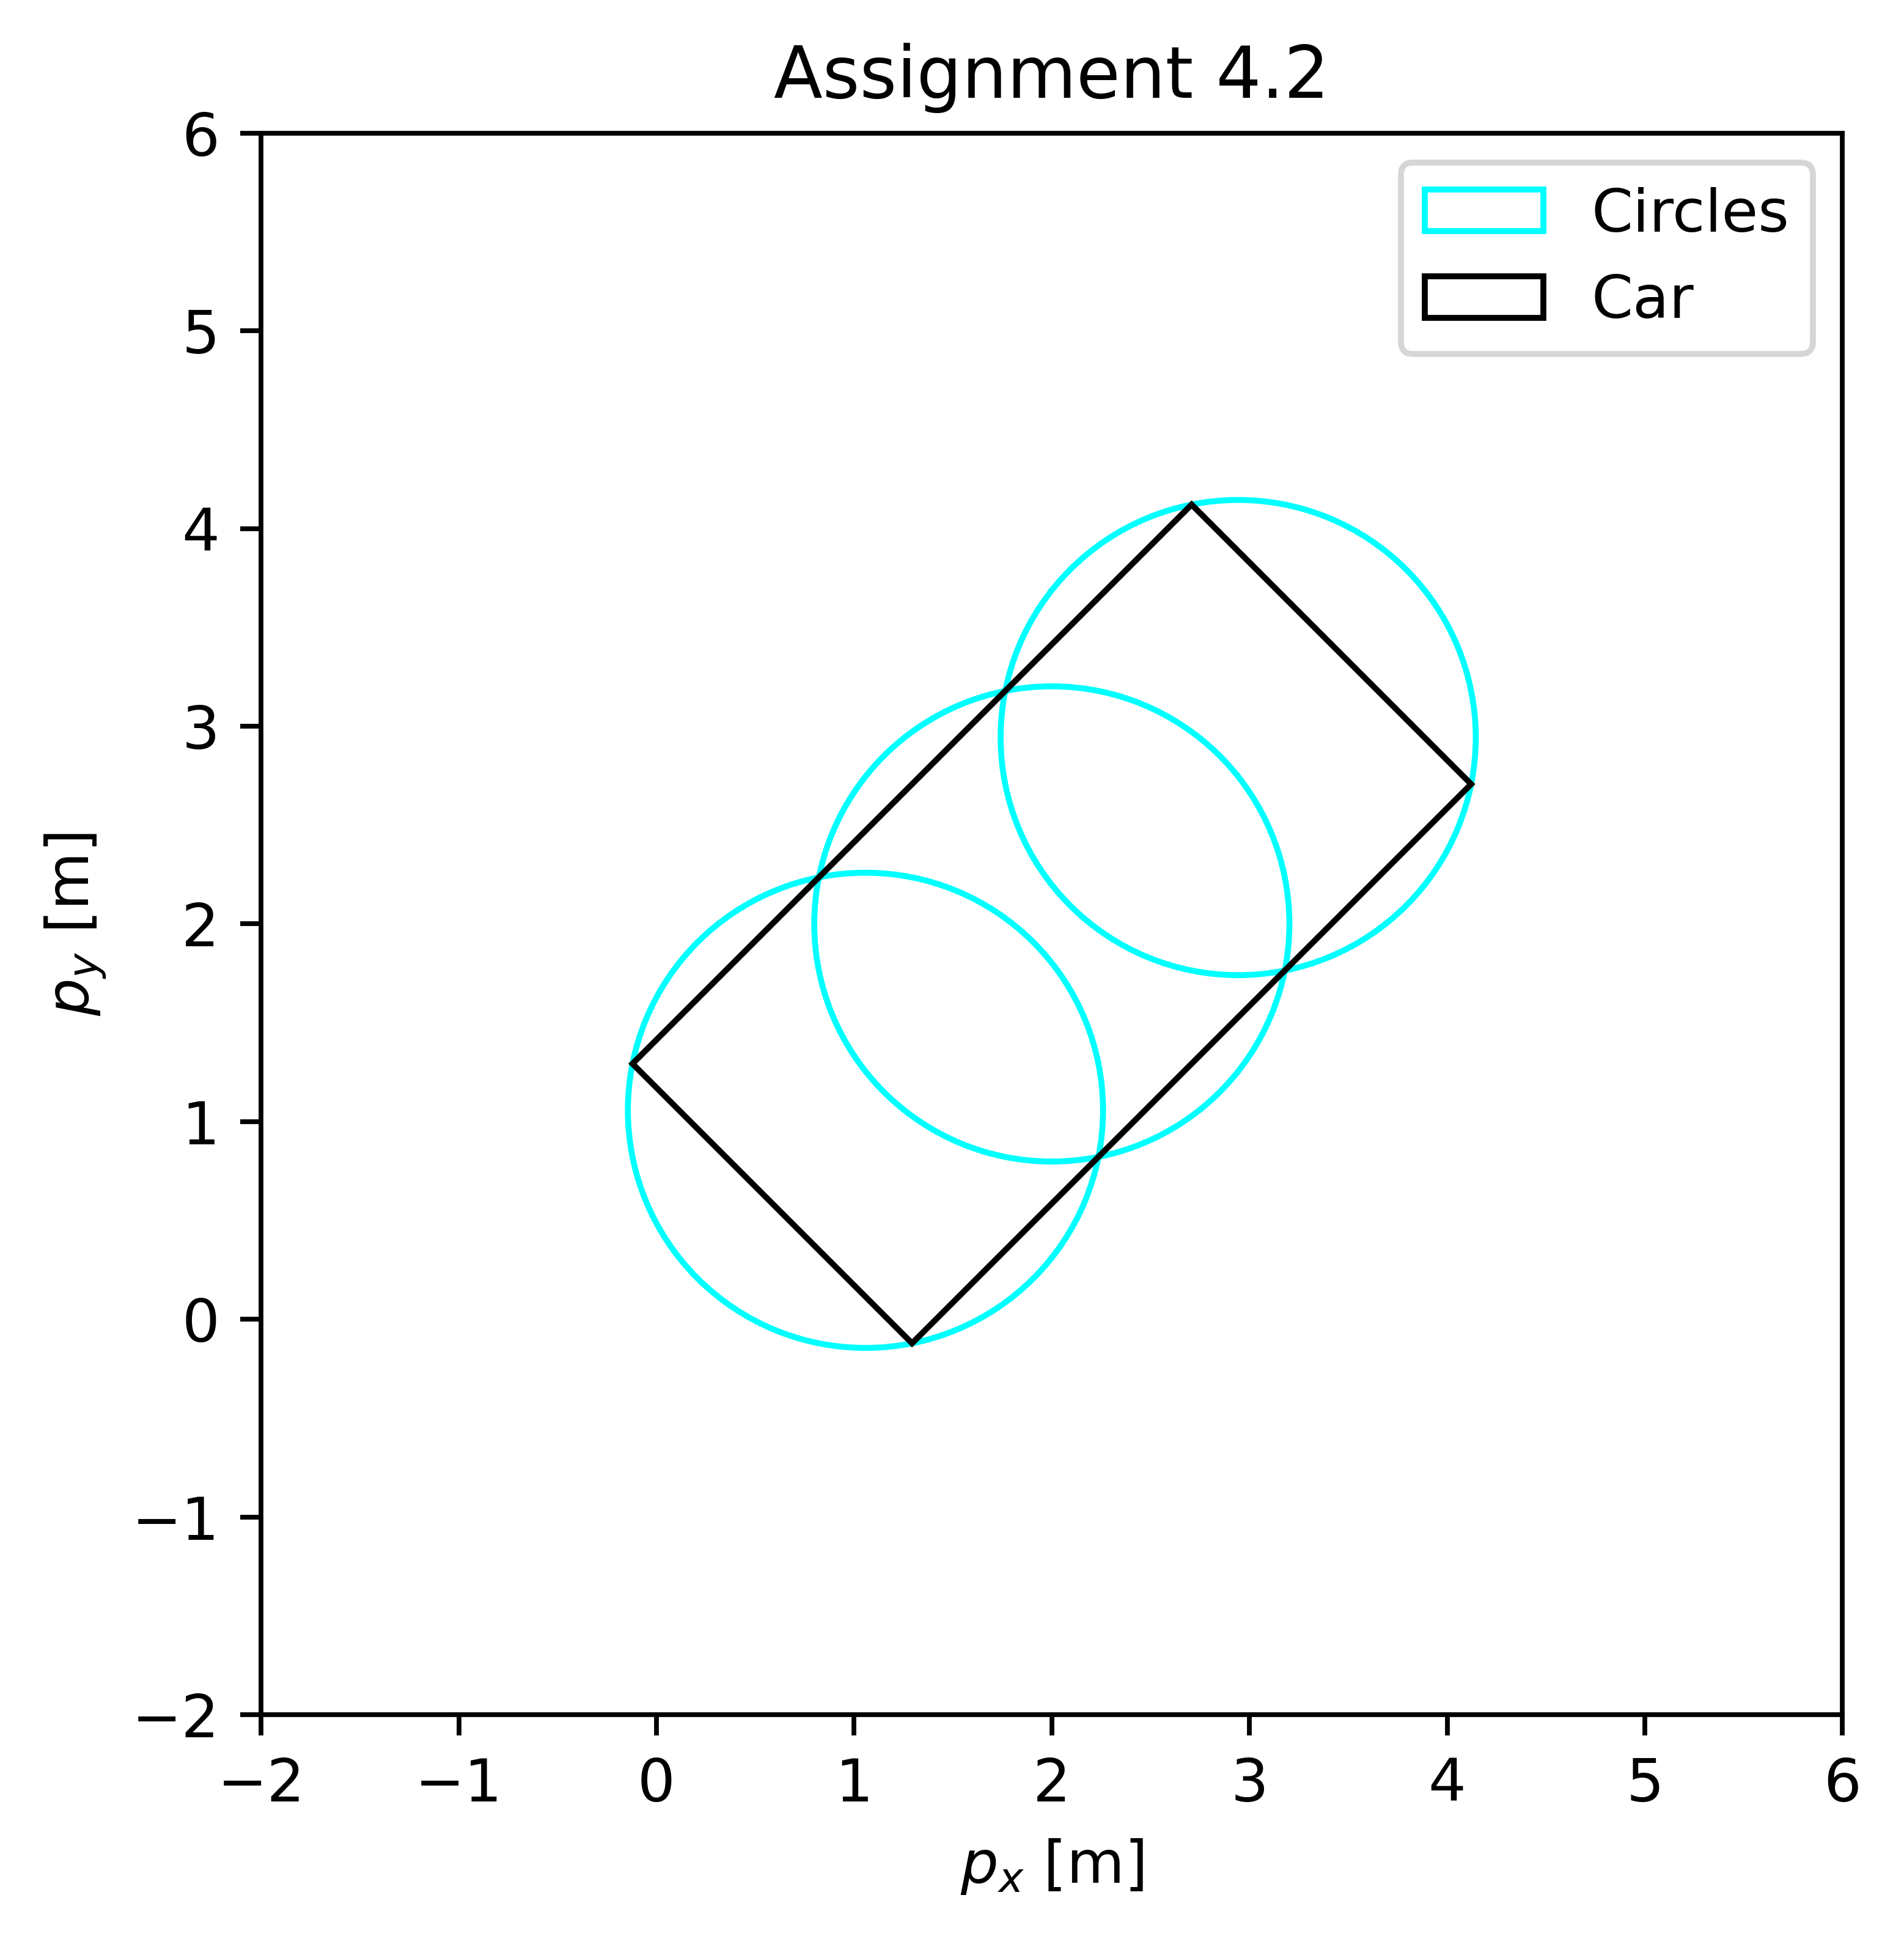
\includegraphics[width=0.7\textwidth]{images/Assignment_42.png}
    \caption{Vehicle global coordinates covered by 3 circles}
    \label{fig:assignment4_2}
\end{figure}



\begin{assignment}
	Given that the controlled vehicle is covered by circles with 
	centers $\bar{c}_i$ $i = 0, \dots, \nc-1$ (expressed in global coordinates) and
	radius $r$, and similarly the obstacle vehicle is covered by circles 
	with centers $\bar{c}_i'$ and radius $r'$. 
	Formulate a set of \textit{smooth} constraints 
	\[ 
		g(\bar{c}_i, \bar{c}_j) \leq 0
	\]
	on $\bar{c}_i$ and $\bar{c}_j'$, $i,j \in 0, \dots, \nc-1$.
	which -- when satisfied -- guarantees that the intersection between 
	the two vehicle rectangles is empty.

	Additionally, show whether this set of constraints is convex or not.

	\textbf{Hint:} Squaring can get rid of isolated points of non-smoothness.
\end{assignment}
\begin{flushleft}
	To guarantee that the intersection between the two vehicles is empty, using circles, we can formulate a constraint based on the distance between the centers of the circles and the sum of their radii. To guarantee the smoothness of the constraint, we can square both distances.
\end{flushleft}
The squared distance between the centers of the circles is:
\[
	d_{c}^2 = \|\bar{c}_i - \bar{c}_j'\|_2^2 = (\bar{c}_i - \bar{c}_j')^\top (\bar{c}_i - \bar{c}_j') \quad \forall i,j
\]
The squared sum of the radii is:
\[
	d_{r}^2 = (r + r')^2
\]
Therefore, the constraint can be formulated as:
\begin{equation}
	\begin{aligned}
		g(\bar{c}_i, \bar{c}_j') &= d_{r}^2 - d_{c}^2 \leq 0 \\
								 &= (r + r')^2 - (\bar{c}_i - \bar{c}_j')^\top (\bar{c}_i - \bar{c}_j') \leq 0
	\end{aligned}
\end{equation}
The euclidean norm squared is a convex function, the negative of a convex function is a concave function. Therefore, the constraint is concave because it is the sum between a concave function and a constant. 



\begin{assignment}
	Implement the constraint you derived into your MPC controller formulation.
	That is, enforce that 
	\[
		g(\bar{c}_i(x_t), \bar{c}_j') \leq 0, \quad \forall i,j \in \{0, \dots, \nc-1\}, \forall t \in 1, \dots, N. 
	\]
	where $\bar{c}_{i}(x_t)$ is the center (in global coordinates) of the $i$'th circle on the 
	controlled vehicle expressed as a function of its state at time step $t$,
	$\bar{c}_j'$ is the center (in global coordinates) of the $j$'th circle 
	on the obstacle vehicle and $g$ is the function you derived in the previous 
	exercise.

	Using the following settings, Simulate your MPC controller for 100 time steps in closed loop.
	You can use the MPC model dynamics for the simulation (no model mismatch):
	
	\begin{center}
	\begin{tabular}{cc}
		\toprule
		$x_0$ & $(0.3, -0.1, 0, 0)$ \\
		$N$   & 30 \\ 
		$\Ts$ & 0.08 \\ 
		Obstacle pos. & $(0.25, 0)$ (heading 0)\\
		\bottomrule
	\end{tabular}
	\end{center}
	
	Use \texttt{plot\_state\_trajectory} from \texttt{given.plotting} to 
	visualize the state trajectory, including the obstacle (simply pass the function a list with only one state, since it is stationary).
	Is the trajectory collision-free? 
	Does the car converge to a point that is entirely within the parking spot
	\footnote{
	defined in the code as a rectangle with dimensions \texttt{PARK\_DIMS=}$(0.25, 0.12)$
	}?

	Optionally, you can also generate an animation using \texttt{given.animation}, but this is 
	not a deliverable.
	(see the solution of the exercise session for some example code. You can use the argument \texttt{obstacle\_positions} to visualize the obstacle.)
\end{assignment}
\begin{flushleft}
	As can be seen in figure \ref{fig:assignment4_4}, using the default values for $Q$, $R$, and $N$, the trajectory is collision-free but the vehicle is not fully parked within the parking spot.
\end{flushleft}
\begin{figure}[H]
    \centering
    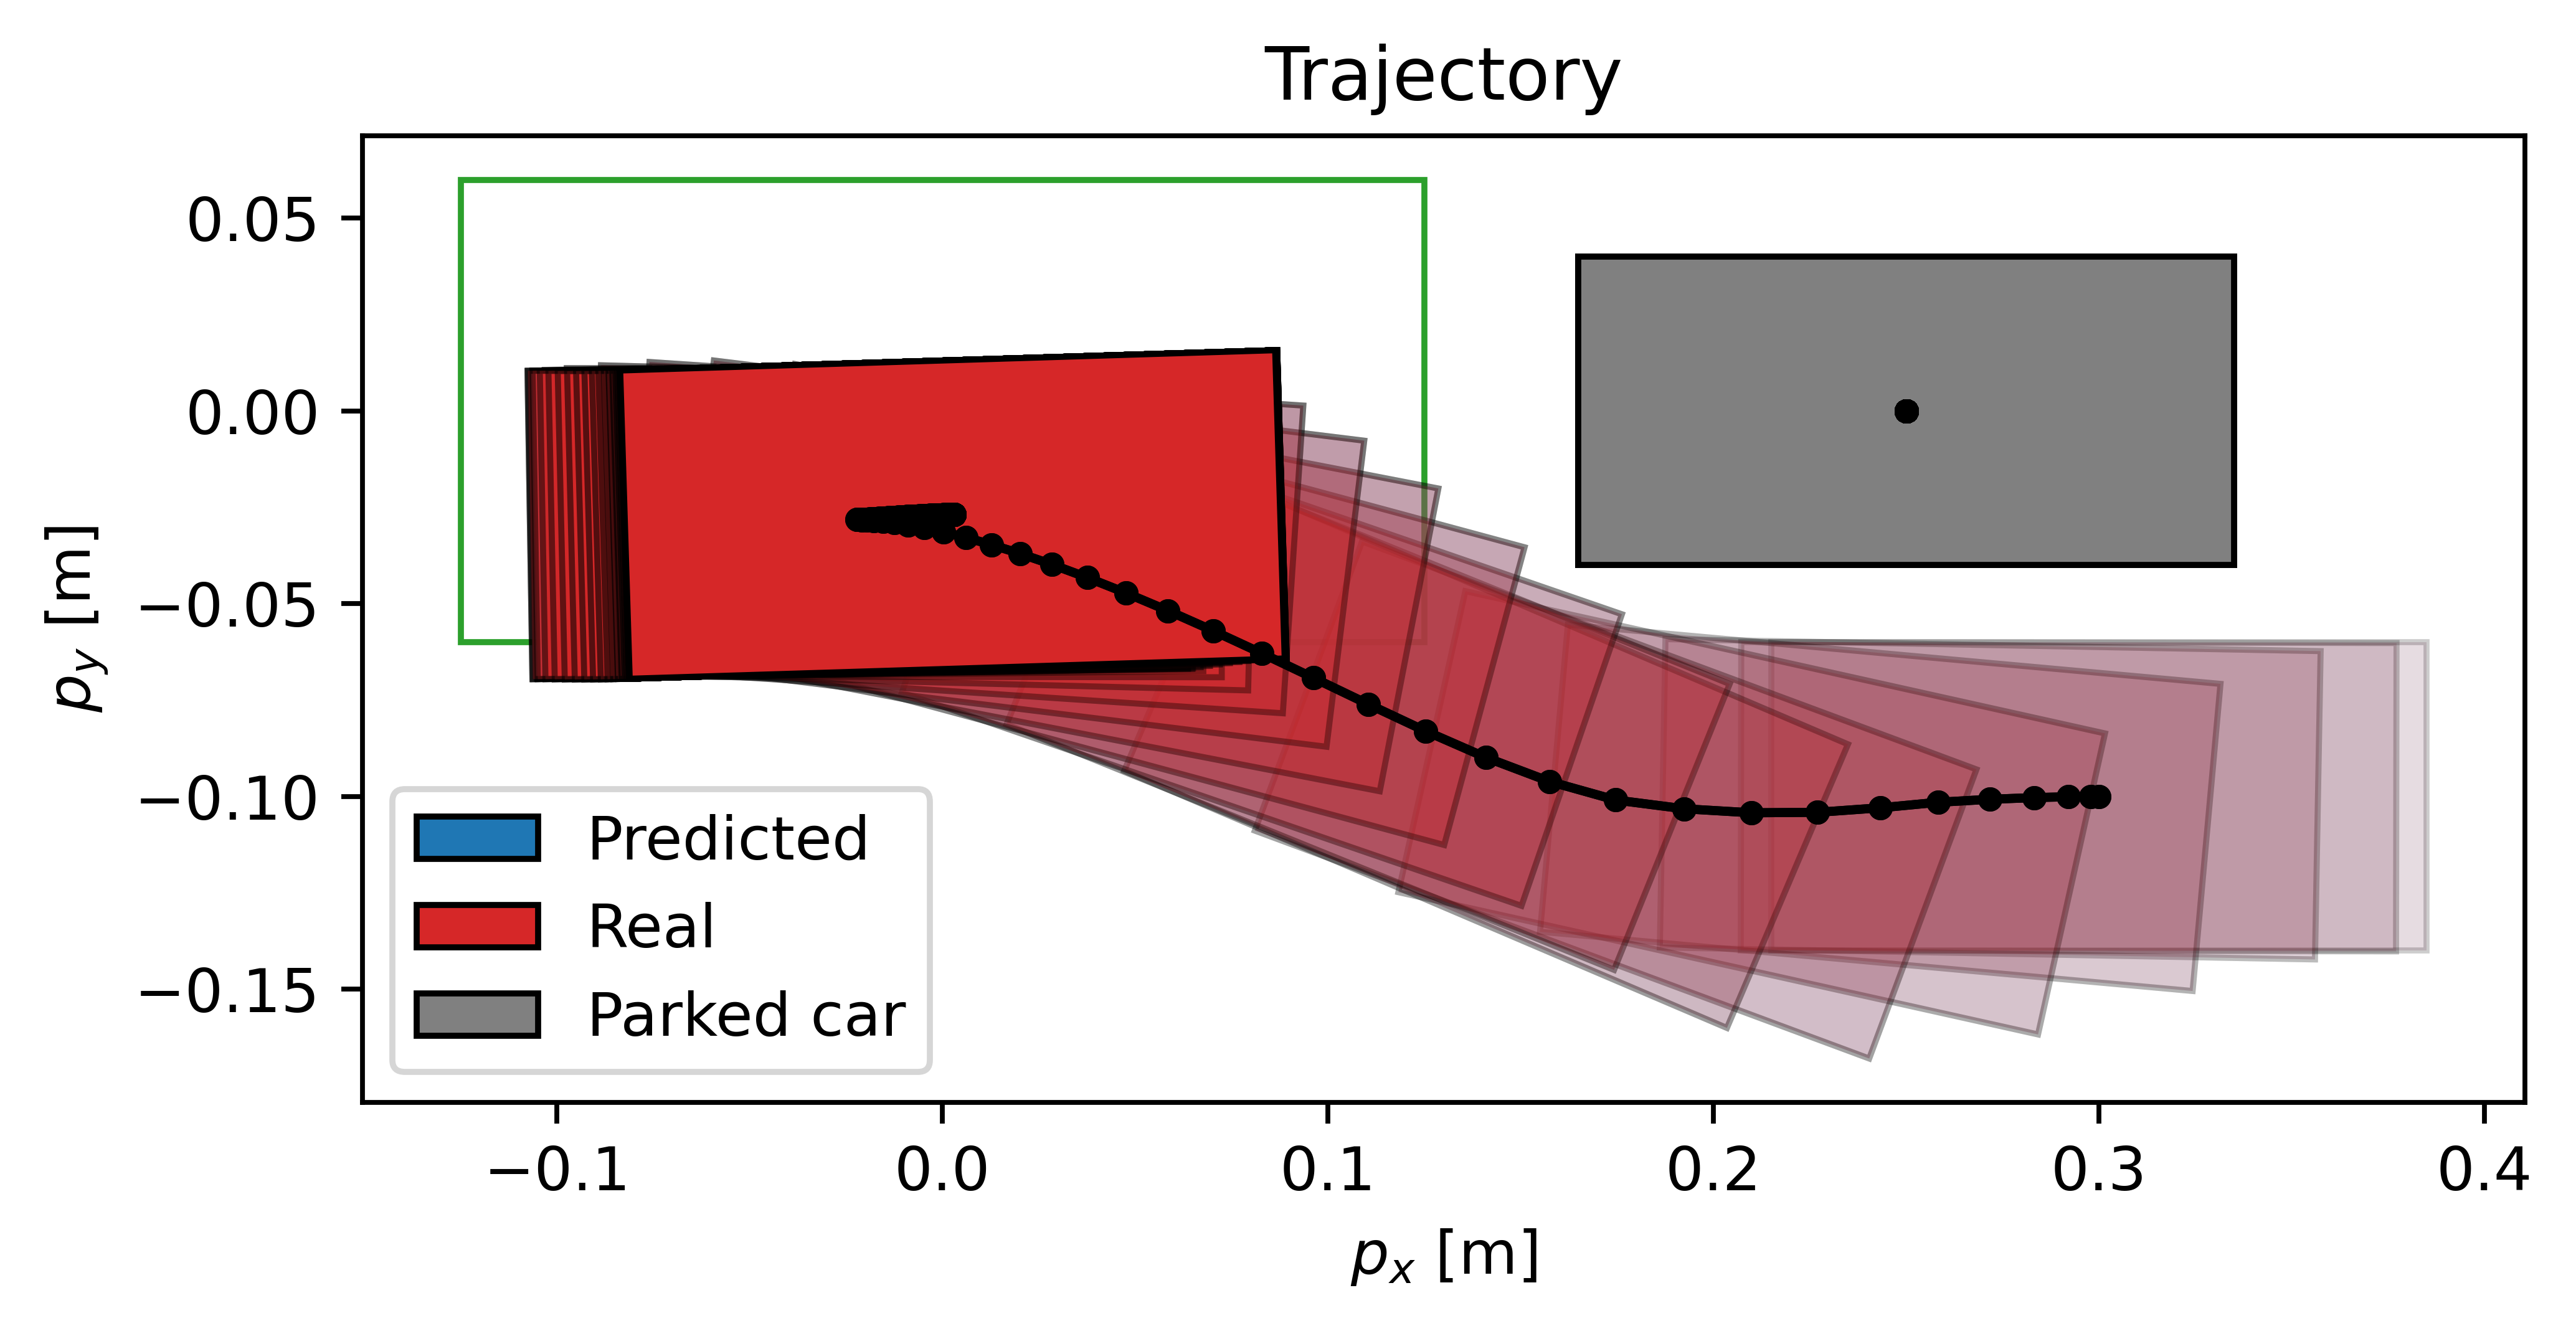
\includegraphics[width=0.7\textwidth]{images/Assignment_44.png}
    \caption{Parking trajectory using default parameters}
    \label{fig:assignment4_4}
\end{figure}



\begin{assignment}
	Play around with the tuning of $Q$, $R$, $N$ or other controller parameters (perhaps even $\nc$, feel free to get creative)
	to obtain a controller which can (without collision) park the vehicle such that it is fully enclosed in the 
	parking spot. Briefly describe your reasoning while tuning, 
	report the final parameters that you changed from the provided defaults
	and illustrate the final result with a plot of the trajectory.
\end{assignment}
\begin{flushleft}
	The tuning parameters were carefully considered in terms of their impact on the car's behavior, followed by a series of experiments conducted to evaluate their practical performance. Here are the results:
\end{flushleft}
\begin{itemize}
    \item $n_c$: affects how closely the car passes by the parked car. Increasing the number of circles improves the approximation of the car by the circles, allowing the car to pass closer to the parked car.
    
    \item $N$: a larger prediction horizon $N$ allows the car to get closer to the desired position (the center of the parking spot $(0,0)$). However, this also increases the computational cost and time.

    \item $Q$: modifying the first two elements on the diagonal of $Q$ helps by increasing the cost associated with the position in $x$ and $y$. Consequently, the car will tend to improve along those directions. Additionally, changing the third element (related to the $yaw$) can also be beneficial.
    
	\item $Q_N$: modifying its elements leads to a greater penalization of the final position of the car additionally pushing the car to reach the origin.
\end{itemize}
Given the observations, the following parameters were changed from the provided defaults and the final tuning is shown in the code below. Using these values, the final position reached by the car is:
\[ [x, y, \text{yaw}, \text{vel}] = [-2.68\exp-06, -3.65\exp-04, -1.28\exp-03, -6.91\exp-07] \]
The final parking trajectory is illustrated in figure \ref{fig:assignment4_5}.
\begin{lstlisting}[style=python]
Q = cs.diagcat(5, 30, 0.05, 0.01)
R = cs.diagcat(0.5, 0.007)
Q_add = cs.diagcat(0, 15, 10, 0)
Q_N = 5 * Q + Q_add
\end{lstlisting}
\begin{figure}[H]
    \centering
    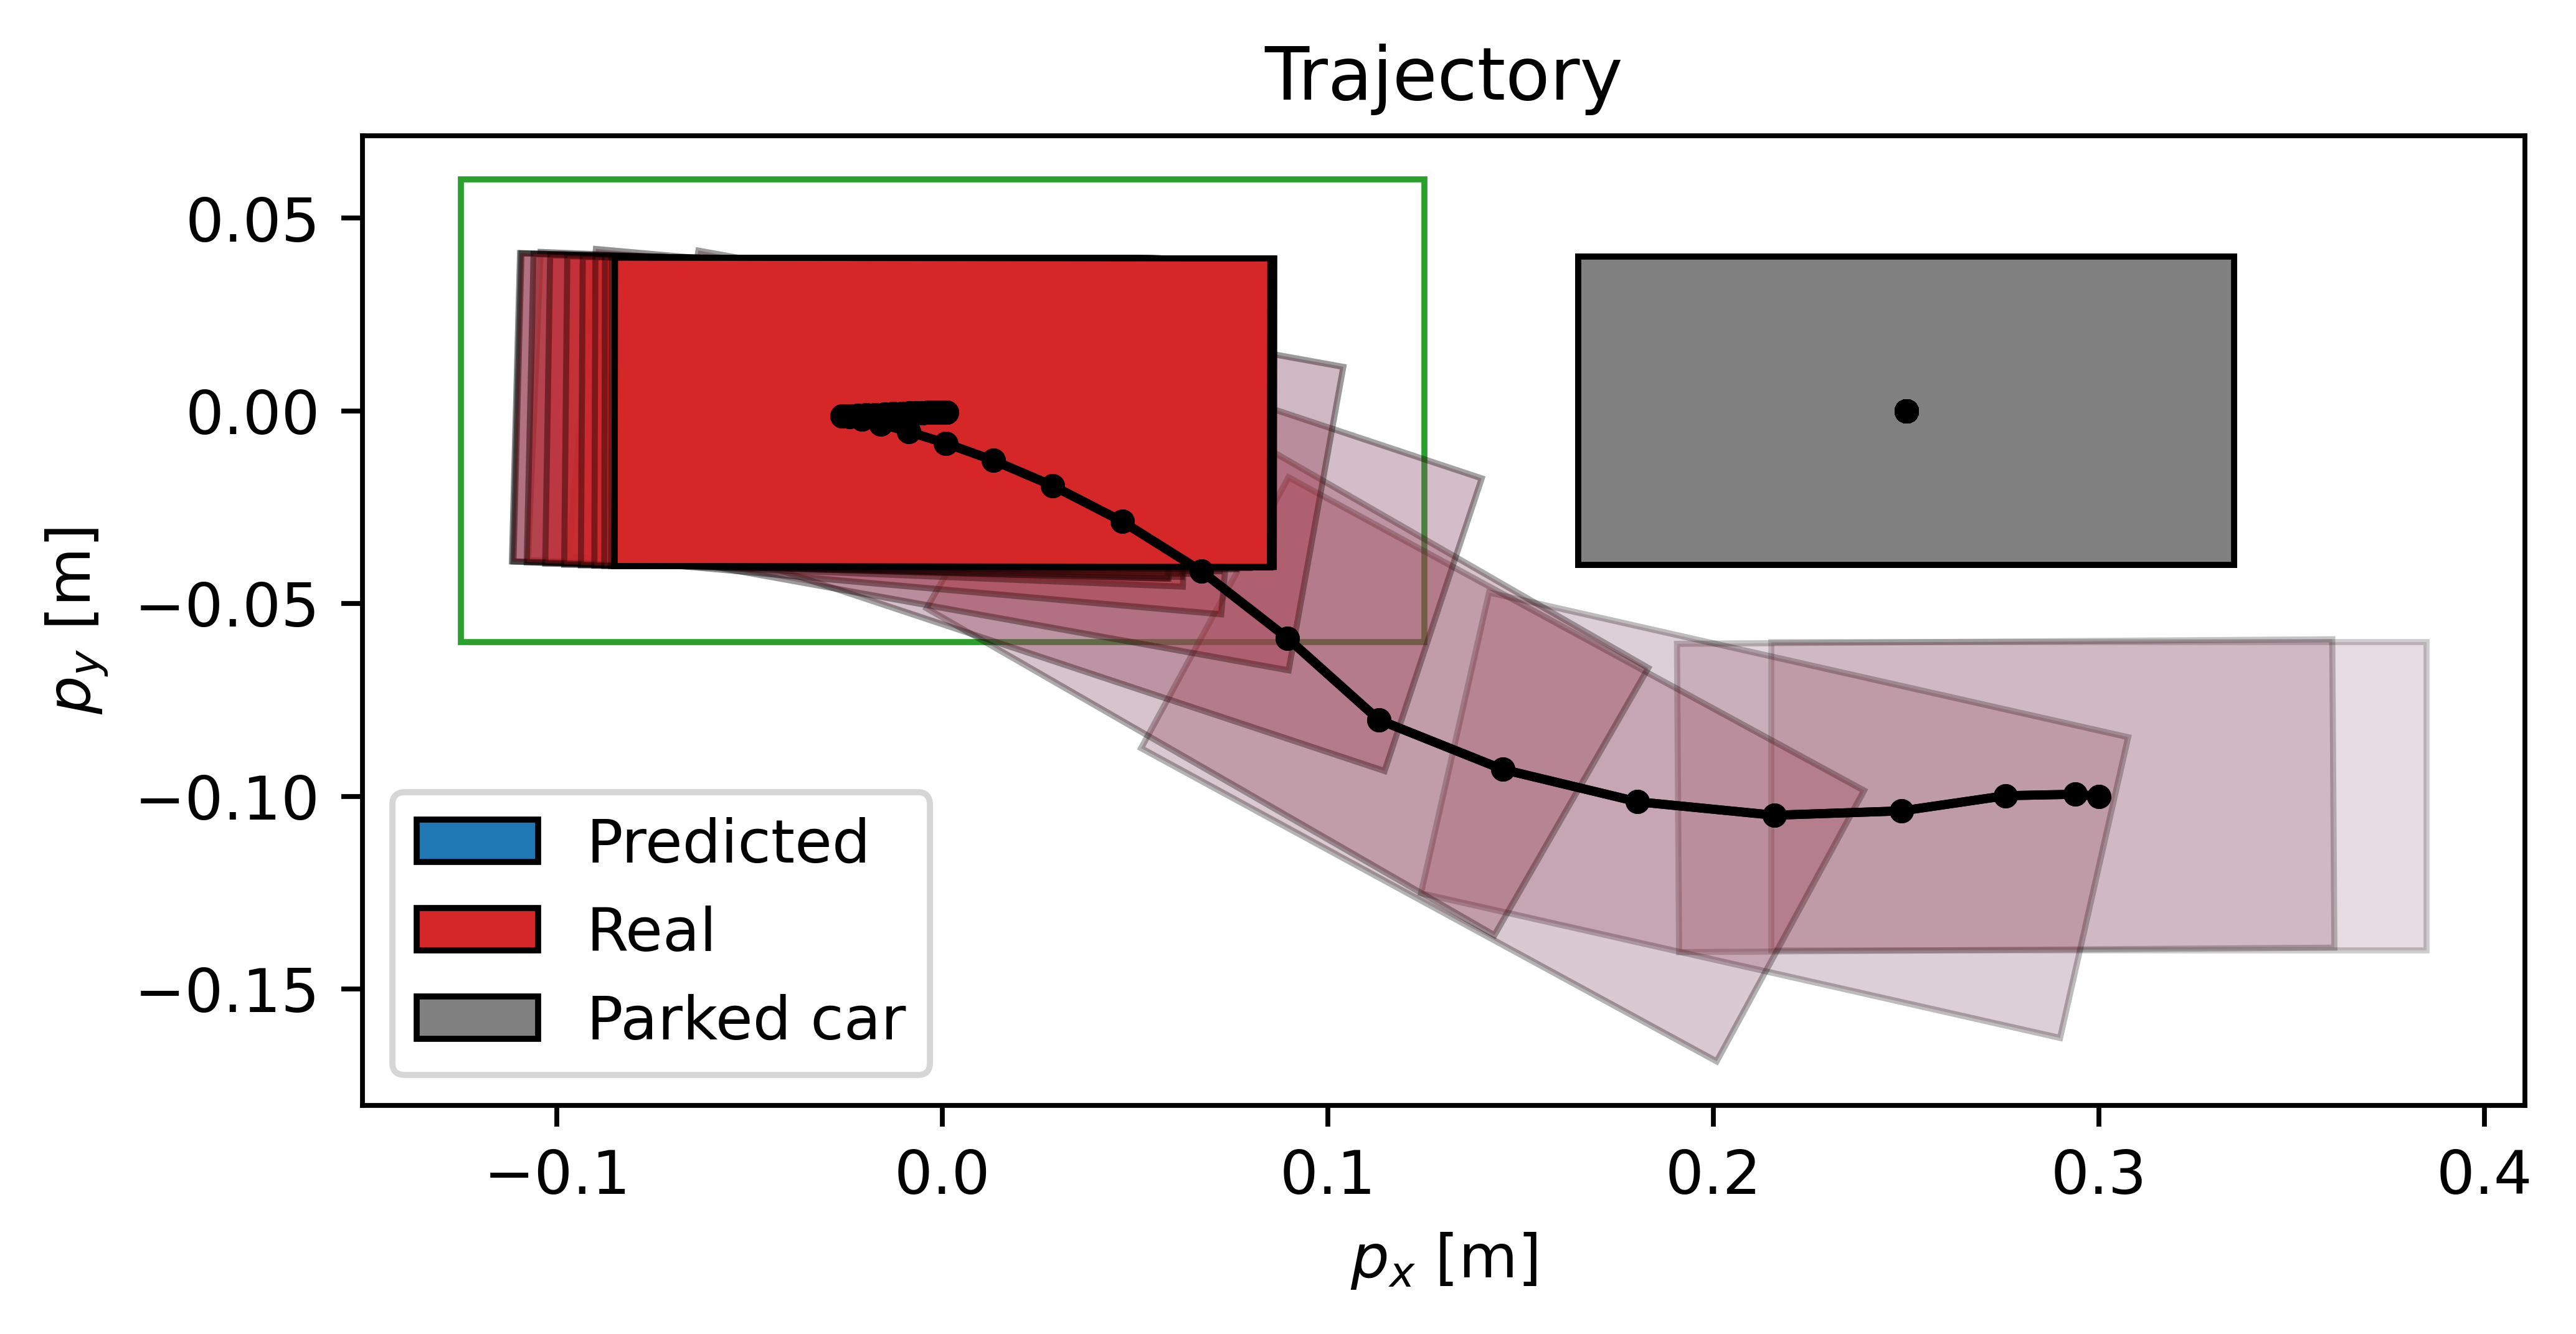
\includegraphics[width=0.7\textwidth]{images/Assignment_45.png}
    \caption{Parking trajectory using custom parameters}
    \label{fig:assignment4_5}
\end{figure}



\begin{assignment}
	Measure your solver time. A quick and easy way to do this is to invoke \texttt{perf\_counter} 
	from the \texttt{time} module before and after your solver call, within the \texttt{\_\_call\_\_} 
	method of your controller. In general, if a solver returns its own time, its usually better to use this instead of measuring the time yourself, in order 
	not to account for overhead in the modeling language. For this assignment, however, you can just use your own timing.
	You can log the solver time by 
	creating a log class 
	\begin{lstlisting}[style=python]
from dataclasses import dataclass
from rcracers.simulator.core import BaseControllerLog, list_field
@dataclass
class ControllerLog(BaseControllerLog): 
    solver_time: list = list_field()
	\end{lstlisting}
	and passing it as \texttt{log} to the \texttt{simulate} method:
	\begin{lstlisting}[style=python]
from rcracers.simulator import simulate
log = ControllerLog()   # Initialize an empty log 
x = simulate(..., log=log) # Simulate 
print(log.solver_time)  # Now the solver times have been written 
	\end{lstlisting}
	Within your solver call, you can then log it like this:
	\begin{lstlisting}[style=python]
from time import perf_counter
def __call__(self, y, log) -> np.ndarray:
	start = perf_counter()
	solution = self.solve(y)
	stop = perf_counter()
	u = self.reshape_input(solution)
	log("solver_time", stop-start)
	return u[0]
	\end{lstlisting}
	Visualize the resulting solver time. Is your MPC controller real-time capable? How did you verify this? If it isn't, finetune your controller to 
	obtain one that is real-time capable and still successfully parks into the parking area.
	Report your final tuning (any value that you changed from the provided defaults)
	and show the timings and state trajectory of the final controller.
\end{assignment}
\begin{flushleft}
	I assumed real-time execution to be any solver time below 75\% of the sampling time $t_s$ (i.e. $0.75 t_s$), this has been implemented in code as can be seen below. 
	To achieve this, I adjusted, from the previously custom parameters, the horizon length $N$ to 8, which reduced the solver time to 0.5 seconds, comfortably meeting the real-time requirement ( $0.5 < 0.6 = 0.75 t_s$ ).
	Below, in figure \ref{fig:assignment4_6} the car's trajectory with this tuning applied can be seen.
\end{flushleft}
\begin{lstlisting}[style=python]
if np.max(log.solver_time) > 0.75 * ts:
	print(f"Solver time: {np.max(log.solver_time):.2f} s")
	print("Not real time execution")
else:
	print(f"Solver time: {np.max(log.solver_time):.2f} s")
	print("Real time execution")
\end{lstlisting}
\begin{figure}[H]
    \centering
    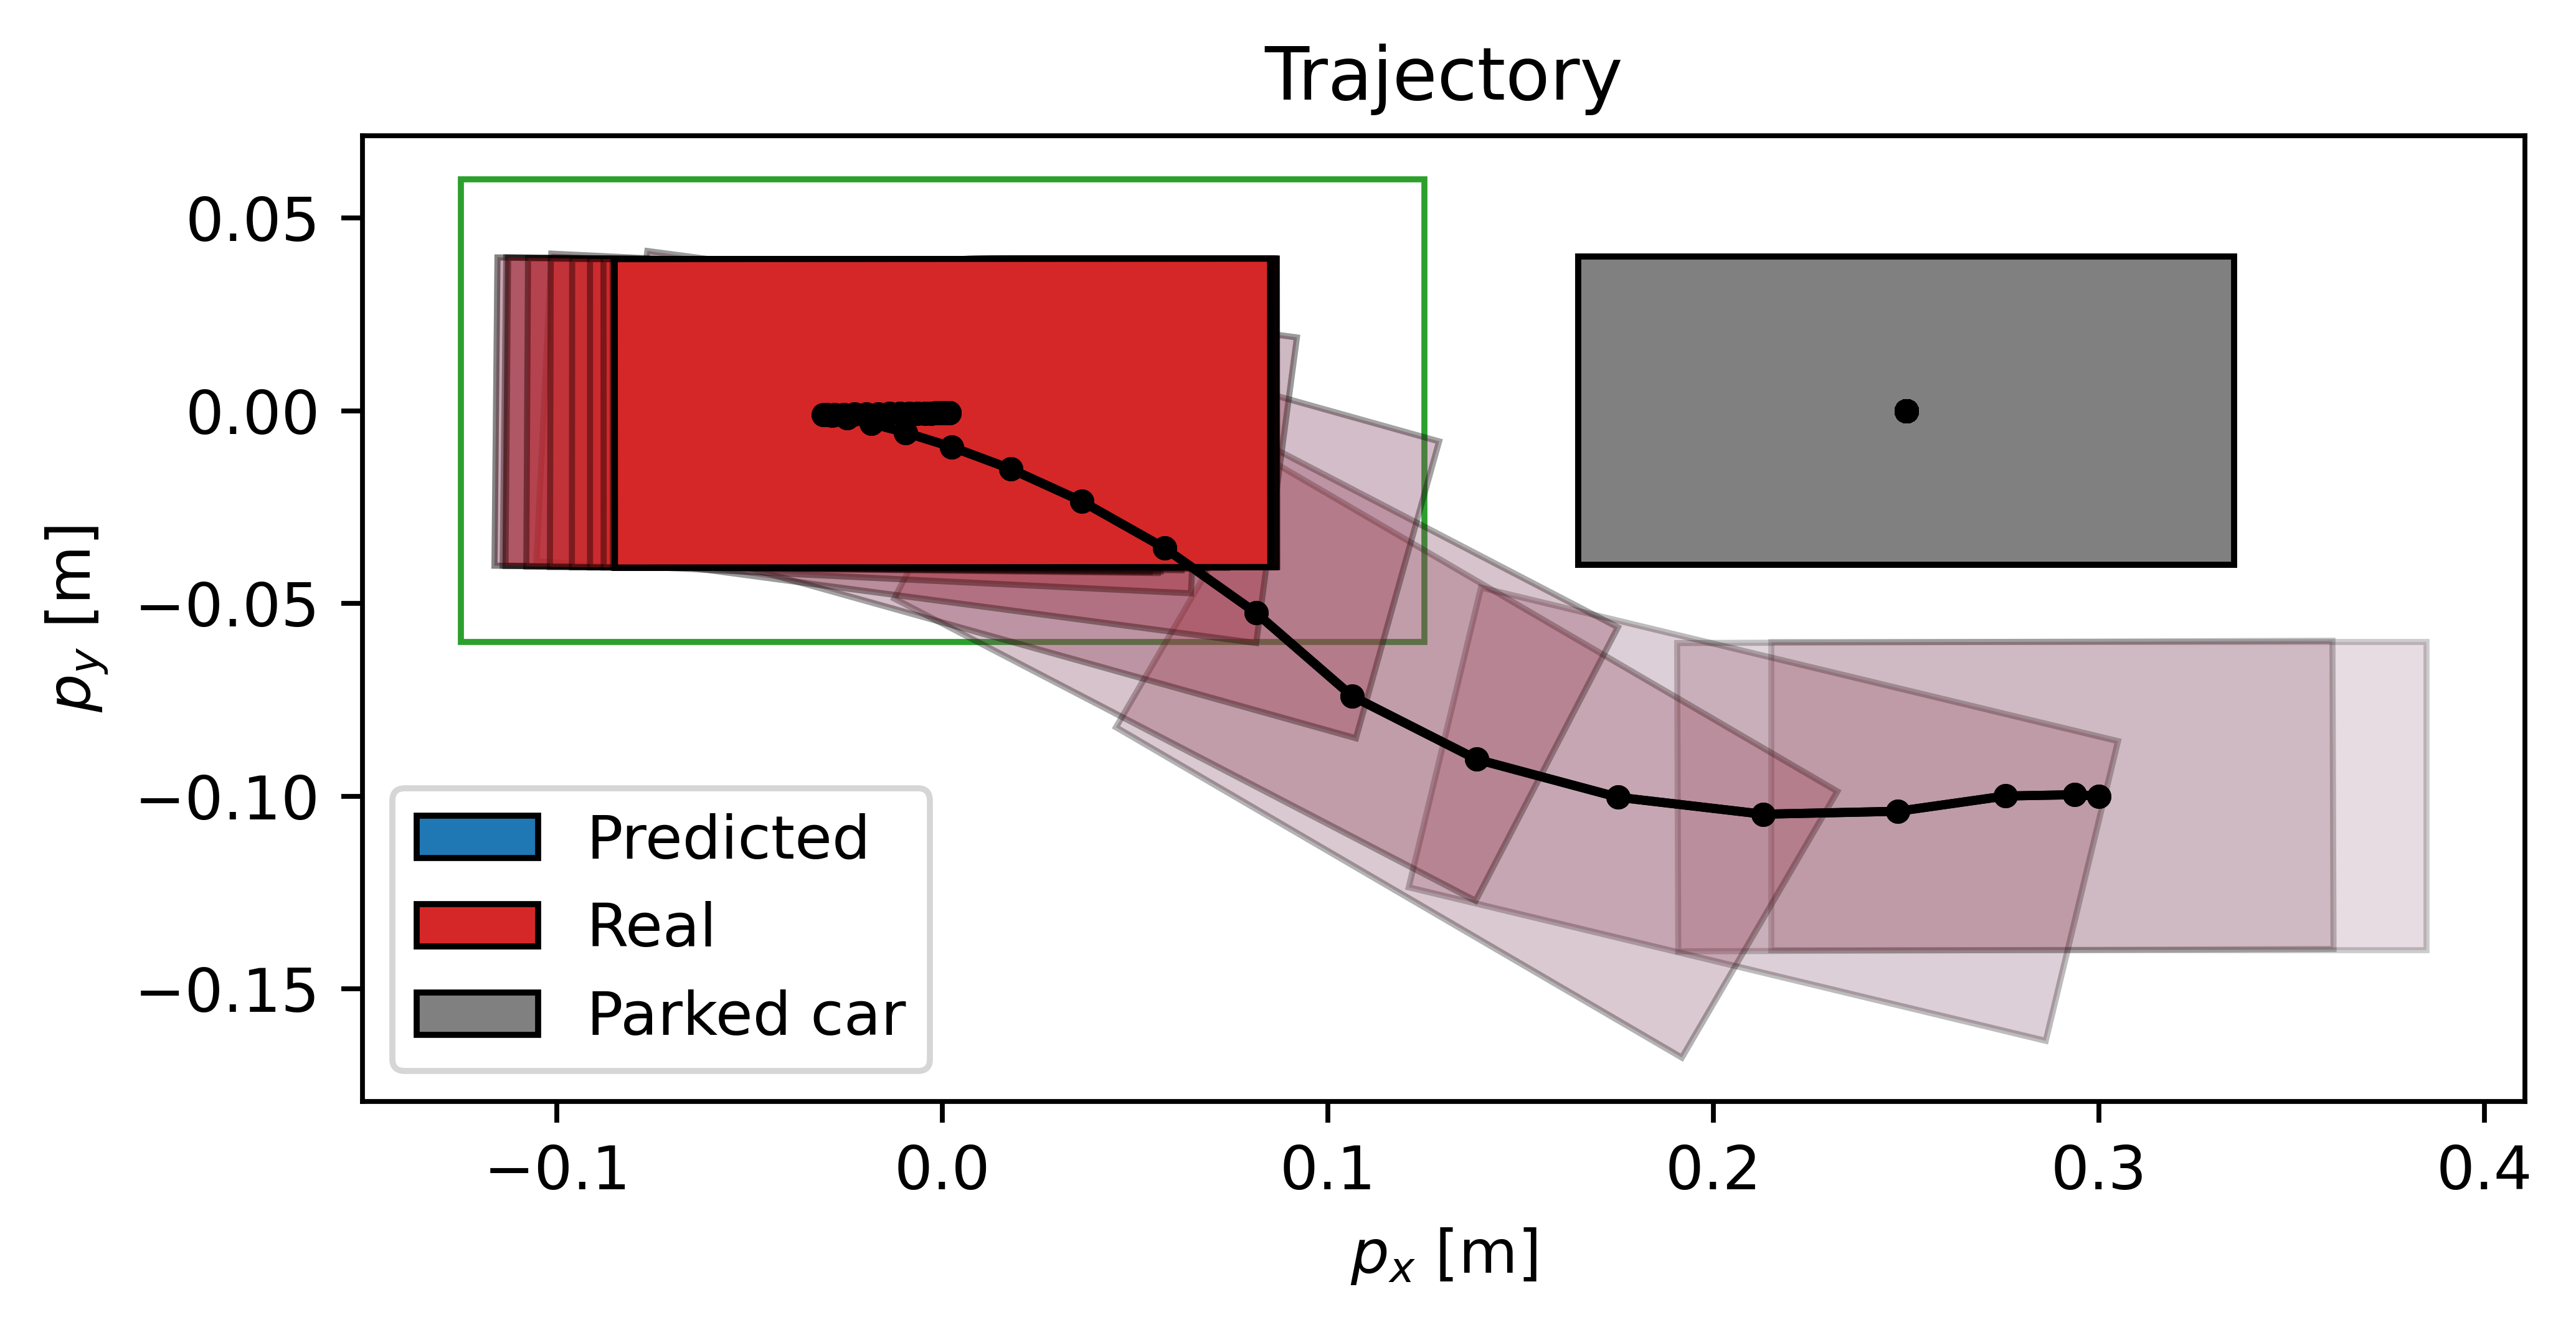
\includegraphics[width=0.7\textwidth]{images/Assignment_46.png}
    \caption{Parking trajectory using custom parameters and real-time execution}
    \label{fig:assignment4_6}
\end{figure}



\newpage
\section{State estimation}
The goal of this assignment is to further improve the MHE you developed in the 
associated exercise session. Specifically right now we only use the data 
provided within the horizon of the MHE optimization problem. Instead 
we would like to use past information as well, which we can do using priors. 
\begin{assignment}
 	We will implement a prior update. Since you already 
    have the EKF iterates available, these can be used to add the \emph{filtering prior update}
    as described in the slides:
    \begin{equation*}
        \Gamma_{T-N}(z) = \frac{1}{2} \nrm{z - \hat{x}_{T-N}}_{(P^-_{T-N})^{-1}}.
    \end{equation*}
    \begin{enumerate}
        \item Note that the \texttt{prior} can already be passed to the provided \texttt{build\_mhe} method:
        \begin{lstlisting}[style=python]
fs, hs = get_system_equations(symbolic=True, noise=True)
loss = lambda w, v: w.T @ w + v.T @ v
solver = build_mhe(loss, f, h, 10, lbx=0.0, ubx=10.0, use_prior=True)

# you can solve the optimization problem as follows:
x, w = solver(P=np.eye(3), x0=np.zeros(3), y=np.zeros((10, 1)))
\end{lstlisting}
        
        \item Alter your \texttt{MHE} class to use \texttt{EKF} internally. 
        Keep in mind that you should produce $\hat{x}_{T-N}$ using only measurements 
        available before time step $T-N$ and the same is true for $P^-_{T-N}$. 
        How many past estimates $\hat{x}_{T-N}$ and $P^-_{T-N}$ should you store 
        internally?

        \item Verify, both for longer horizons ($N = 25$) and shorted ($N=10$) ones
        that the filtering prior improves the behavior. Plot the estimated 
		trajectories.
        
        \item Does clipping the state estimates in the \emph{EKF} aid the 
        performance? Plot the result.
    \end{enumerate}
    \solution{See \texttt{MHE} in \texttt{session4\_sol.py}.} 
\end{assignment}
\begin{enumerate}
	\item The prior can be passed to the \texttt{build\_mhe} method as follows:
	\begin{lstlisting}[style=python]
	def build(self, horizon: int):
        return build_mhe(
            self.loss,
            self.f,
            self.h,
            horizon,
            lbx=self.lbx,
            ubx=self.ubx,
            use_prior=True
        )
	\end{lstlisting}
	
	\item The \texttt{MHE} has been modified in the following way to implement internally an \texttt{EKF} that to produce $\hat{x}_{T-N}$, and $P^-_{T-N}$, uses only the measurements available before time $T-N$. 
	The number of past estimates to store was found to be equal to the horizon length, $N$.
	\begin{lstlisting}[style=python]
		def __call__(self, y: np.ndarray, log: LOGGER):
        # Store the new measurement
        self.y.append(y)
        if len(self.y) > self.horizon:
            self.y.pop(0)

        # Update EKF with the new measurement
        for y in self.y:
            self.ekf(y)

        # Store past estimates of x and P
        self.x_past.append(self.ekf.x.copy())
        self.P_past.append(self.ekf.P.copy())
        if len(self.x_past) > self.horizon:
            self.x_past.pop(0)
            self.P_past.pop(0)

        # Use EKF state as initial guess for MHE
        if len(self.y) < self.horizon:
            solver = self.build(len(self.y))
            initial_state = self.x_past[0]
            P = self.P_past[0]
        else:
            solver = self.solver
            initial_state = self.x_past[-self.horizon]
            P = self.P_past[-self.horizon]

        # Update MHE
        x, _ = solver(P, initial_state, self.y)

        # update log
        log("x", x[-1, :])
        log("y", y)
	\end{lstlisting}
	
	\item The obtained plots for $N = [10, 25]$ are shown in figures \ref{fig:assignment51_1} and \ref{fig:assignment51_2}.
	\begin{figure}[H]
		\centering
		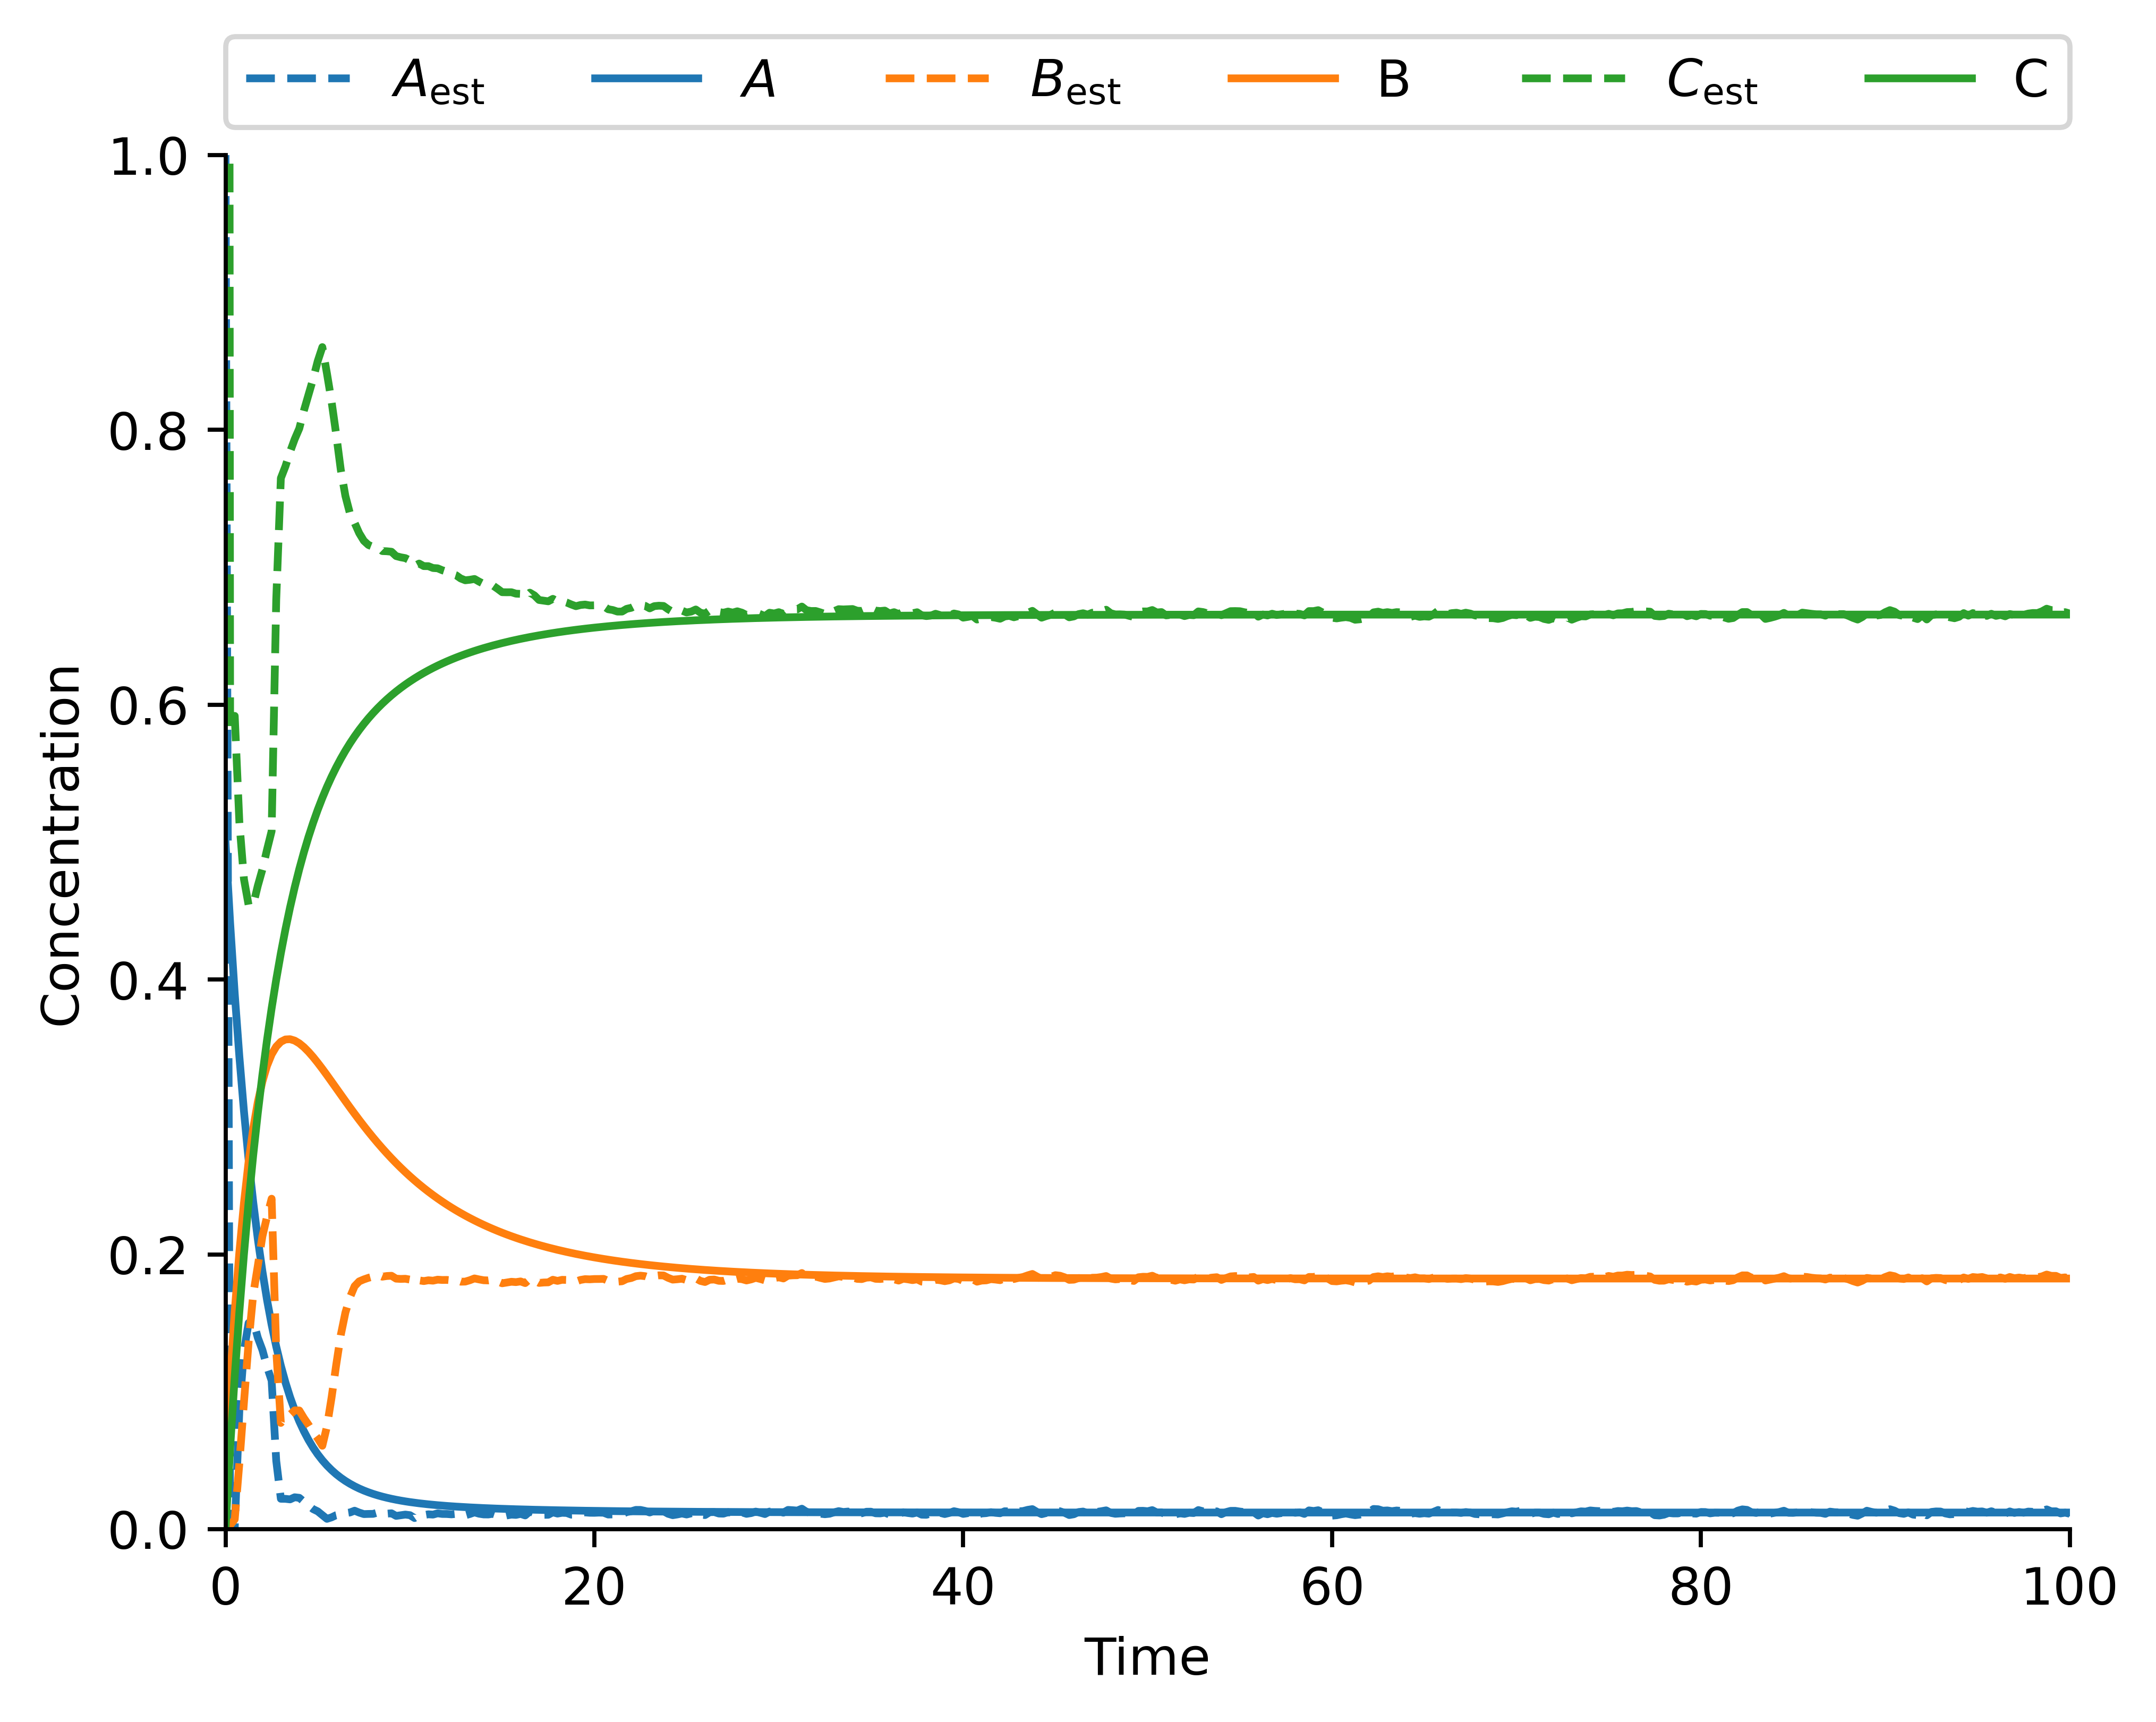
\includegraphics[width=0.7\textwidth]{images/Assignment5_N=10_False.png}
		\caption{States and their estimation evolution - N = 10}
		\label{fig:assignment51_1}
	\end{figure}
	\begin{figure}[H]
		\centering
		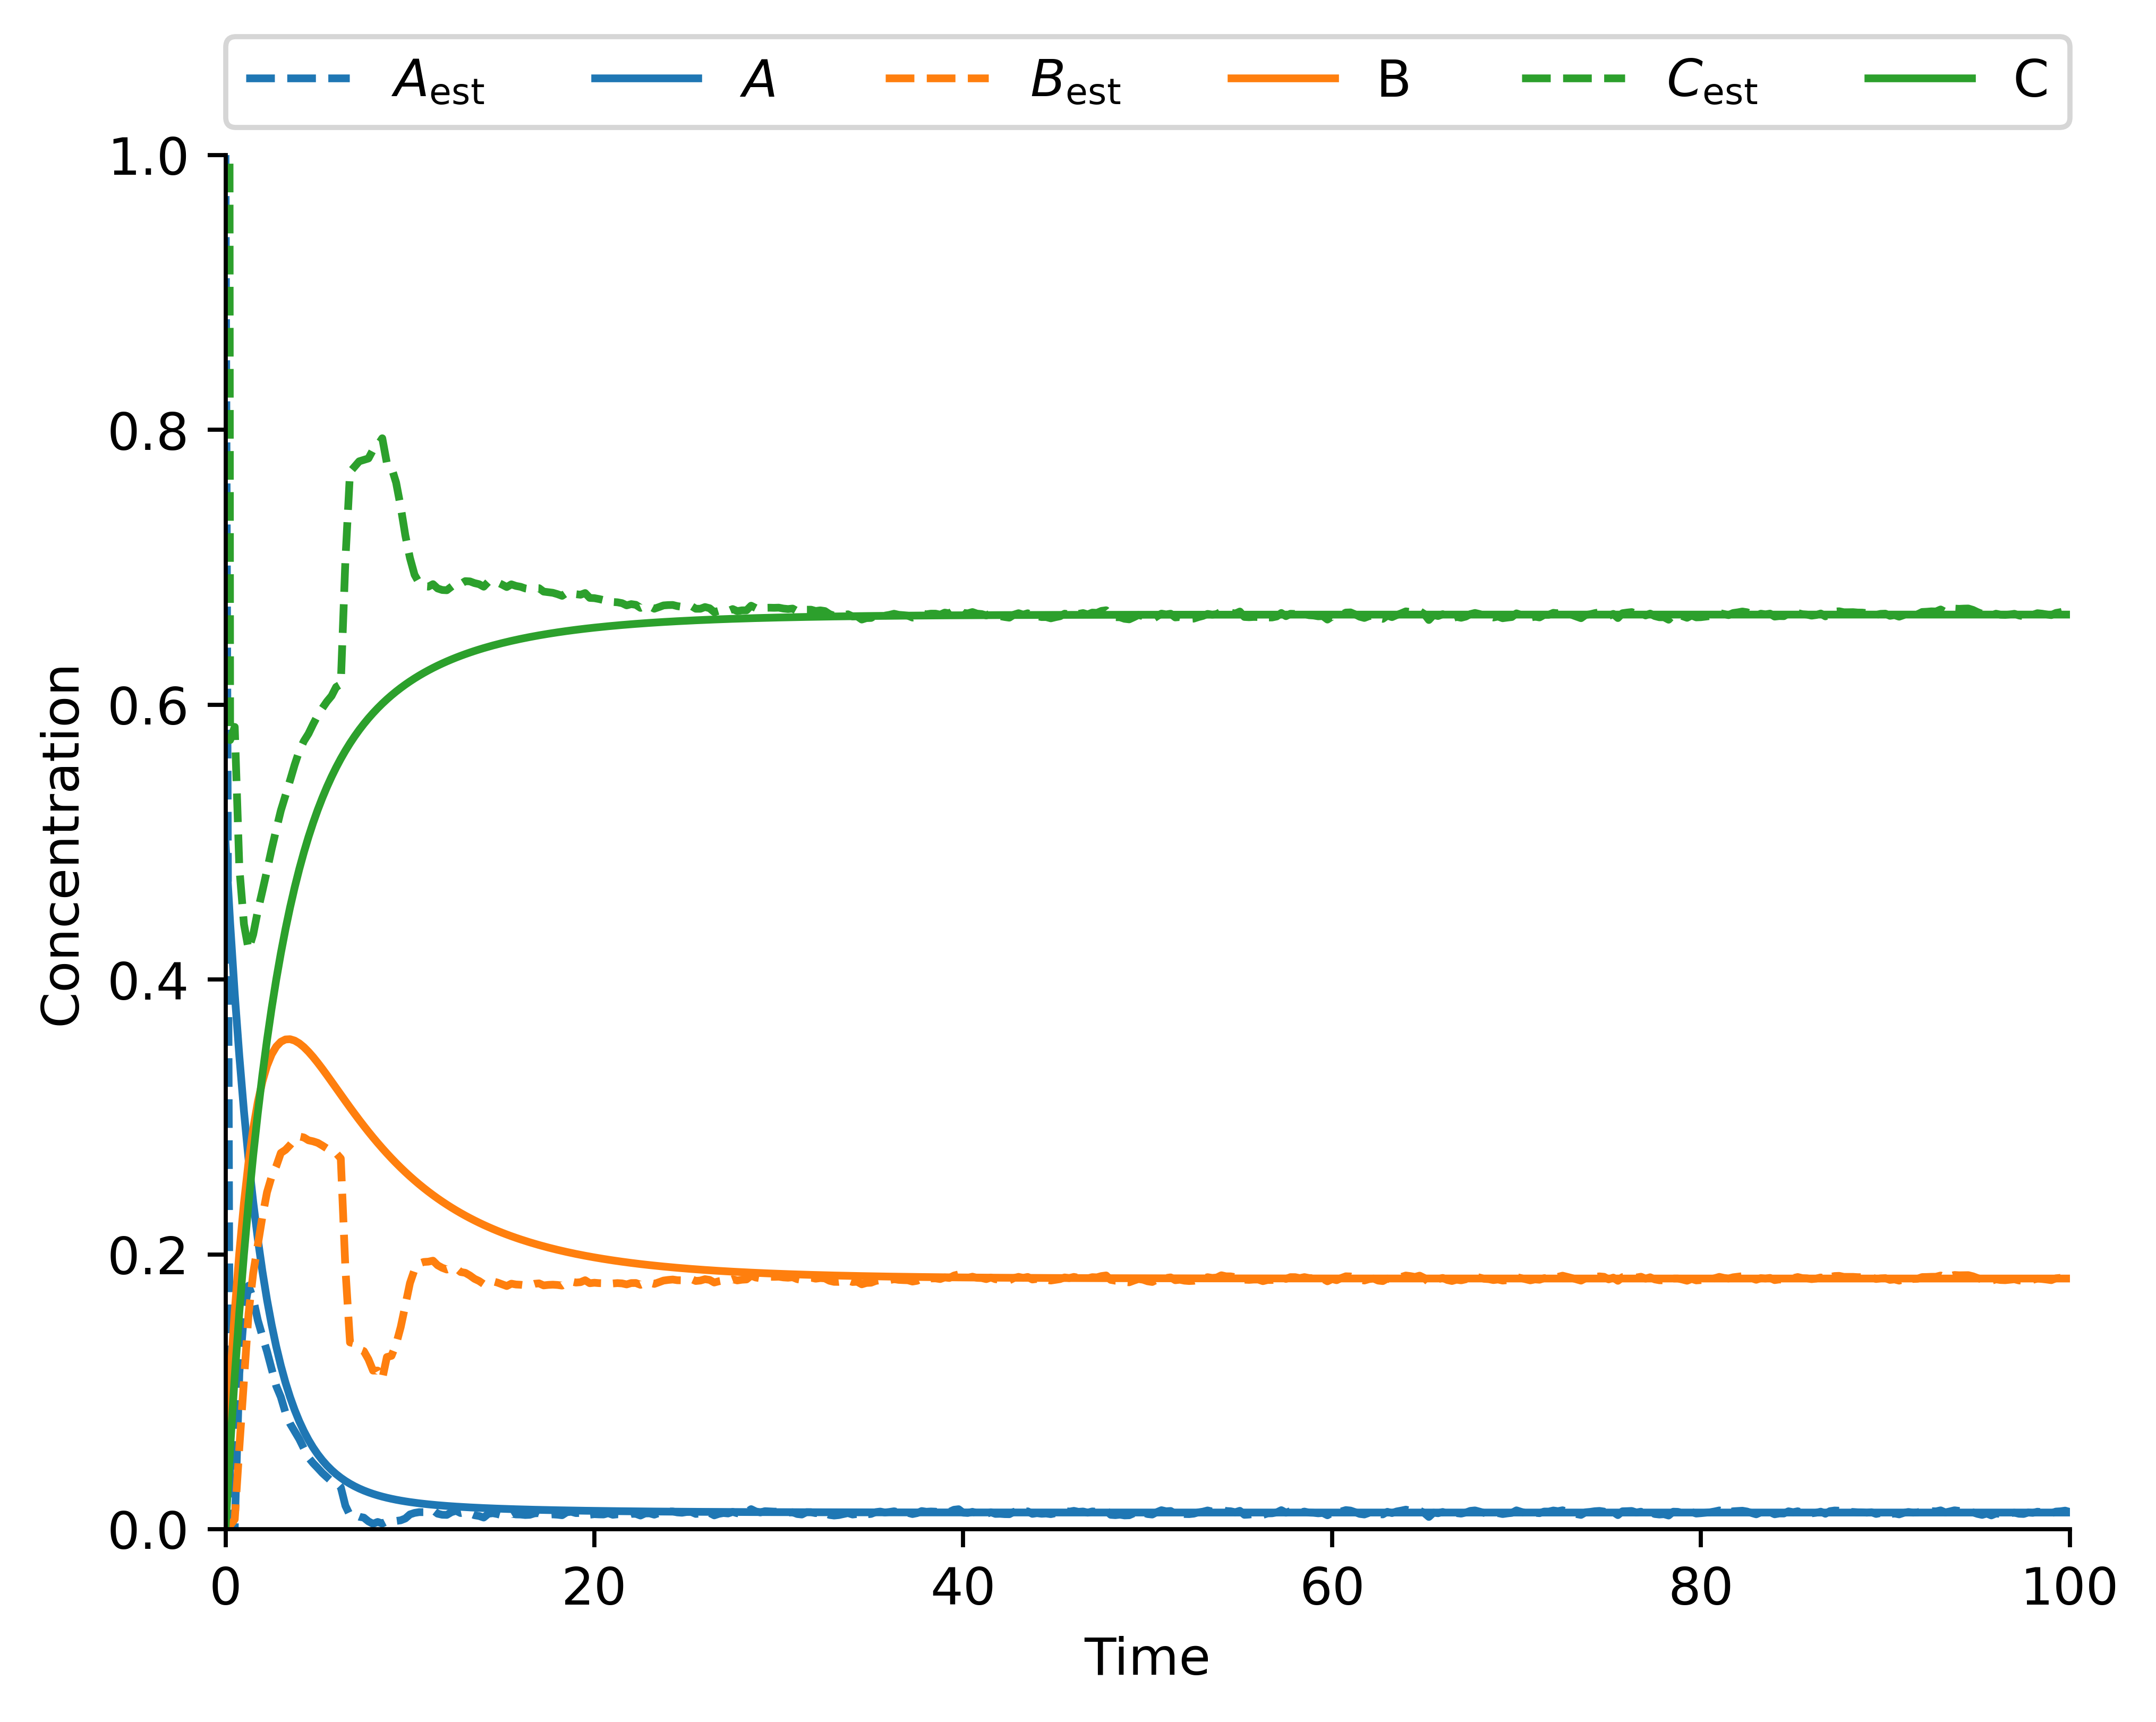
\includegraphics[width=0.7\textwidth]{images/Assignment5_N=25_False.png}
		\caption{States and their estimation evolution - N = 25}
		\label{fig:assignment51_2}
	\end{figure}
	
	\item Clipping the state estimates in the \texttt{EKF} aids the performance making sure that non positive actions are avoided. 
	Figures \ref{fig:assignment52_1} and \ref{fig:assignment52_2} show the state evolution for both the horizon lenghts with clipping.
	\begin{figure}[H]
		\centering
		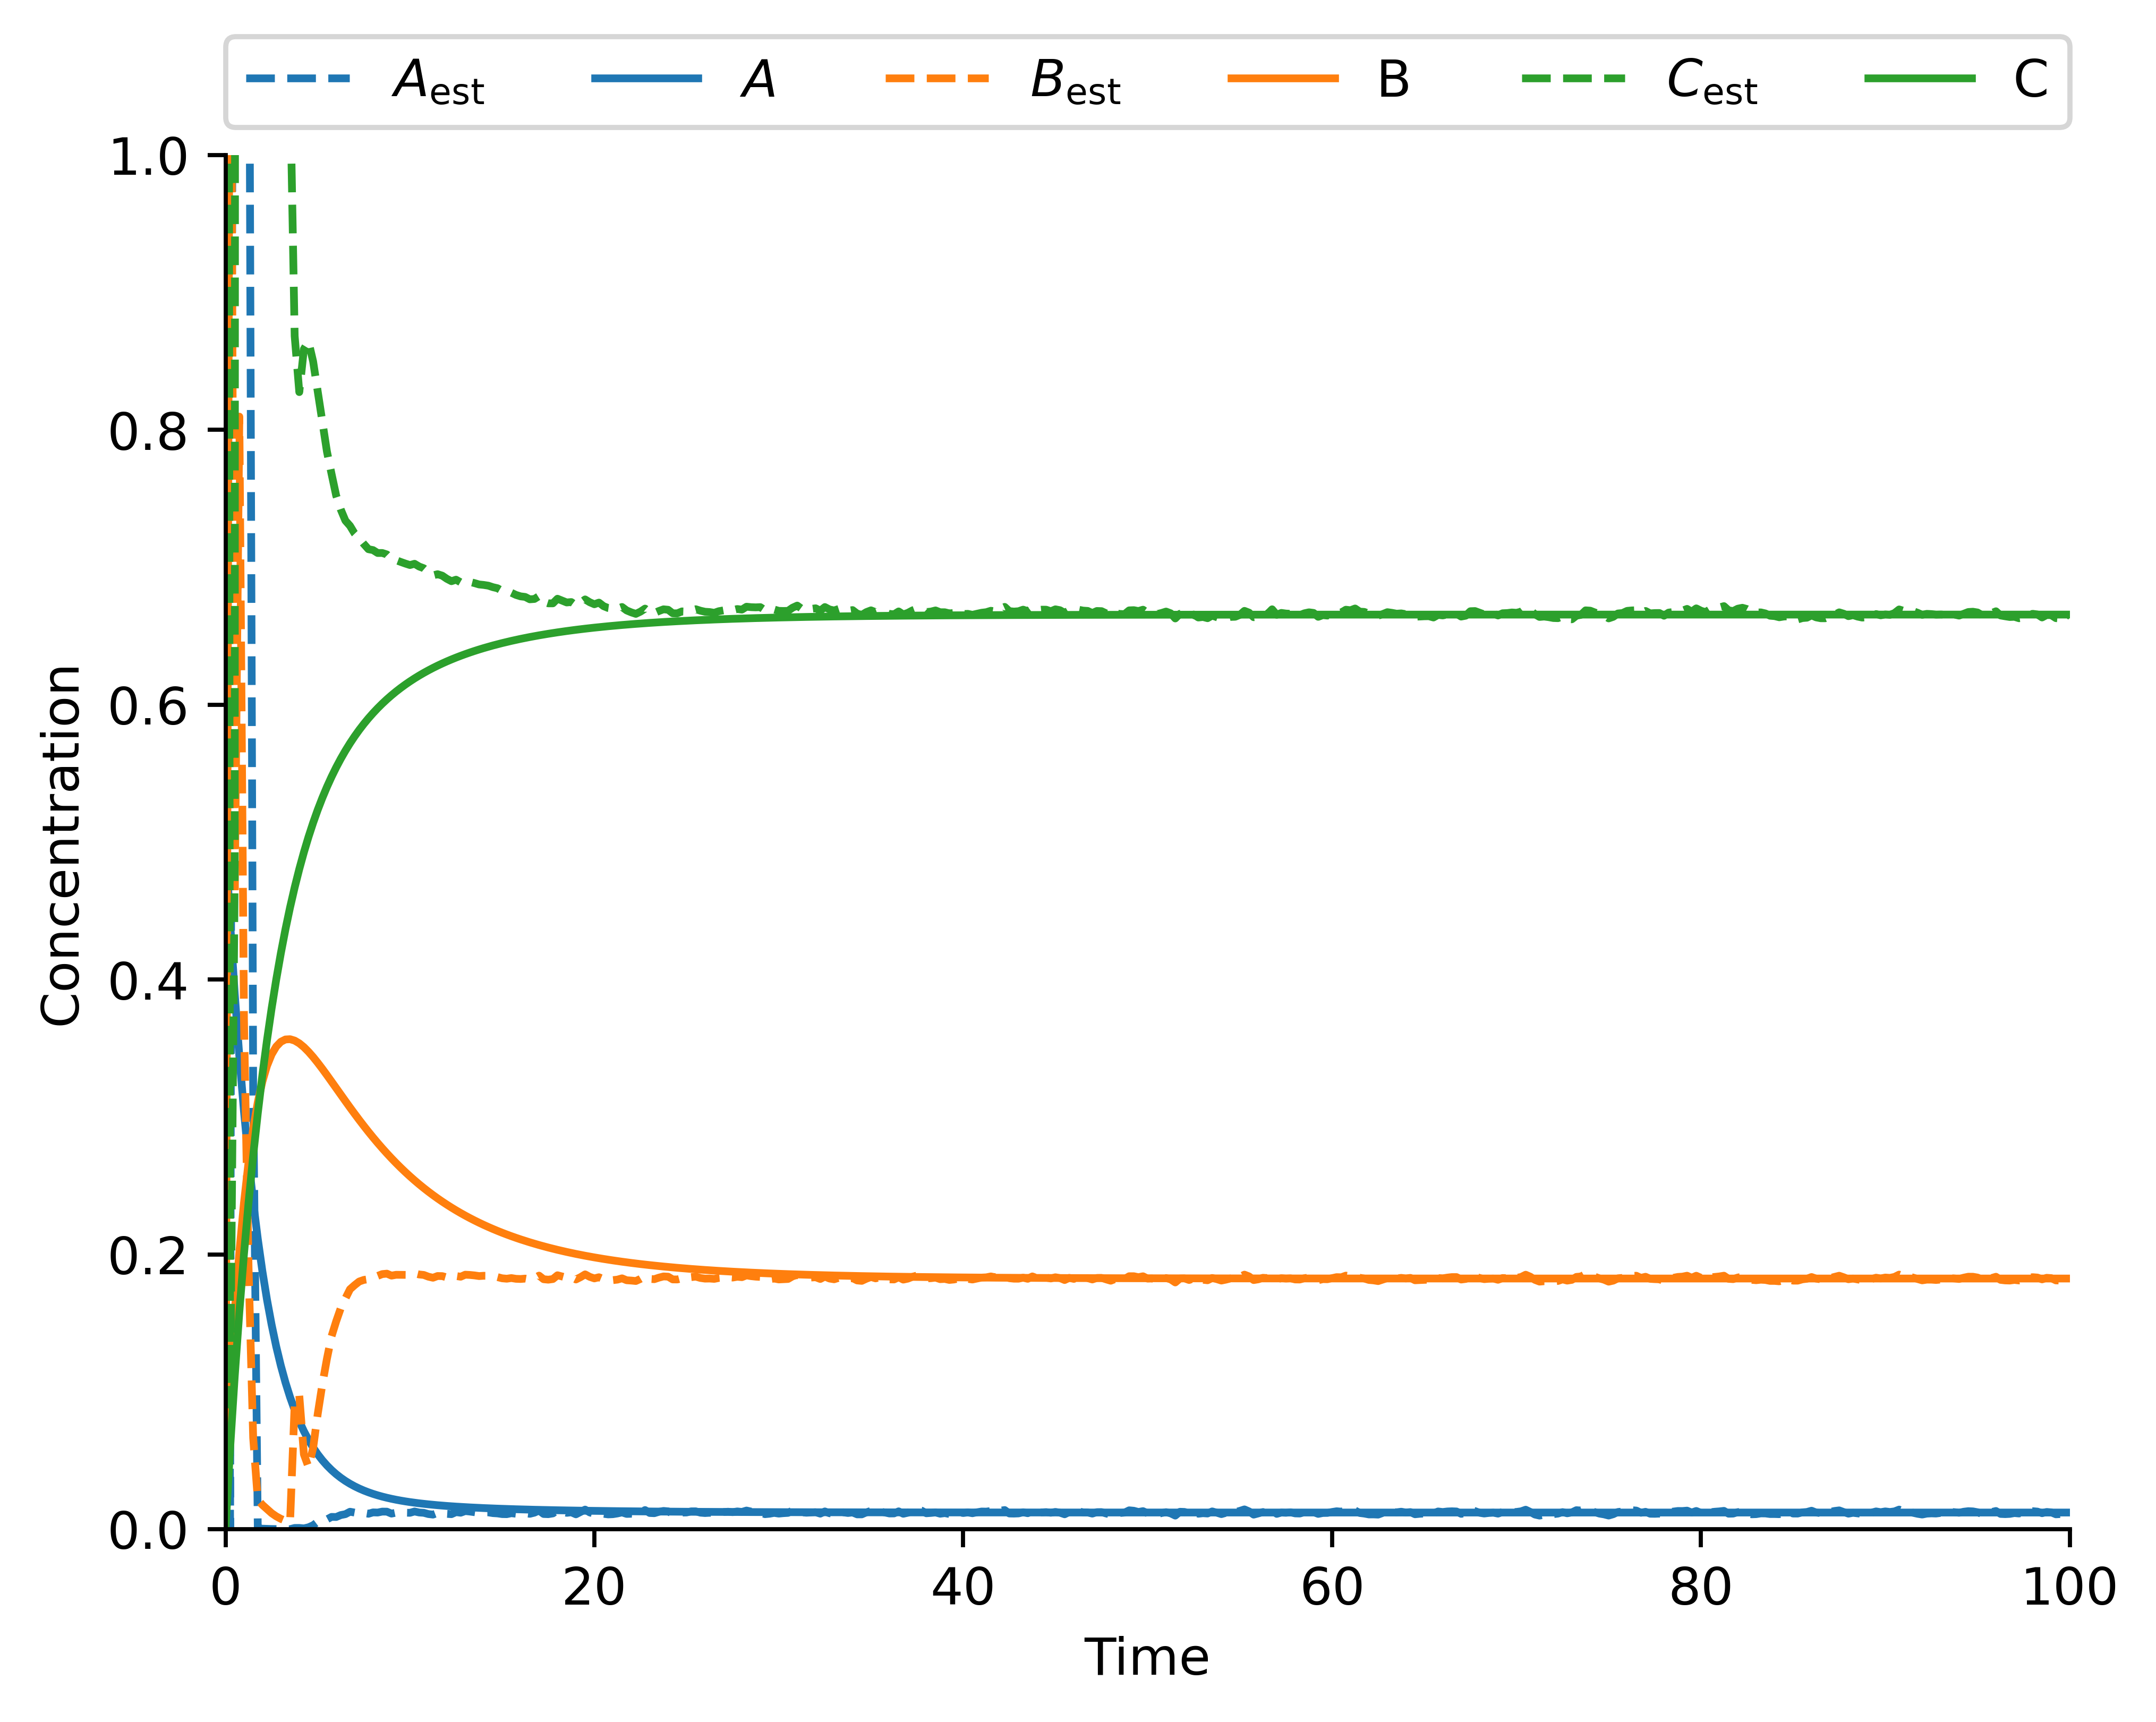
\includegraphics[width=0.7\textwidth]{images/Assignment5_N=10_True.png}
		\caption{States and their estimation evolution - N = 10 + Clipping}
		\label{fig:assignment52_1}
	\end{figure}
	\begin{figure}[H]
		\centering
		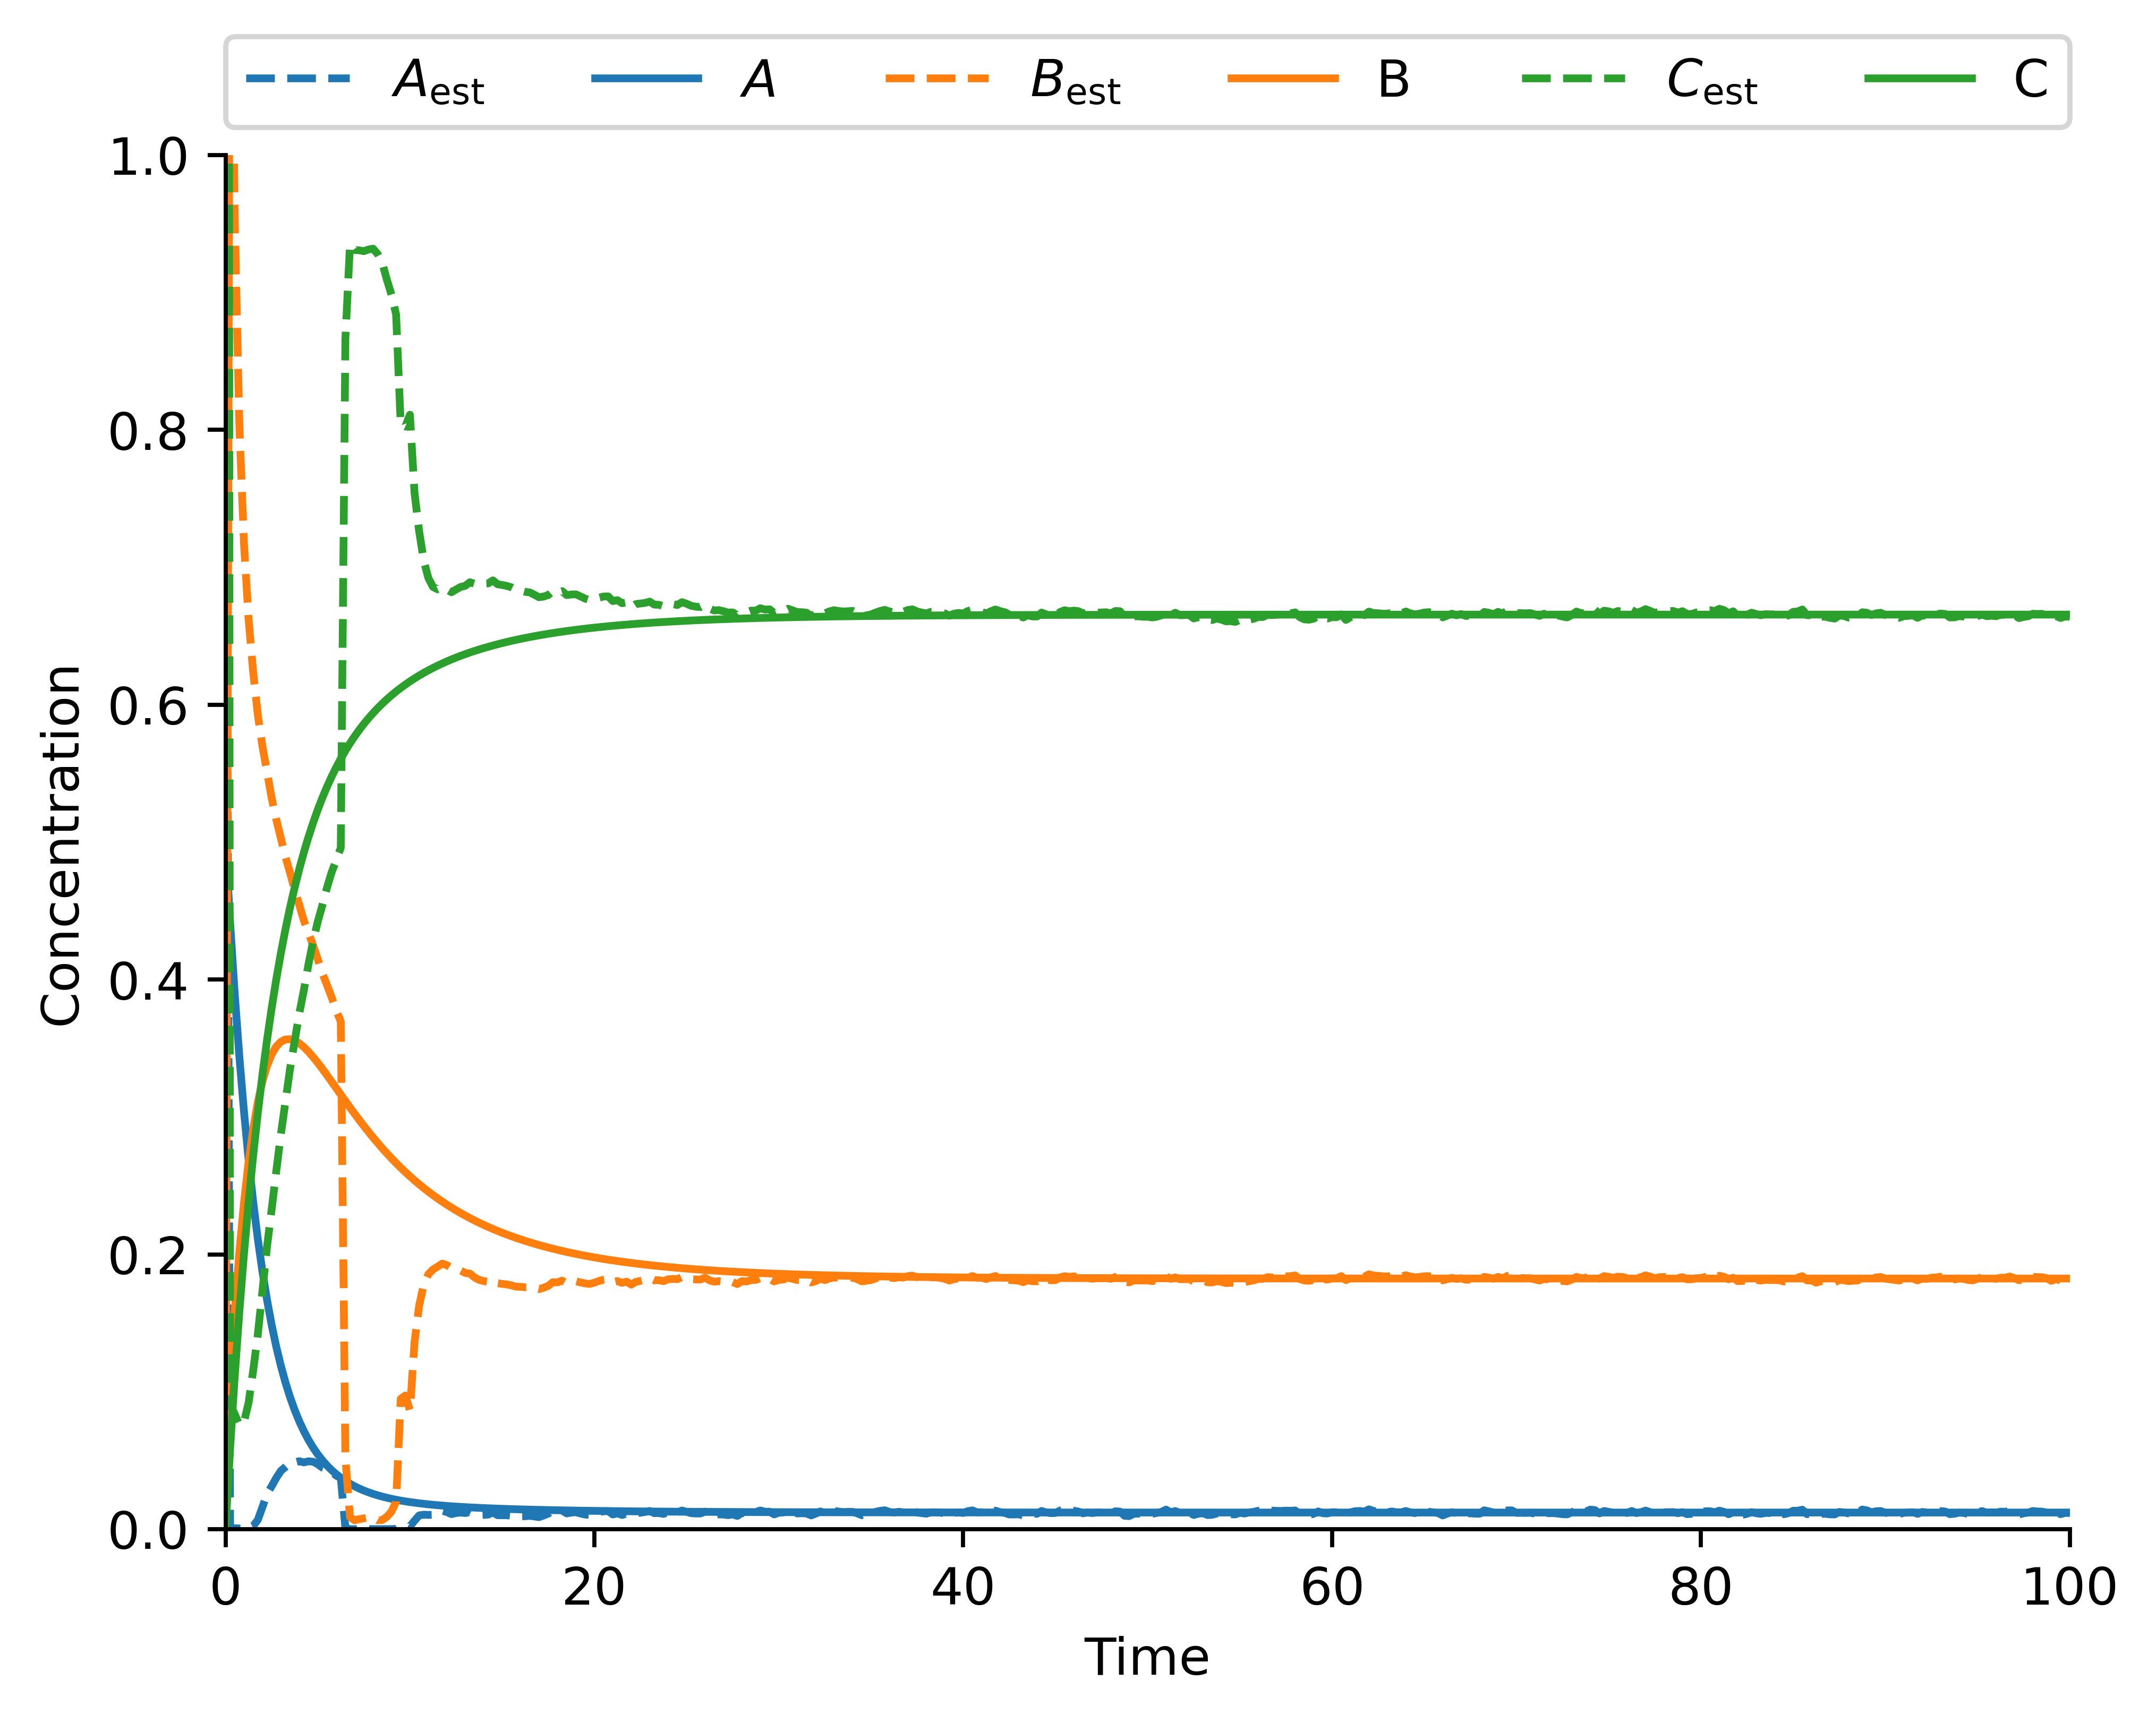
\includegraphics[width=0.7\textwidth]{images/Assignment5_N=25_True.png}
		\caption{States and their estimation evolution - N = 25 + Clipping}
		\label{fig:assignment52_2}
	\end{figure}
\end{enumerate}




\newpage 
\section{Optimization}

The goal of this assignment is to get familiar with methods for solving nonlinear MPC problems. 
Due to the nonlinearity of the dynamics, the OCP
will be nonconvex and therefore, the methods from during the session will no longer be applicable. 

The given code (\texttt{problem.py}), 
defines a few test problems and some data-structures that 
you can use to build your nonlinear solver. Have a brief 
look at this file, and read the comments therein
to get acquainted with the provided ingredients.
You will not be required to make any changes 
in this file.  

A scaffolding for your own implementation is given 
in \texttt{template.py}. Throughout this 
assignment, you will fill in the blanks in this file, 
to finally obtain a solver for nonlinear optimal control problems.

\subsection{Building the solver}
We will build a Newton-Lagrange method 
for multiple shooting (i.e., simultaneous approach).

\begin{assignment}
	Implement the Newton-Lagrange method (SQP) by 
	completing the auxiliary functions used by \texttt{newton\_lagrange} in 
	the provided template. Particularly, 
	the functions \texttt{lqr\_factor\_step}, \texttt{lqr\_solve\_step}
	and \texttt{update\_iterate} need to be implemented. The former two functions should implement 
	Algorithms 2 and 3 in the related lecture slides. 
	In \texttt{update\_iterate}, you can for now assume that the option \texttt{linesearch} is \texttt{False}.

	Run the function \texttt{test\_linear\_system} and present the output.
	This function calls your SQP solver on a problem involving 
	a linear system. Is the output what you expect? Why?
\end{assignment}
\begin{flushleft}
	Expected convergence in 1 iteration as the system is linear, but reached in 2 iterations. 
\end{flushleft}
\begin{lstlisting}[style=python]
	it.    0 | JN = 1.51e+04 | ||h||2 = 1.25e-13
	it.    1 | JN = 1.51e+04 | ||h||2 = 1.07e-13
	Converged
\end{lstlisting}



\subsection{Nonlinear test case}
Now that you have tested your implementation on a linear system,
we will move on to a nonlinear example.

Consider the continuous time dynamics 
\[
\begin{aligned}
  \dot{x}_1 &=  10(x_2 - x_1) \\
  \dot{x}_2 &= x_1(u - x_3) - x_2 \\
  \dot{x}_3 &= x_1x_2 - 3x_3 
\end{aligned}
.\] 
which are discretized using the foward Euler scheme. 
This system is already implemented in \texttt{problem.py} under \texttt{ToyDynamics}. 
The problem that you can pass to your SQP solver is described by \texttt{ToyProblem}.

\begin{assignment} \label{assgn:62}
	Construct an initial guess of all zeros for the inputs, the states and the costates.
	However, for the states, keep in mind that the first entry must be the provided initial 
	state, i.e., \texttt{problem.x0}. Run your solver with this 
	initial state. Give the cost and constraint violation of the last iterate
	(printed automatically using the \texttt{Logger} class in \texttt{given.problem}). 
	Use the provided \texttt{animate\_iterates} function to animate the states and inputs over the iterates and to export a 
	figure of the final solution. Add this plot in your report. Does your solution look plausible?
\end{assignment}
\begin{flushleft}
	The obtained plot of the evolution of the states figure \ref{fig:assignment6_2} of the nonlinear system, appears plausible. 
	The state trajectories are consistent with the expectations for a nonlinear system subject to SQP optimization. They evolve in a smooth and predictable manner, avoiding abrupt or erratic transitions.
	Moreover, as iterations progress, the states and inputs demonstrate convergence. Additionally, the first state aligns with the provided initial condition.
\end{flushleft}
\begin{figure}[H]
	\centering
	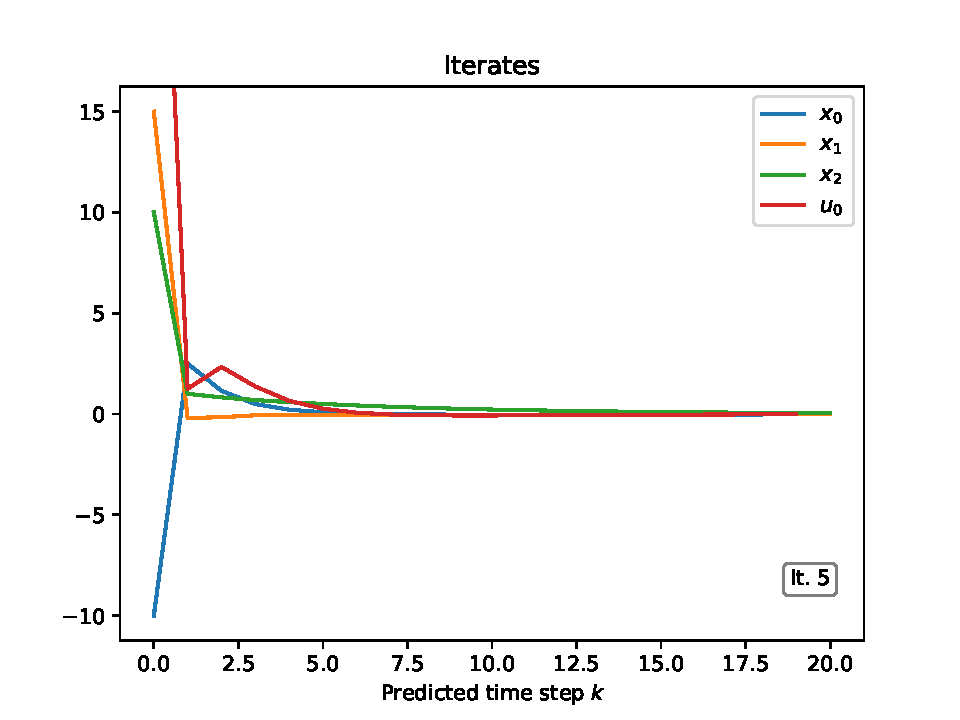
\includegraphics[width=0.7\textwidth]{images/Assignment6-2.pdf}
	\caption{Final solution of the nonlinear test case - Initial guess of all zeros.}
	\label{fig:assignment6_2}
\end{figure}



\begin{assignment} \label{assgn:simulate-init}
   Simulate the system and use this as an initial guess.

   You may find that the solver now fails to converge. 
   Why do you think this happens? 
   
   \textbf{Hint.} Plot the state trajectory you used as an initial guess. 
   Does it look like the solution you just obtained in the previous exercise? 
   Why is this important?
\end{assignment}
\begin{flushleft}
	Starting from an initial guess far from the solution, the Newton-Lagrange method struggles to find a descent direction that satisfies the necessary conditions for optimality.
	Without using line search, the solver diverges in 9 iterations, the evolution of the states can be seen in figure \ref{fig:assignment6_3}.
	The initial guess is crucial for the solver to converge to a meaningful solution.
\end{flushleft}
\begin{lstlisting}[style=python]
	# Output - Last iteration

	it.    8 | JN = 1.04e+06 | ||h||2 = 8.24e+04
	Using Linesearch? False
	Diverged
\end{lstlisting}
\begin{figure}[H]
	\centering
	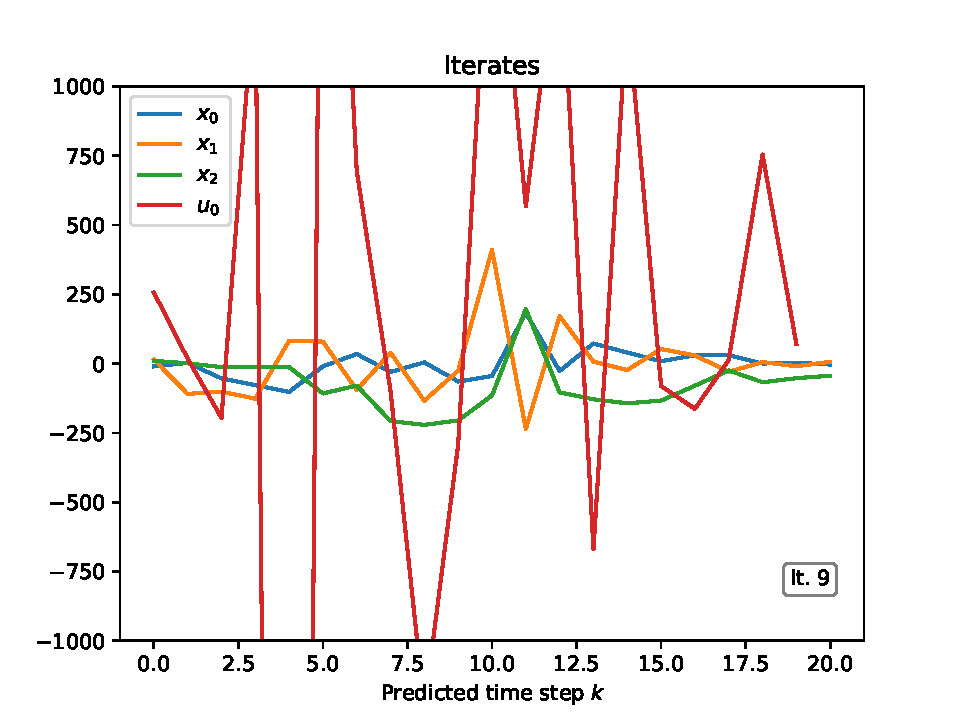
\includegraphics[width=0.7\textwidth]{images/Assignment6-3.pdf}
	\caption{Final solution of the nonlinear test case}
	\label{fig:assignment6_3}
\end{figure}



\subsection{Adding Line Search}

\begin{assignment}
   Implement line search and the experiment of \cref{assgn:simulate-init}. 
   Use 
	\[ 
		\phi(z) = J_N(z) + c \nrm{h(z)}_1 
	\]
	as a merit function (see \texttt{problem.build\_cost\_and\_constraint}). 

	\textbf{Hint.} Make sure to set \texttt{linesearch=True} in the \texttt{cfg} argument of the solver, 
	which is expected to be an instance of \texttt{NewtonLagrangeCfg}.
	
   Now does it converge? Give the output of the method at the final iterate and use this 
   to argue that your method indeed converged to something meaningful. 
   Do you notice any difference with respect to the solution in \cref{assgn:62}? 
   How do you explain this?
\end{assignment}
\begin{flushleft}
	The evolution of the states might differ significantly between cases where the initial approximation is good, Assignment 6.2, versus bad, now.  
	Line search plays a critical role in "guiding" the solver toward the a meaningful solution reducing the step size, added to the log of the solver, significantly to ensure feasibility. Thanks to it, the solver now converges in 79 iterations.
	From the gif can be seen that the states deviate noticeably before settling into a plausible trajectory which resemble the one obtained in Assignment 6.2.
	These unusual behaviors during early iterations are a conseguence of the correction required to compensate for the bad starting point.
\end{flushleft}
\begin{lstlisting}[style=python]
	# Output - Last iteration

	it.   78 | JN = 2.26e+02 | ||h||2 = 8.24e-10 | alpha = 1.00e+00
	Using Linesearch? True
	Converged
\end{lstlisting}
\begin{figure}[H]
	\centering
	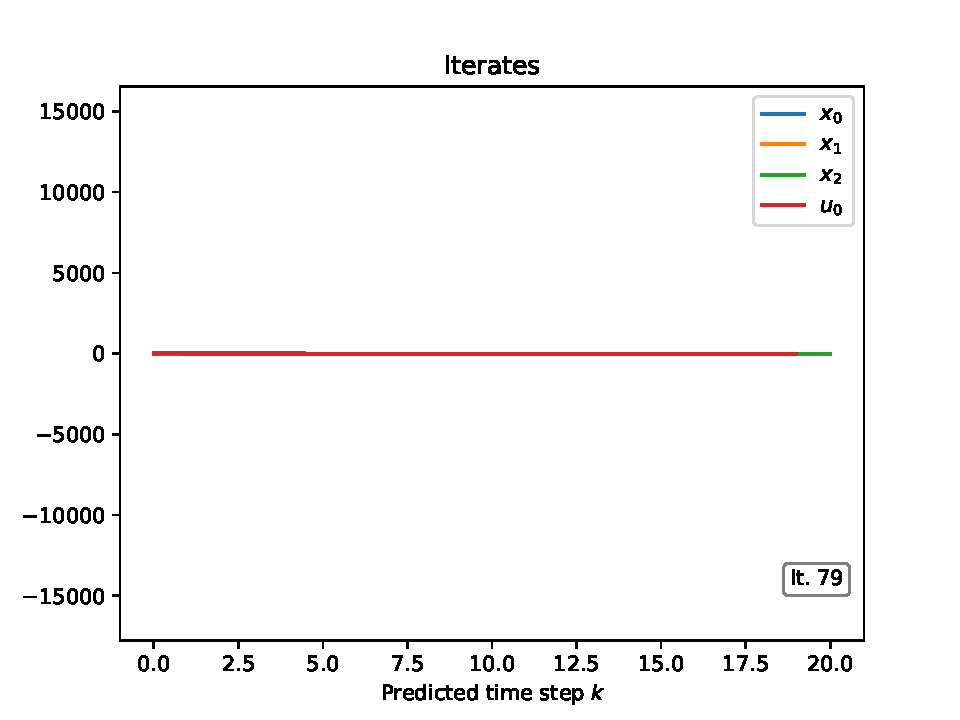
\includegraphics[width=0.7\textwidth]{images/Assignment6-4.pdf}
	\caption{Final solution of the nonlinear test case using linesearch.}
	\label{fig:assignment6_4}
\end{figure}



\begin{assignment}
   Run it on the parking example. Use initial condition all zeros (except $x_0 = $\texttt{problem.x0}).
   
	Does it converge? Why? 
	
	\textbf{Hint. } During the Newton-Lagrange iterations, check whether the Hessian of the QP cost is positive definite.
\end{assignment}
\begin{flushleft}
	The solver does not converge because the Hessian of the cost is not positive definite. 
	This is proven by a check performed in the code which will print in yellow "Warning: Qk is not positive definite!" whenever this happens (frequently).
	Figure \ref{fig:assignment64-parking} shows the trajectory of the car, it is clear that the orgin, parking spot, is not reached.
\end{flushleft}
\begin{figure}[H]
	\centering
	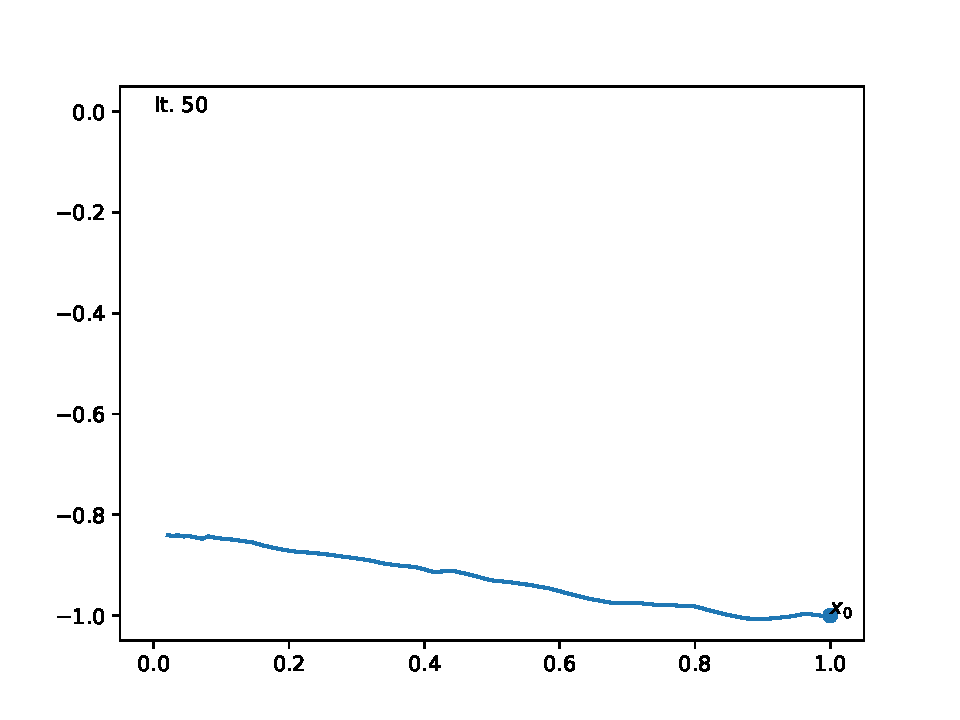
\includegraphics[width=0.7\textwidth]{images/parking_regularize-False-maxiter50.pdf}
	\caption{Final solution of the parking case without using regularization.}
	\label{fig:assignment64-parking}
\end{figure}

\subsection{Adding Regularization}

\begin{assignment}
	Implement regularization in the function \texttt{regularize}. This method should 
	check whether the QP is convex. 
	If not, it should add $\lambda I$ to the Hessian $\overline{Q}$ of the cost function, where $\lambda$ is 
	(approximately) the smallest constant such that $\overline{Q} + \lambda I$ is positive definite.
	To do so set $\lambda = 10^{-6}$ and double it every time the result is not positive definite. 
	
	With this modification, run the method again on the Parking problem. Does it converge? 
	\textbf{Hint.}  Make sure to set \texttt{cfg.regularize} to \texttt{True}!
\end{assignment}
\begin{flushleft}
	Implementing regularization, as shown by the code below, the solver converges in 57 iterations. 
	The trajectory followed by the car to reach the parking spot is shown in \ref{fig:assignment65-parking}.
\end{flushleft}
\begin{lstlisting}[style=python]
	def regularize(qp: problem.NewtonLagrangeQP):
		for _ in range(qp.Qk.shape[0]):
			Q_bar = qp.Qk[_]
			_lambda = 1e-6
			while not is_posdef(Q_bar):
				Q_bar += _lambda * np.eye(Q_bar.shape[0])
				_lambda *= 2
\end{lstlisting}
\begin{figure}[H]
	\centering
	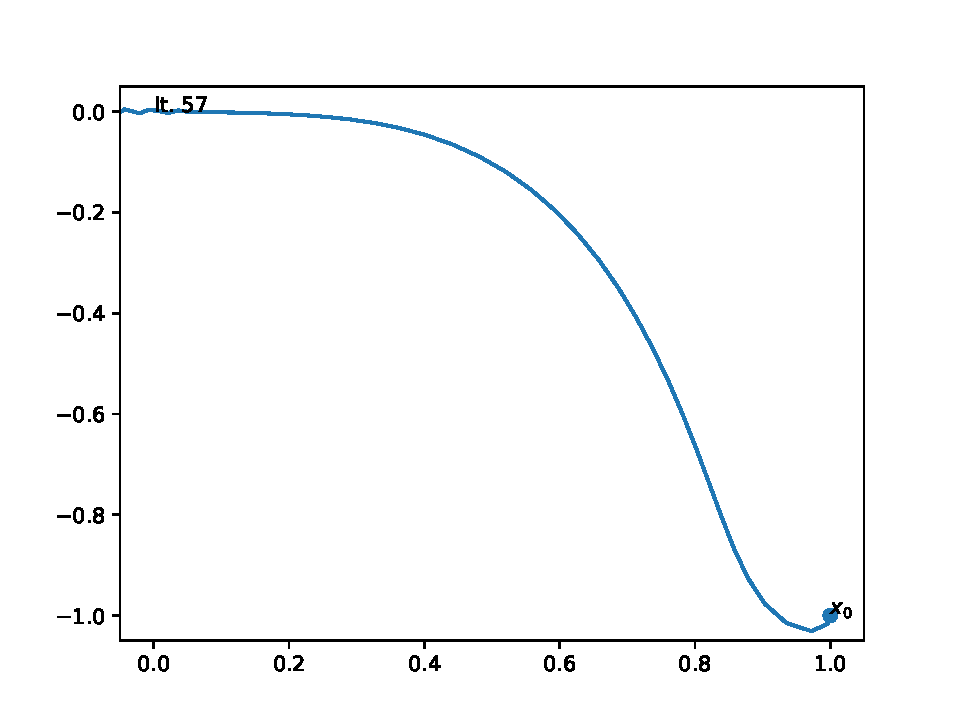
\includegraphics[width=0.7\textwidth]{images/parking_regularize-True-maxiter70.pdf}
	\caption{Final solution of the parking case using regularization.}
	\label{fig:assignment65-parking}
\end{figure}


 


\end{document}